% ------------------------------------------------------------------------
% Nazwa:    Szkielet dokument 'typu praca dyplomowa'
% źródło:   http://www.ee.pw.edu.pl/~szewczyk/
% Data:     7 stycznia 2005
% ------------------------------------------------------------------------

%\documentclass[12pt,notitlepage,oneside]{book}
\documentclass[12pt,oneside]{article}

    % ------------------------------------------------------------------------
% PAKIETY
% ------------------------------------------------------------------------

%różne pakiety matematyczne, warto przejrzeć dokumentację, muszą być powyżej ustawień językowych.
\usepackage{mathrsfs}   %Różne symbole matematyczne opisane w katalogu ~\doc\latex\comprehensive. Zamienia \mathcal{L} ze zwykłego L na L-transformatę.
\usepackage{eucal}      %Różne symbole matematyczne.
\usepackage{amssymb}    %Różne symbole matematyczne.
\usepackage{amsmath}    %Dodatkowe funkcje matematyczne, np. polecenie \dfac{}{} składające ułamek w trybie wystawionym (porównaj $\dfrac{1}{2}$, a $\frac{1}{2}$).

%język polski i klawiatura
\usepackage[polish]{babel}
\usepackage[OT4]{polski}
\usepackage[library/utf8]{inputenc}                       %Strona kodowa polskich znaków.

%obsługa pdf'a
\usepackage[pdftex,usenames,dvipsnames]{color}      %Obsługa kolorów. Opcje usenames i dvipsnames wprowadzają dodatkowe nazwy kolorów.
\usepackage[pdftex,pagebackref=false,draft=false,pdfpagelabels=false,colorlinks=true,urlcolor=black,linkcolor=black,citecolor=black,pdfstartview=FitH,pdfstartpage=1,pdfpagemode=UseOutlines,bookmarks=true,bookmarksopen=true,bookmarksopenlevel=2,bookmarksnumbered=true,pdfauthor={Tomasz
Flis,Dominik Kornaus},pdftitle={dokument},pdfsubject={Praca
magisterska},pdfkeywords={},unicode=true]{hyperref}
%Opcja pagebackref=true dotyczy bibliografii: pokazuje w spisie literatury
%numery stron, na których odwołano się do danej pozycji.

%bibliografia
\usepackage[numbers,sort&compress]{natbib}  %Porządkuje zawartość odnośników do literatury, np. [2-4,6]. Musi być pod pdf'em, a styl bibliogfafii musi mieć nazwę z dodatkiem 'nat', np. \bibliographystyle{unsrtnat} (w kolejności cytowania).
\usepackage{library/hypernat}                       %Potrzebna pakietowi natbib do wspołpracy z pakietem hyperref (ważna kolejność: 1. hyperref, 2. natbib, 3. hypernat).

%grafika i geometria strony
\usepackage{extsizes}           %Dostępne inne rozmiary czcionek, np. 14 w poleceniu: \documentclass[14pt]{article}.
\usepackage[final]{graphicx}
\usepackage[a4paper,left=3.5cm,right=2.5cm,top=2.5cm,bottom=2.5cm]{geometry}

%strona tytu�owa
\usepackage{titlepage}

%inne
\usepackage[hide]{library/todo}                     %Wprowadza polecenie \todo{treść}. Opcje pakietu: hide/show. Polecenie \todos ma być na końcu dokumentu, wszystkie \todo{} po \todos sa ignorowane.
%\usepackage[basic,physics]{circ}            %Wprowadza środowisko circuit do rysowania obwodów elektrycznych. Musi być poniżej pakietow językowych.
\usepackage[sf,bf,outermarks]{titlesec/titlesec}     %Troszczy się o wygląd tytułów rozdziałów (section, subsection, ...). sf oznacza czcionkę sans serif (typu arial), bf -- bold. U mnie: oddzielna linia dla nagłówku paragraph. Patrz tez: tocloft -- lepiej robi format spisu treści. \usepackage{tocloft}                        %Troszczy się o format spisu trsci. \usepackage{library/expdlist}    %Zmienia definicję środowiska description, daje większe możliwości wpływu na wygląd listy.
\usepackage{flafter}     %Wprowadza parametr [tb] do polecenia \suppressfloats[t] (polecenie to powoduje nie umieszczanie rysunków, tabel itp. na stronach, na których jest to polecenie (np. może być to strona z tytułem rozdziału, który chcemy żeby był u samej góry, a nie np. pod rysunkiem)).
\usepackage{array}       %Ładniej drukuje tabelki (np. daje wiecej miejsca w komorkach -- nie są tak ścieśnione, jak bez tego pakietu).
\usepackage{listings}    %Listingi programow.
\lstset{language=C++,basicstyle=\scriptsize}
\usepackage[format=hang,labelsep=period,font={bf,footnotesize}]{caption} %Formatuje podpisy pod rysunkami i tabelami. Parametr 'hang' powoduje wcięcie kolejnych linii podpisu na szerokosc nazwy podpisu, np. 'Rysunek 1.'. \usepackage{appendix}    %Troszczy się o załączniki. \usepackage{floatflt}    %Troszczy się o oblewanie rysunkow tekstem.
\usepackage{appendix}    %Troszczy się o załączniki.
\usepackage{floatflt}    %Troszczy się o oblewanie rysunkow tekstem.
\usepackage{here}        %Wprowadza dodtkowy parametr umiejscowienia rysunków, tabel, itp.: H (duże). Umiejscawia obiekty ruchome dokladnie tam gdzie są w kodzie źródłowym dokumentu.
\usepackage{makeidx}     %Troszczy się o indeks (skorowidz).
\usepackage{fnpos}		%Umieszcza przypisy tam gdzie trzeba
%\makeFNbottom
\usepackage{inputenc}
%nieużywane, ale potencjalnie przydatne
\usepackage{sectsty}           %Formatuje nagłówki, np. żeby były kolorowe -- polecenie: \allsectionsfont{\color{Blue}}.
\usepackage{tocloft}
\usepackage{expdlist}
%\usepackage{version}           %Wersje dokumentu.
%\usepackage{fancyhdr}          %Dodaje naglowki jakie się chce.
%\usepackage{antyktor}          %Składa dokument przy użyciu Antykwy Toruńskiej.
%\usepackage{antpolt}           %Składa dokument przy użyciu Antykwy Ptawskiego.
%\usepackage[left]{showlabels}  %Pokazuje etykiety, ale kiepsko bo nie mieszczą się na marginesie (można od biedy powiększyć margines w pakiecie geometry powyżej). Nie może być na górze (pakiet).
\usepackage{fancyhdr}		%Pagina
\usepackage{subfig}
\usepackage{indentfirst}
\usepackage{fmtcount}
\usepackage[table]{xcolor}
\usepackage{setspace}
    % ------------------------------------------------------------------------
% USTAWIENIA
% ------------------------------------------------------------------------

% ------------------------------------------------------------------------
%   Kropki po numerach sekcji, podsekcji, itd.
%   Np. 1.2. Tytuł podrozdziału
% ------------------------------------------------------------------------
\makeatletter
    \def\numberline#1{\hb@xt@\@tempdima{#1.\hfil}}                      %kropki w spisie treści
    \renewcommand*\@seccntformat[1]{\csname the#1\endcsname.\enspace}   %kropki w treści dokumentu
\makeatother

% ------------------------------------------------------------------------
%   Numeracja równań, rysunków i tabel
%   Np.: (1.2), gdzie:
%   1 - numer sekcji, 2 - numer równania, rysunku, tabeli
%   Uwaga ogólna: o otoczeniu figure ma być najpierw \caption{}, potem \label{}, inaczej odnośnik nie działa!
% ------------------------------------------------------------------------
\makeatletter
    \@addtoreset{equation}{section} %resetuje licznik po rozpoczęciu nowej sekcji
    \renewcommand{\theequation}{{\thesection}.\@arabic\c@equation} %dodaje kropkę

    \@addtoreset{figure}{section}
    \renewcommand{\thefigure}{{\thesection}.\@arabic\c@figure}

    \@addtoreset{table}{section}
    \renewcommand{\thetable}{{\thesection}.\@arabic\c@table}
\makeatother

% ------------------------------------------------------------------------
% Tablica
% ------------------------------------------------------------------------
\newenvironment{tablica}[3]
{
    \begin{table}[!tb]
    \centering
    \caption[#1]{#2}
    \vskip 9pt
    #3
}{
    \end{table}
}

% ------------------------------------------------------------------------
% Dostosowanie wyglądu pozycji listy \todos, np. zamiast 'p.' jest 'str.'
% ------------------------------------------------------------------------
\renewcommand{\todoitem}[2]{%
    \item \label{todo:\thetodo}%
    \ifx#1\todomark%
        \else\textbf{#1 }%
    \fi%
    (str.~\pageref{todopage:\thetodo})\ #2}
\renewcommand{\todoname}{Do zrobienia...}
\renewcommand{\todomark}{~uzupełnię}

% ------------------------------------------------------------------------
% Definicje
% ------------------------------------------------------------------------
\def\nonumsection#1{%
    \section*{#1}%
    \addcontentsline{toc}{section}{#1}%
    }
\def\nonumsubsection#1{%
    \subsection*{#1}%
    \addcontentsline{toc}{subsection}{#1}%
    }
\reversemarginpar %umieszcza notki po lewej stronie, czyli tam gdzie jest więcej miejsca
\def\notka#1{%
    \marginpar{\footnotesize{#1}}%
    }
\def\mathcal#1{%
    \mathscr{#1}%
    }
\newcommand{\atp}{ATP/EMTP} % Inaczej: \def\atp{ATP/EMTP}

% ------------------------------------------------------------------------
% Inne
% ------------------------------------------------------------------------
\frenchspacing                      %nie pamiętam co to jest, ale używam
%\flushbottom                       %nie pamiętam co to jest, ale nie używam
%\raggedbottom                      %nie pamiętam co to jest, ale nie używam
\interfootnotelinepenalty=10000		%nie dziel footnote na kilka stron
\hyphenation{ATP/-EMTP}             %dzielenie wyrazu w żądanym miejscu
\setlength{\parskip}{3pt}           %odstęp pomiędzy akapitami
\linespread{1.3}                    %odstęp pomiędzy liniami (interlinia)
\setcounter{tocdepth}{4}            %uwzględnianie w spisie treęci czterech poziomów sekcji
\setcounter{secnumdepth}{4}         %numerowanie do czwartego poziomu sekcji włącznie
%wygląd nagłówków
\titleformat\paragraph[hang]{\normalfont\sffamily\bfseries}{\theparagraph}{1em}{}
%\definecolor{niebieski}{rgb}{0.0,0.0,0.5}

%\pagestyle{fancy}
%% zmiana liter w zywej paginie na male
%%\renewcommand{\chaptermark}[1]{\markboth{#1}{}}
%\renewcommand{\sectionmark}[1]{\markboth{ #1}{}}
%\renewcommand{\subsectionmark}[1]{\markboth{ #1}{}}
%\renewcommand{\sectionmark}[1]{\markright{ #1}}
%%\renewcommand{\subsectionmark}[1]{\markleft{\thesubsection\ #1}}
%%\renewcommand{\subsectionmark}{} % zakomentarzuj jesli maja byc rowniez podrozdzialy
%\fancyhf{} % usun bierzace ustawienia pagin
%\fancyhead[LE,RO]{\small\bfseries\thepage}
%\fancyhead[LO]{\small\bfseries\rightmark}
%\fancyhead[RE]{\small\bfseries\leftmark}
%\renewcommand{\headrulewidth}{0.5pt}
%\renewcommand{\footrulewidth}{0pt}
%\addtolength{\headheight}{0.5pt} % pionowy odstep na kreske
%\fancypagestyle{plain}
%{%
%	\fancyhead{} % usun p. gorne na stronach pozbawionych numeracji (plain)
%	\renewcommand{\headrulewidth}{0pt} % pozioma kreska
%}
\pagestyle{fancy}
\renewcommand{\sectionmark}[1]{\markboth{#1}{}}
\renewcommand{\subsectionmark}[1]{\markright{\thesubsection\ #1}}
\fancyhf{}
\fancyhead[LE,RO]{\small\bfseries\thepage}
\fancyhead[LO]{\small\bfseries\rightmark}
\fancyhead[RE]{\small\bfseries\leftmark}
\renewcommand{\headrulewidth}{0.5pt}
\renewcommand{\footrulewidth}{0pt}
\addtolength{\headheight}{0.5pt}
\fancypagestyle{plain}
{%
 \fancyhead{}
 \renewcommand{\headrulewidth}{0pt}
}

\definecolor{code_back}{rgb}{0.9,0.9,0.9}

    \title{INTELIGENTNY SYNTETYZATOR TWARZY LUDZKIEJ NA PODSTAWIE SZKICÓW
    PROFILI}
    \author{Tomasz Flis\\Dominik Kornaus}

    %polecenia zdefiniowane w pakiecie strona_tytulowa.sty
    \academy{Akademia Gorniczo-Hutnicza w~Krakowie}
    \institute{Wydzial Elektrotechniki, Automatyki, Informatyki i Elektroniki}
    \specialization{INFORMATYKA}
    \speciality{Systemy komputerowe}
    \promoter{dr inż. T. Szuba; prof. nzw. AGH}
    \project{PRACA MAGISTERSKA}
    \city{Krakow}
    \year{2011}
    %\draft  %odkomentarzuj tę linię, jeśli wydruk ma być draftem -- wprowadza informację o drafcie na stronie tytułowej
    %koniec poleceń zdefiniowanych przez pakiet strona_tytulowa.sty

    %skorowidz - nie używam
    %\makeindex
    %koniec skorowidza

\begin{document}
    \renewcommand{\figurename}{\bf Ilustracja}    %musi byc pod \begin{document}, bo w~tym miejscu pakiet 'babel' narzuca swoje ustawienia
    \renewcommand{\tablename}{Tab.}     %j.w.
    %jeśli numerki rzymskie to roman
    \pagenumbering{arabic}               %numeracja stron: rzymska
    \pagestyle{fancy}
    \thispagestyle{empty}               %na tej stronie: brak numeru
    \titlepage                     %strona tytułowa tworzona przez pakiet strona_tytulowa.tex

    %podziękowania
    \newpage
    ~   %potrzebne dla \vfill
    \vfill
    {\sffamily
    \begin{flushright}
        \begin{tabular}[c]{p{9cm}}
        \centering
        \noindent
         Pragniemy złożyć najserdeczniejsze podziękowania dla:
         
         Pana dr inż. Marka Gajęckiego, Kierownika Katedry Informatyki, za
         możliwość realizacji niniejszej pracy
         
         oraz
         
%         Składamy serdeczne podziękowania 
         Pana dr inż. Tadeusza Szuby za niezwykłą
         cierpliwość, cenne uwagi i wskazówki udzielone
         nam w trakcie pisania tej pracy magisterskiej.
        \end{tabular}
    \end{flushright}
    }
    \vskip0.5in
    \thispagestyle{empty}
    \newpage
    %koniec podziękowań

    \thispagestyle{empty}
    %formatowanie spisu treści i~nagłówków
    %jeśli chcemy numerki rzymski to roman
    \renewcommand{\thepage}{\arabic{page}}
    \renewcommand{\cftbeforesecskip}{8pt}
    \renewcommand{\cftsecafterpnum}{\vskip 8pt}
    \renewcommand{\cftparskip}{3pt}
    \renewcommand{\cfttoctitlefont}{\Large\bfseries\sffamily}
    \renewcommand{\cftsecfont}{\bfseries\sffamily}
    \renewcommand{\cftsubsecfont}{\sffamily}
    \renewcommand{\cftsubsubsecfont}{\sffamily}
    \renewcommand{\cftparafont}{\sffamily}
    %koniec formatowania spisu treści i nagłówków
	\hypersetup{linkcolor=black}
    \begin{spacing}{0.8}
    \tableofcontents    %spis treści
    \end{spacing}
    \newpage

	\thispagestyle{empty}
    \nonumsection{Wykaz ważniejszych skrótów i~oznaczeń}
\suppressfloats[t]

\begin{description}[\setleftmargin{65pt}\setlabelstyle{\bfseries}]
    \leftskip=1cm
    \item[derywacja]	w językoznawstwie to proces słowotwórczy polegający na
    tworzeniu wyrazów pochodnych poprzez dodawanie do podstawy słowotwórczej
    sufiksów i prefiksów
    \item[fraktal]		w znaczeniu potocznym oznacza zwykle obiekt samo-podobny
    (tzn. taki, którego części są podobne do całości) albo nieskończenie
    subtelny (ukazujący subtelne detale nawet w wielokrotnym powiększeniu)
    \item[CSG]			(ang. Constructive Solid Geometry) w grafice komputerowej i
    zastosowaniach CAD technika definiowania nowych brył poprzez łączenie innych brył
    regularyzowanymi działaniami boolowskimi: sumą, częścią wspólną i różnicą. Regularyzowane
    operatory tym różnią się od zwykłych działań na zbiorach punktów, że gwarantują,
    iż wynikiem działania będzie nadal bryła, a więc obiekt posiadający objętość. Wynikiem
    regularyzowanej operacji nie będzie zatem nigdy punkt, odcinek lub płaszczyzna.
    \item[ray-tracing]	śledzenie promieni --- technika
    generowania fotorealistycznych obrazów scen trójwymiarowych. Opiera się na analizowaniu tylko
    tych promieni światła, które trafiają bezpośrednio do obserwatora. W rekursywnym
    śledzeniu promieni bada się dodatkowo promienie odbite zwierciadlane oraz załamane.
    Ponadto umożliwia łatwą realizację CSG, a także wizualizację idealnych,
    opisywanych formułami matematycznymi obiektów.
%    \item[PE]			Portable Executable
%    \item[$f$]        częstotliwość źródeł sieci elektroenergetycznej
%    \item[$\omega$]   pulsacja źródeł sieci elektroenergetycznej
%    \item[$\omega_0$] pulsacja drgań własnych obwodu drgającego
%    \item[$U_n$]      napięcie znamionowe sieci elektroenergetycznej, wartość skuteczna napięcia międzyfazowego sieci
%    \item[$E$]        wartość skuteczna fazowego napięcia znamionowego sieci
\end{description}

    \newpage

    %spis rysunków i~tablic
    %format spisu treści dotyczy tylko tych spisów, które są poniżej
%    \renewcommand{\cftparskip}{3pt}
%    \clearpage
%    \renewcommand{\cftloftitlefont}{\Large\bfseries\sffamily}
%    \listoffigures
%    \addcontentsline{toc}{section}{Spis rysunków}
%    \newpage
%    \renewcommand{\cftlottitlefont}{\Large\bfseries\sffamily}
%    \listoftables
%    \addcontentsline{toc}{section}{Spis tablic}
%    \newpage
    %powrót do czerwonego koloru dla dalszych odnośników (spis literatury, przy włączonym pokazywaniu numerów stron, do których odnoszą się poszczególne pozycje)
%    \hypersetup{linkcolor=red}
    %koniec spisu rysunków i~tablic

    %przeniesienie wartości licznika stron na strony numerowane innym stylem (arabic)
    \newcounter{licznikStron}
    \setcounter{licznikStron}{\value{page}}
    \pagenumbering{arabic}
    \setcounter{page}{\value{licznikStron}}
    %koniec przeniesienia...

    %treść główna dokumentu
    %\section*{Abstract}
%\thispagestyle{empty}
%Grafika trójwymiarowa to jedna z najdynamiczniej rozwijających się dziedzin
%informatyki. Nieustanne dążenie do uzyskania fotorealistycznego obrazu
%wymusza dopracowywanie elementów budujących wirtualny świat oraz technik i
%programów pozwalających na uzyskanie jak najlepszych efektów w jak najkrótszym
%czasie.
%
%W tej pracy prezentujemy technikę, która pozwala na znaczne przyspieszenie
%procesu tworzenia trójwymiarowego modelu głowy dzięki wykorzystaniu wymyślonych
%przez nas metod generowania modelu ze szkiców profili głowy. Użycie
%prezentowanych metod pozwala na zautomatyzowanie części procesu odtwarzania
%obiektu i daje w efekcie podstawowe odwzorowanie analizowanego obiektu.
%Przedstawiona technika jako dane wejściowe wykorzystuje obrazy dwuwymiarowe
%zawierające rzuty głowy oraz informację o rozmieszczeniu na nich punktów
%charakterystycznych. Algorytm pozwala na uzyskanie przybliżonej reprezentacji
%trójwymiarowej głowy przy małej ilości danych, zwiększając swą dokładność wraz
%ze wzrostem danych z różnych rzutów.
%
%\newpage
\section*{Abstract}
Three-dimensional graphics is one of the fastest growing disciplines of
computer science. The pursuite of photorealistic images is a constant
process that forces developement of new algorithms and software to obtain the
best results in the shortest possible time.

In this paper we present the technique aimed to drastically decrease the time
needed to create 3D models of human head using photos of real head. Techniques
described in this paper allows creation of models to be automated and
requires only small amount of data to give rough model of analysed head.
    \newpage
    \section{Wstęp}
Grafika komputerowa i gry komputerowe napędzają rozwój sprzętu
komputerowego. Jeszcze nie tak dawno gry 2D były hitem, dzisiaj każda szanująca
się gra jest osadzona w świecie 3D z niezwykle realistyczną grafiką. Świat we
współczesnych grach jest tak realistyczny, że czasami trudno jest już go
odróżnić od świata rzeczywistego. Zaawansowane technologie związane z grafiką
trójwymiarową są również wykorzystywane w innych dziedzinach np. kinematografii,
komputerowo wspomaganym projektowaniu, medycynie i wielu innych.

{
\addtocounter{footnote}{1}
\begin{figure}[h!]
  \centering
  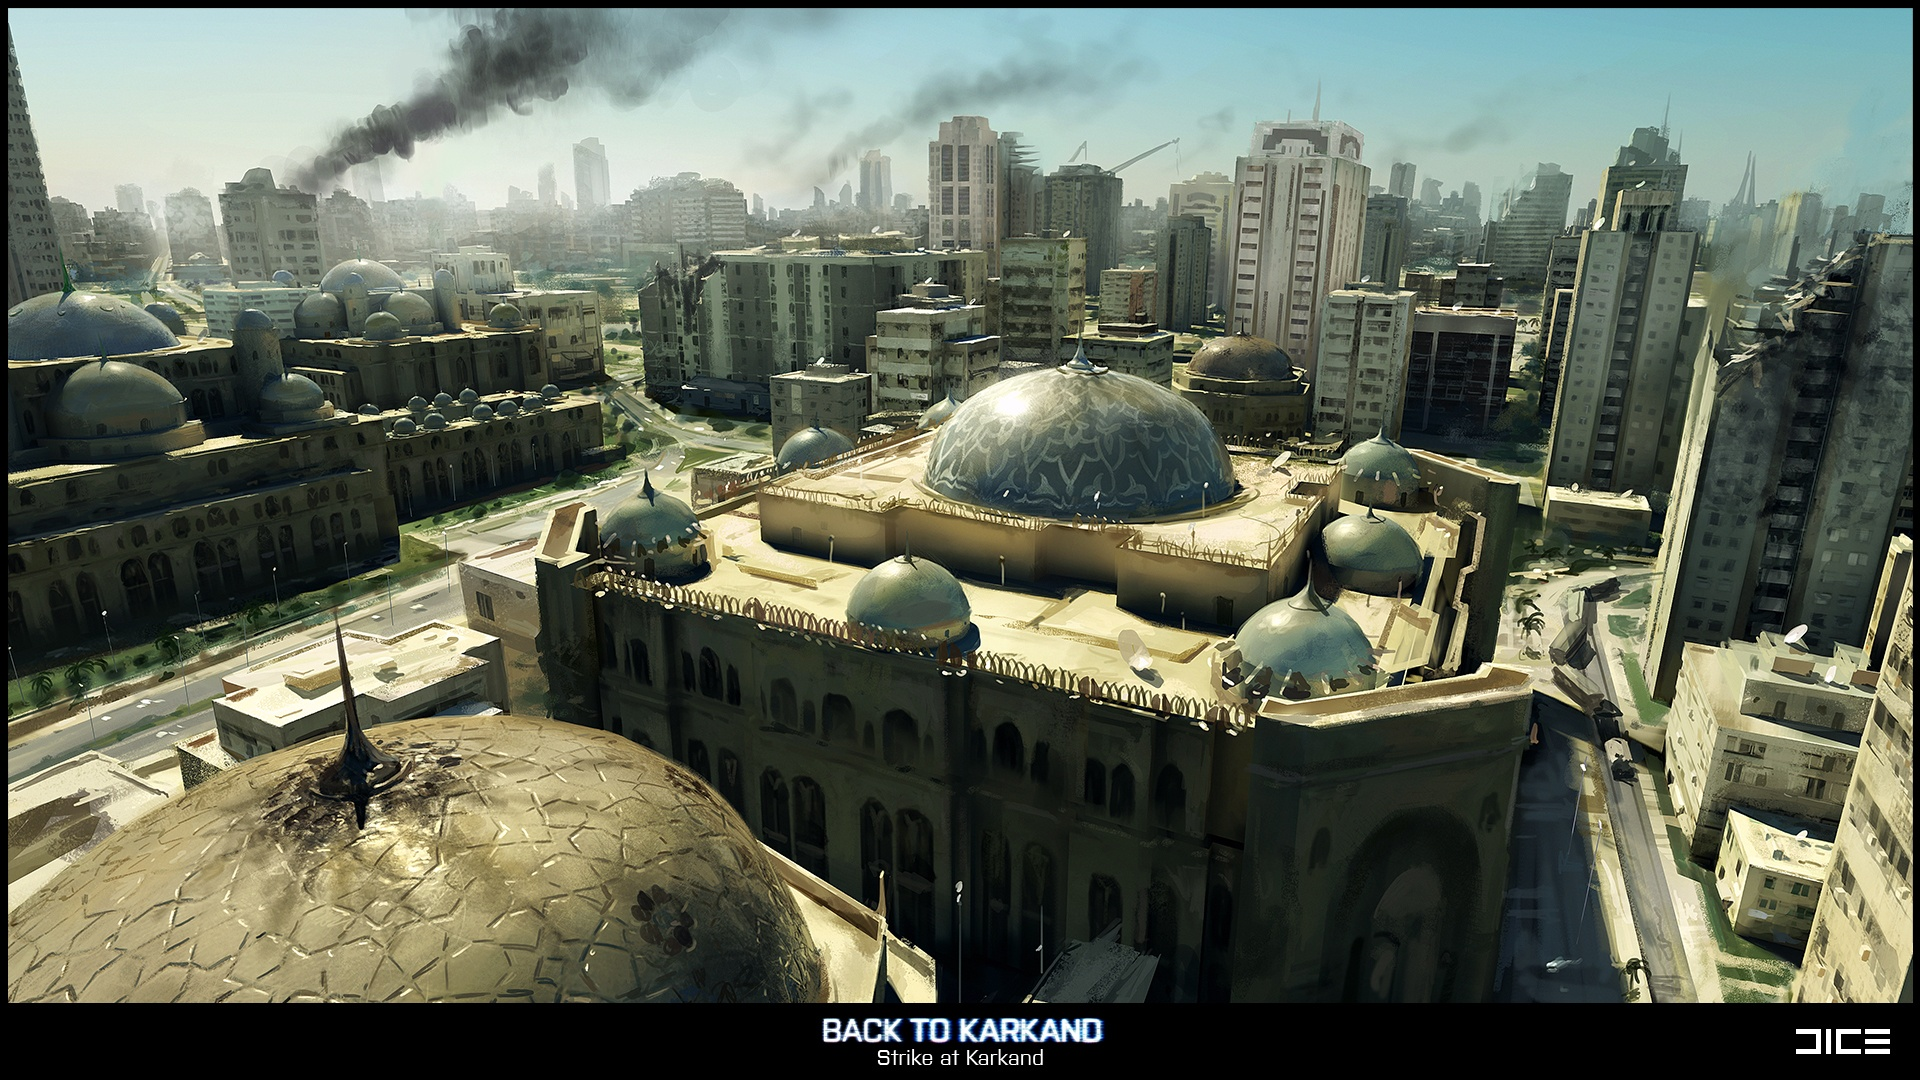
\includegraphics[width=0.8\textwidth]{images/bf3_1.jpg}
  \caption[Gra Battlefield 3]{Gra Battlefield 3~$^{\decimal{footnote}}$.}
\end{figure}
\begin{figure}[h!]
  \centering
  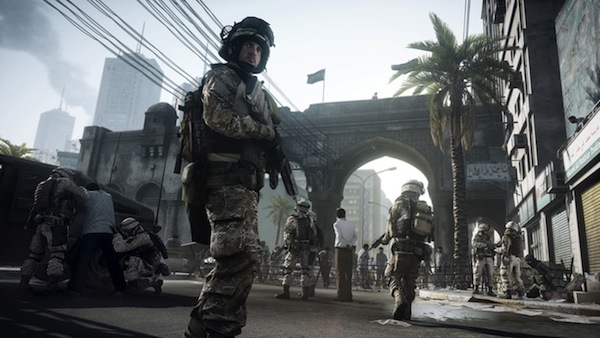
\includegraphics[width=0.8\textwidth]{images/bf3_2.jpg}
  \caption[Gra Battlefield 3 cd.]{Gra Battlefield 3~$^{\decimal{footnote}}$ cd.}
\end{figure}
\footnotetext[\value{footnote}]{\url{http://www.pcgamer.com/2011/05/11/battlefield-3-back-to-karkand-map-pack-detailed/}
%\url{http://www.g4tv.com/thefeed/blog/post/712382/battlefield-3-to-be-the-biggest-launch-in-eas-history/}
}
\addtocounter{footnote}{1}
\begin{figure}[h!]
  \centering
  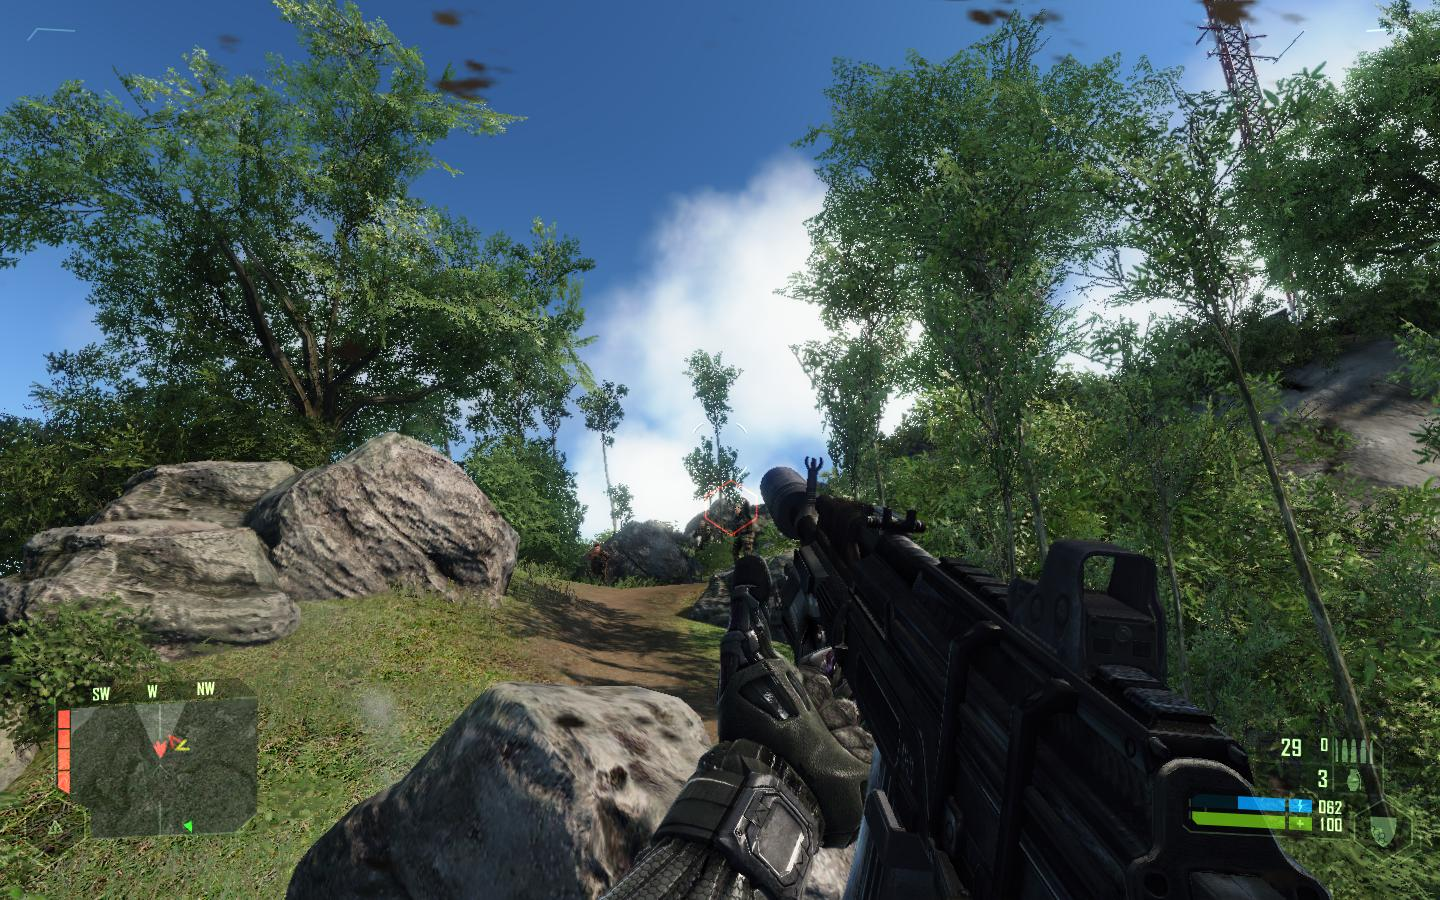
\includegraphics[width=0.8\textwidth]{images/Crysis2.JPG}
  \caption[Gra Crysis 2]{Gra Crysis 2~$^{\decimal{footnote}}$.}
\end{figure}
\footnotetext[\value{footnote}]{\url{http://mattplays.com/game/crysis/}}
}

Głównym problemem w dzisiejszych czasach nie jest stworzenie realistycznego
świata, a realistycznego człowieka. Jednym z ciekawszych projektów poruszających
ten temat jest program o nazwie Emily~\cite{link01}, gdzie rozpoznanie czy jest
to animacja 3D czy prawdziwy człowiek jest praktycznie niemożliwe.

Zastosowanie syntetycznego generowania obiektów 3D ma zastosowanie nie tylko w
grach komputerowych czy w kinematografii, ale również może zostać wykorzystane w
kompresji obrazu. Doszliśmy już do granicy możliwości kompresji obrazu z
wykorzystaniem transformacji
Fouriera~\footnote{\url{http://mathworld.wolfram.com/FourierTransform.html}}
czy transformacji
falkowej~\footnote{\url{http://mathworld.wolfram.com/WaveletTransform.html}}.
Dalszy rozwój w tym kierunku nie daje już dużego skoku na rozmiarze czy jakości
kompresowanego obrazu. Ograniczenie to wymusza nowe podejście do kompresji
obrazu polegające na syntezie obrazu do znanych wzorów, tak jak to robi nasz
mózg --- gdy oglądamy filmy nie musimy widzieć dokładnie jak układają się źdźbła
trawy --- informacja, że na scenie znajduje się trawa wystarczy, tak samo nie
interesuje nas ile jest chmur na niebie --- tylko to, że jest
zachmurzenie. Tak samo można skompresować obraz przedstawiający ludzką twarz ---
nie interesuje nas faktura skóry twarzy czy rozmieszczenie włosów na głowie
aktora, nawet niekiedy nie interesuje nas sam wygląd aktora jeśli go nie znamy,
interesuje nas zaś, w której scenie dany aktor występuje i co takiego robi/mówi.
Gdybyśmy więc kompresując film zapisywali ogólny wygląd aktora w postaci
parametrów modelu człowieka i w kolejnych klatkach animacji zmieniali tylko
parametry opisujące mimikę twarzy aktora mielibyśmy doskonałą kompresję --- a
jakość filmu zależałaby tylko od szczegółowości modelu obiektów.

Niniejsza praca skupia się głównie na twarzy ludzkiej, opisuje powierzchownie
jej budowę (kształt) oraz proponuje formę opisu twarzy (wiedza) w oparciu o
gramatykę kształtu.

W internecie jest dość niewiele aplikacji generujących twarz trójwymiarową na
podstawie zdjęć. Jedną z tych, które udało nam się znaleźć jest FaceGen firmy
Singular~\cite{link04}. Aplikacja ta jest bardziej nastawiona na edycje twarzy
(ruchy ust, ruchy powiek, mimika), generowanie twarzy na podstawie profili
jest tylko dodatkiem. Aplikacja potrafi nawet na podstawie zdjęć przygotować
odpowiednią teksturę, która po nałożeniu na model polepsza realizm twarzy.

Synteza twarzy ludzkiej jest młodą dziedziną, gdyż dopiero od niedawna sprzęt
komputerowy jest na tyle wydajny, by w rozsądnym czasie wygenerować obiekt.
Dość trudną sprawą w całym zadaniu jest analiza obrazu, rozpoznanie gdzie na
obrazie znajdują się punkty charakterystyczne twarzy takie jak oczy, usta czy
nos. Niniejsza praca nie będzie wgłębiała się w elementy lokalizowania
twarzy na zdjęciu czy wyszukiwaniu punktów charakterystycznych, na ten
temat jest mnóstwo materiałów w sieci (od metod gradientowych po analizę
koloru). Skupimy się głównie na ręcznym wyznaczeniu charakterystycznych
elementów twarzy, których wierne przeniesienie na model komputerowy będzie
kluczowe w celu wygenerowania twarzy trójwymiarowej. Drugim istotnym
zagadnieniem poruszonym w tej pracy jest przetransformowanie wiedzy uzyskanej w
poprzednim etapie na gramatykę kształtu twarzy. Po uzyskaniu punktów
charakterystycznych i mając opis twarzy za pomocą gramatyki kształtu bądź jej
prototyp, wygenerowanie obiektu nie powinno być kłopotliwe, oczywiście jeśli tą
wiedzę posiadamy. Zadanie to nie jest proste ze względu na skomplikowany
wygląd twarzy ludzkiej, praktycznie niewielka zmiana położenia oczu, nosa bądź
ust, całkowicie może zmienić wygląd twarzy.

\subsection{Cel i~zakres pracy}
Celem pracy jest opisanie skomplikowanej budowy twarzy ludzkiej i zaproponowanie
modelu jej opisu w postaci gramatyki kształtu, który wraz z informacją o
położeniu punktów charakterystycznych na obrazie wygeneruje obiekt 3D w pewnym
zakresie zbliżony do twarzy źródłowej. Będziemy się starać, aby model ten był na
tyle uniwersalny, by niewielkim nakładem pracy móc opisać nie tylko
twarz ale całe ciało ludzkie. Praktyczną częścią pracy będzie stworzenie
niewielkiej aplikacji wykorzystującej wyżej wspomniany model, która na
podstawie szkiców bądź zdjęć profili twarzy ludzkiej będzie generowała model 3D
twarzy. Przy odpowiednim zdefiniowaniu i sparametryzowaniu schematu zestaw
danych mógłby jednoznacznie identyfikować osobę. Mogłoby to być wykorzystywane w
rozpoznawaniu osób na podstawie profili. Rozszerzenie pracy o wyciąganie danych
z dowolnych zdjęć ułatwiłoby wyszukiwanie i identyfikację osoby w tłumie, na
podstawie szczątkowych danych z obrazu (twarz częściowo zasłonięta, lekko
obrócona).

\subsection{Streszczenie pracy}
Całość pracy jest podzielona na siedem rozdziałów, w których zawarto
odpowiednio:
\begin{itemize}
  \item rozdział 1 zawiera opis zagadnienia poruszanego w pracy;
  \item rozdział 2 zawiera opis metod przenoszenia obiektów do 3D;
  \item rozdział 3 zawiera wstęp teoretyczny do gramatyk kształtów;
  \item rozdział 4 zawiera opis spojrzenie na to jak ten problem rozwiązali
  inni;
  \item rozdział 5 zawiera opis koncepcji systemu, co~należy wykonać
  w~praktycznej części pracy;
  \item w rozdziale 6 znajduje się opis implementacji praktycznej części pracy;
  \item w rozdziale 7 znajdują się przykładowe symulacje, eksperymenty z
  aplikacją i ich wyniki;
  \item rozdział 8 zawiera podsumowanie pracy, co udało się wykonać, opis
  napotkanych trudności, jak można rozszerzyć dziedzinę projektu oraz uwagi
  końcowe.
\end{itemize}

    \newpage
    \section{Metody przenoszenia obiektów do 3D}
Odkąd zaczęto wykorzystywać komputerową grafikę trójwymiarową do tworzenia
wirtualnych rzeczywistości zaszła potrzeba wynalezienia sposobu tworzenia jak
najprostszego i zarazem najlepszego sposobu odwzorowywania istniejących
przedmiotów w świecie wirtualnym. Ten rozdział przedstawia opis metodologii oraz
ogólny zarys wykorzystywanych aktualnie algorytmów służących do spełnienia
przedstawionego wymagania.

\subsection{Modelowanie obiektów}
Modelowanie obiektów jest jednym ze sposobów, które wymagają najwięcej
kreatywnej pracy. Modelowanie można zdefiniować jako proces tworzenia
trójwymiarowych obiektów przy użyciu specjalistycznego oprogramowania.
Trójwymiarowy obiekt jest zdefiniowany przy użyciu obiektów matematycznych
takich jak punkt, trójkąty, krzywe, powierzchnie. Na rynku istnieje wiele programów,
których funkcjonalność jest wystarczająca do przygotowania pełnego,
realistycznego modelu. Do najbardziej popularnych można zaliczyć Autodesk
Maya~\footnote{\url{http://usa.autodesk.com/maya/}}, Autodesk 3ds
Max~\footnote{\url{http://usa.autodesk.com/3ds-max/}}, MAXON Cinema
4D~\footnote{\url{http://www.maxon.net/}}, NewTek Lightwave
3D~\footnote{\url{http://www.newtek.com/lightwave.html}}, Pixologic
ZBrush~\footnote{\url{http://www.pixologic.com/zbrush/}}, Luxology
Modo~\footnote{\url{http://www.luxology.com/modo/index.aspx}} bądź darmowy
Blender~\footnote{\url{http://www.blender.org/}}.

Co prawda nie ma ściśle określonych reguł co do etapów występujących w procesie
tworzenia modelu ale ogólnie można wyróżnić kilka logicznych etapów (na
przykładzie modelowania głowy):
\begin{enumerate}
  \item przygotowanie kilku obrazów odniesienia modelowanej głowy;
  \item wstępne wydzielenie linii charakterystycznych;
  \item wykorzystanie krzywych (lub wielokątów) do zamodelowania kształtu głowy;
  \item uszczegółowienie i dopasowanie modelu;
  \item dodanie szczegółów (uszy, usta itp.);
  \item teksturowanie (brak wpływu na geometrię).
\end{enumerate}

Jak widać proces tworzenia modelu tą techniką jest bardzo czasochłonny i wymaga
nie tylko zajęcia się właściwym modelowaniem, ale także przygotowaniem danych
niezbędnych do dokładnego odwzorowania. W procesie takim można oczywiście 
wykorzystać poprzednio utworzone modele i je modyfikować, jednak nadal wymaga to
dosyć sporej ingerencji w samą strukturę geometryczną modelu przy tworzeniu
każdego kolejnego modelu.
Zdecydowaną wadą jest to, że jakość efektów osiąganych tą metodą nie zawsze
jest wystarczająca, gdyż zależy ona w głównej mierze od umiejętności i
cierpliwości osoby tworzącej obiekt.

\addtocounter{footnote}{1}
{
\begin{figure}[h]
  \centering
  \subfloat[Obrazy odniesienia.]{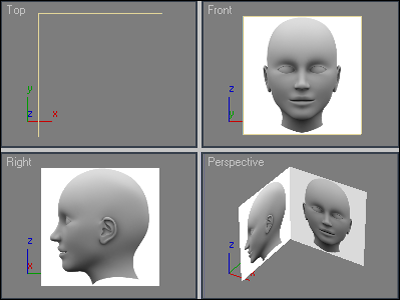
\includegraphics[width=6cm]{images/head_tut/1.png}}
  \quad
  \subfloat[Modelowanie warg.]{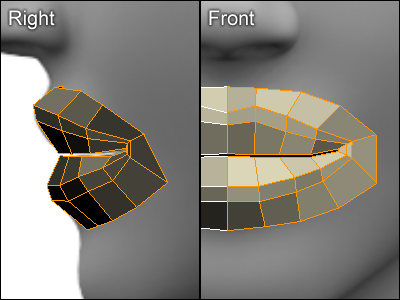
\includegraphics[width=6cm]{images/head_tut/4.png}}
  \label{mo_01}
  \caption[Modelowanie obiektów.]{Modelowanie obiektów~$^{\decimal{footnote}}$.}
\end{figure}
\begin{figure}[h]
  \centering
  \subfloat[Modelowanie policzków.]{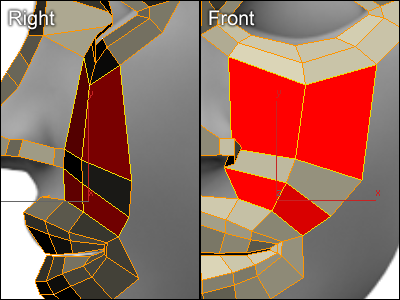
\includegraphics[width=6cm]{images/head_tut/6.png}}
  \quad
  \subfloat[Modelowanie nosa.]{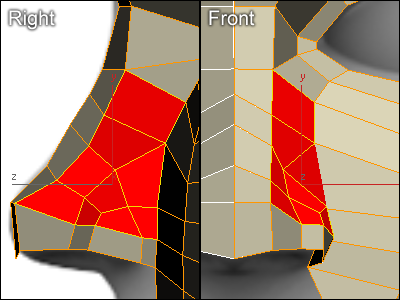
\includegraphics[width=6cm]{images/head_tut/7.png}}
  \label{mo_02}
  \caption[Modelowanie obiektów cd.]{Modelowanie obiektów~$^{\decimal{footnote}}$ cd.}
\end{figure}
\footnotetext[\value{footnote}]{Źródło:
\url{http://www.secondpicture.com/tutorials/3d/3d_modeling_of_a_human_head_3ds_max_01.html}} }

% !!!!!!! DORZUC JESZCZE TE OBRAZKI !!!!!!!!! po dwa w wierszu wystarczą 
%\begin{center}
%\begin{tabular}{c | c | c}
%  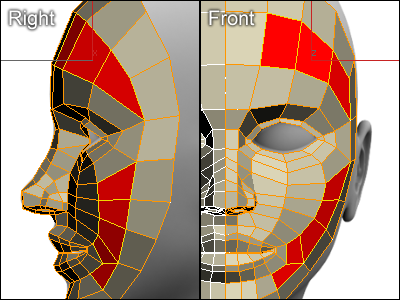
\includegraphics[width=4cm]{images/head_tut/9.png}
%  &
  %\caption{Wymodelowana twarz.}
%  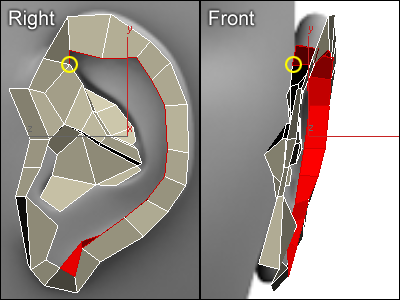
\includegraphics[width=4cm]{images/head_tut/11.png}
  %\caption{Modelowanie ucha.)&
%  &
 %\begin{figure}
%  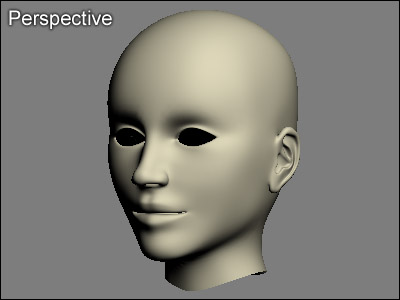
\includegraphics[width=4cm]{images/head_tut/12.png}
  %\caption{Finalny model po wygładzeniu.}
  %\end{figure}
%\end{tabular}
%\end{center}

\subsection{Modelowanie progresywne}
Jest to rozwinięcie zwykłego modelowania o wykorzystanie sekwencji obrazów
odniesienia zamiast pojedynczego tła. Proces tworzenia składa się z kilku
powtarzalnych kroków:
\begin{enumerate}
  \item oznaczenie nowych krawędzi obiektów;
  \item przejście do kolejnego ujęcia i ewentualne dodanie poprawek do
  naniesionych opisów krawędzi;
  \item powtórzenie kroków aż do uzyskania zadowalającego efektu.
\end{enumerate}

Niewątpliwą zaletą jest to, że podstawowy, nieskomplikowany model otrzymuje się
bardzo szybko. Model tworzy się poprzez generowanie siatki na obrazie
dwuwymiarowym, a dane przestrzenne są wyliczane automatycznie. Im więcej ujęć
jest dostępnych dla projektanta, tym lepsze efekty może osiągnąć. Z uwagi na to,
że algorytm bazuje na automatycznym wykrywaniu zmiany obrazu wymagane jest, aby
obrazy były dobrej jakości i w dobrym oświetleniu.
Kilka zrzutów ekranu z kolejnych kroków procesu tworzenia przykładowego modelu
zostało przedstawionych na ilustracjach \ref{progres1}, \ref{progres2},
\ref{progres3}, \ref{progres4}.

\addtocounter{footnote}{1}
\begin{figure}[h]
  \centering
  \subfloat[Modelowany obiekt]{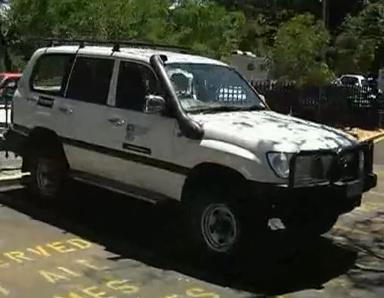
\includegraphics[width=6cm]{images/progr/1.png}\label{progres1}}
  \quad
  \subfloat[Początkowa struktura]{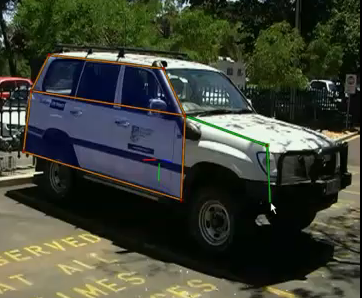
\includegraphics[width=6cm]{images/progr/2.png}\label{progres2}}
  \caption[Modelowanie progresywne.]{Modelowanie progresywne~$^{\decimal{footnote}}$.}
\end{figure}

\begin{figure}[h]
  \centering
  \subfloat[Struktura finalna]{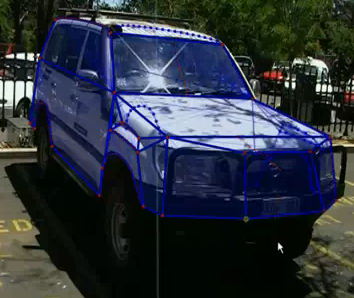
\includegraphics[width=6cm]{images/progr/3.png}\label{progres3}}
  \quad
  \subfloat[Wygenerowany obiekt]{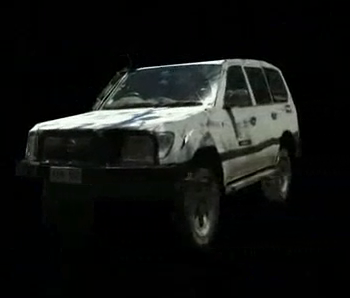
\includegraphics[width=6cm]{images/progr/4.png}\label{progres4}}
  \caption[Modelowanie progresywne cd.]{Modelowanie progresywne~$^{\decimal{footnote}}$cd.}
\end{figure}
\footnotetext[\value{footnote}]{Program
VideoTrace, \url{http://punchcard.com.au/wordpress/}}

\subsection{Modelowanie poprzez skanowanie}
Skanowanie jest to technika automatycznego tworzenia struktury oraz kolorów
trójwymiarowego modelu poprzez skanowanie powierzchni rzeczywistego modelu przy
użyciu specjalnych urządzeń. Urządzenia podczas skanowania tworzą chmurę
punktów, która później jest przetwarzana do dowolnego obsługiwanego formatu i
ewentualnie poddawana obróbce w programie modelującym. Technika skanowania jest
często używana, gdyż daje bardzo dokładne odwzorowanie obiektów. W zależności od
sposobu analizy struktury obiektu powstają pewne ograniczenia, jak np. problemy 
z powierzchniami, które charakteryzują się wysoką połyskliwością, problemy z
obiektami przeźroczystymi.

Skanery można podzielić na dwie grupy: odtwarzające kształt poprzez mechaniczny
kontakt oraz bezkontaktowe.

Skanery kontaktowe mają ograniczony zakres funkcjonalności z uwagi na to, że
wymagają fizycznego kontaktu z analizowanym obiektem, przez co obiekt może ulec
uszkodzeniu. Zaletą jest bardzo duża dokładność skanowania, natomiast wadą
jest powolność - z uwagi na mechaniczne przesuwanie sensora.

Skanery bezkontaktowe mają szerszy zakres używalności ponieważ nie niosą ze
sobą ryzyka uszkodzenia obiektu oraz, z uwagi na brak mechanicznego sensora,
mają o wiele większy zasięg i szybkość wykonywania skanowania. Ze względu na
sposób detekcji kształtu skanery tego typu dzielą się na aktywne i pasywne.
Skanery aktywne wysyłają jakiś typ promieniowania lub światła. Odległość do
obiektu może być wyliczana poprzez badanie czasu wędrówki wysłanych danych lub triangulując pozycje punktu lasera. Kształt może zostać
otrzymany również poprzez rzutowanie na obiekt ustalonego wzoru i jego ruch.
Detektor na podstawie zmiany rzutowanego wzoru względem oryginalnego odtwarza
kształt.
Skanery pasywne bazują na promieniowaniu istniejącym w środowisku (odbicie
światła, podczerwień) i nie emitują żadnych wiązek w kierunku obiektu. Do tej
grupy zaliczają się również skanery wyznaczające obrys z sekwencji obrazków,
gdzie obiekt jest umieszczony na tle o dużym kontraście.

\addtocounter{footnote}{1}
\begin{figure}[h]
  \centering
  \subfloat[Model
  1.]{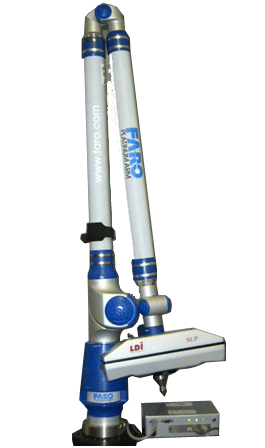
\includegraphics[width=4cm]{images/laser_scanner.png}\label{skan1}}
  \quad
  \subfloat[Model 2.]{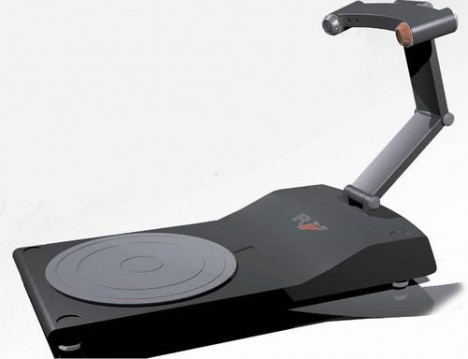
\includegraphics[width=6cm]{images/laser_scanner2.jpg}\label{skan2}}
  \caption[Lserowe skanery 3D]{Laserowe skanery 3D~$^{\decimal{footnote}}$.}
\end{figure}
\footnotetext[\value{footnote}]{Źródła:
\url{http://www.laserdesign.com/products/scanners_and_software/portable_laser_scanners/surveyor_fa-series/},
\url{http://www.coolest-gadgets.com/20090202/real-view-3d-scanner/}}

%\subsection{Modelowanie z wykorzystaniem wymiarowania}

%\subsection{Generowanie obiektów}
%\subsubsection{Modelowanie proceduralne}
%\subsubsection{Generowanie obiektu z wykorzystaniem gramatyki kształtu}
\subsection{Generowanie obiektu z wykorzystaniem gramatyki kształtu}
Tworzenie obiektów z użyciem gramatyk kształtu jest tematem dalszej części tej
pracy. Technika ta wykorzystuje opis struktury kształtu obiektu i relacji
pomiędzy jego elementami składowymi.
    \newpage
    \section{Kilka słów o gramatykach}
Głównym celem pracy jest opracowanie gramatyki kształtu twarzy ludzkiej,
powinniśmy więc na samym początku dowiedzieć się czym właściwie jest ta
gramatyka kształtu.

Gramatyka jest ,,działem językoznawstwa zajmujący się badaniem reguł, które
rządzą generowaniem wyrazów i zdań języka''~\cite{wiki01}. Jak widać definicja
ta jest ściśle związana z lingwistyką, ale interesujące w tej definicji jest ,,badanie reguł'' oraz ,,generowanie wyrazów i zdań''.
Jeżeli tymi wyrazami są jakieś figury geometryczne (kształty) 2D bądź 3D:

\begin{figure}[h!]
\centering
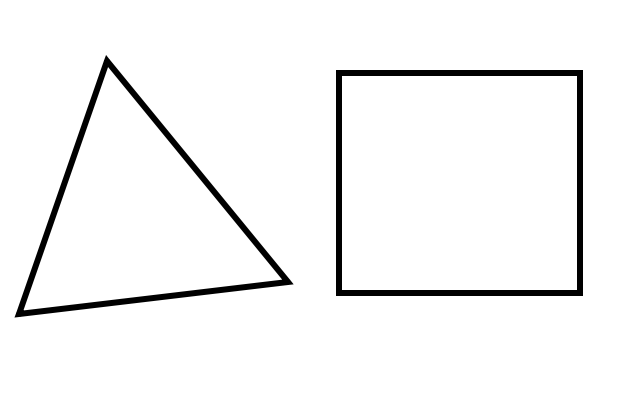
\includegraphics[width=6cm]{images/ksztalt.png}
\caption{Przykład podstawowych kształtów (źródło własne)}
\end{figure}
to regułami będą przekształcenia tych figur takie jak np. obrót, przesunięcie.

\begin{figure}[h!]
\centering
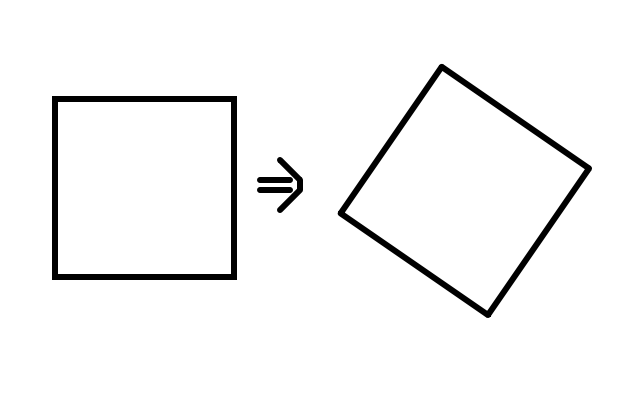
\includegraphics[width=6cm]{images/obrot.png}
\caption{Obrót kształtu (źródło własne)}
\end{figure}

Tak jak w językach wyrazy, tak i tu kształty mogą być dowolne, nawet bardzo
skomplikowane.
To skoro podstawowe kształty mogą być dowolnie skomplikowane to po co ta cała
gramatyka? Odpowiedź jest prosta - po co wymyślać wyrazy w języku, które
określają coś skomplikowanego jeśli można to opisać {\em zdaniem}. Czym w takim
razie jest zdanie? Jest to nic innego jak zbiór wyrazów połączonych
odpowiednimi regułami. I właśnie dzięki tym regułom możemy tworzyć
skomplikowane kształty.

W dalszej części rozdziału zostaną matematycznie przedstawione podstawowe
gramatyki wykorzystywane w grafice komputerowej (źródło~\cite{gaudi}). Jako
wprowadzenie do gramatyk kształtu można wykorzystać przykład prostej gramatyki, za pomocą
której możemy wygenerować strukturę butelki coca coli~\cite{link10}. Bazując na
zdjęciach różnych modeli butelki~\ref{coca_cola} można łatwo określić jej
logiczną budowę oraz utworzyć odpowiedni parametryczny kształt.

\addtocounter{footnote}{1}
\begin{figure}[h!]
\centering
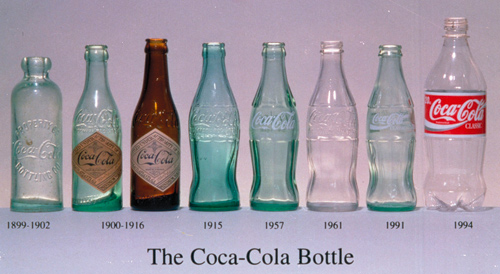
\includegraphics[width=14cm]{images/Coca-Cola.jpg}
\caption[Wybrane butelki napoju Coca Cola na przestrzeni
lat.]{Wybrane butelki napoju Coca Cola na przestrzeni
lat~$^{\decimal{footnote}}$.}
\label{coca_cola}
\end{figure}
\footnotetext[\value{footnote}]{\url{http://www.redesign-day.com/design-icons-the-coca-cola-bottle/}}

\begin{figure}[h!]
\centering
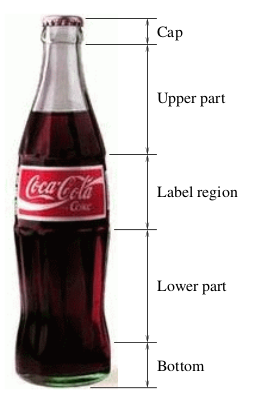
\includegraphics[width=5cm]{images/coca-cola_parts.png}
\caption{Podział butelki Coca Cola na logiczne części.~\cite{link10}}
\label{coca_cola_parts}
\end{figure}

Mając wydzielone logiczne części możemy rozpisać gramatykę kształtu zaczynając
od początkowego symbolu $*I$ poprzez kolejne $*U$ -- górna część, $*D$ -- dolna
część, $*T$ -- nakrętka.

\begin{figure}[h!]
\centering
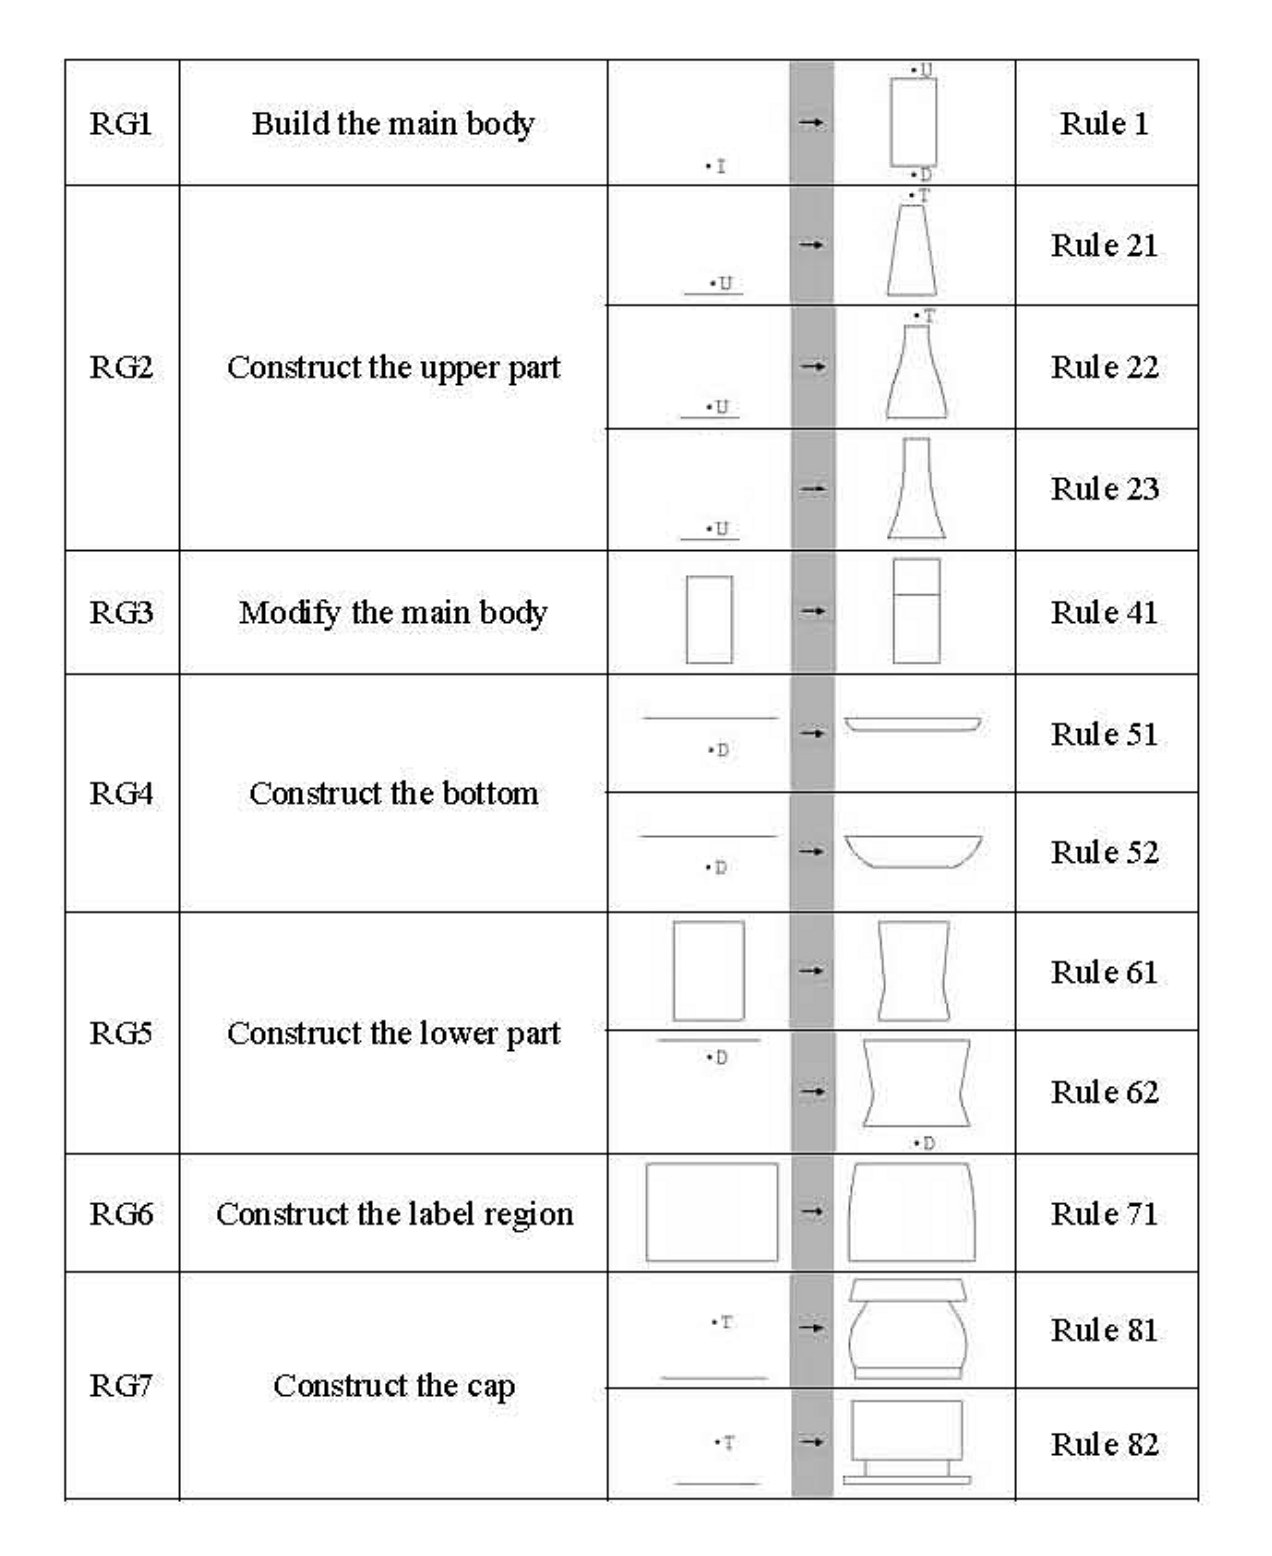
\includegraphics[width=12cm]{images/table01.png}
\caption{Reguły gramatyki kształtu do wygenerowania butelek
coca-coli.~\cite{link10}}
\label{coca-cola_regules}
\end{figure}

Przykład rozpisywania gramatyki od symbolu początkowego poprzez reguły aż do
uzyskania gotowych butelek znajduje się na ilustracji~\ref{coca_cola_create},
oraz wygenerowane wszystkie możliwe butelki z wykorzystaniem reguł
z~\ref{coca-cola_regules} znajduje się na ilustracji~\ref{coca_cola_all}.


\begin{figure}[h!]
\centering
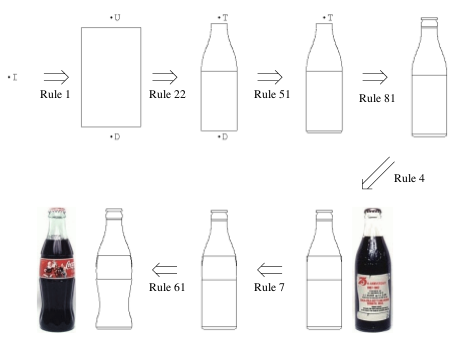
\includegraphics[width=9cm]{images/coca-cola_create.png}
\caption{Przykład generowania butelki na podstawie gramatyki
kształtu~\cite{link10}.}
\label{coca_cola_create}
\end{figure}

\begin{figure}[h!]
\centering
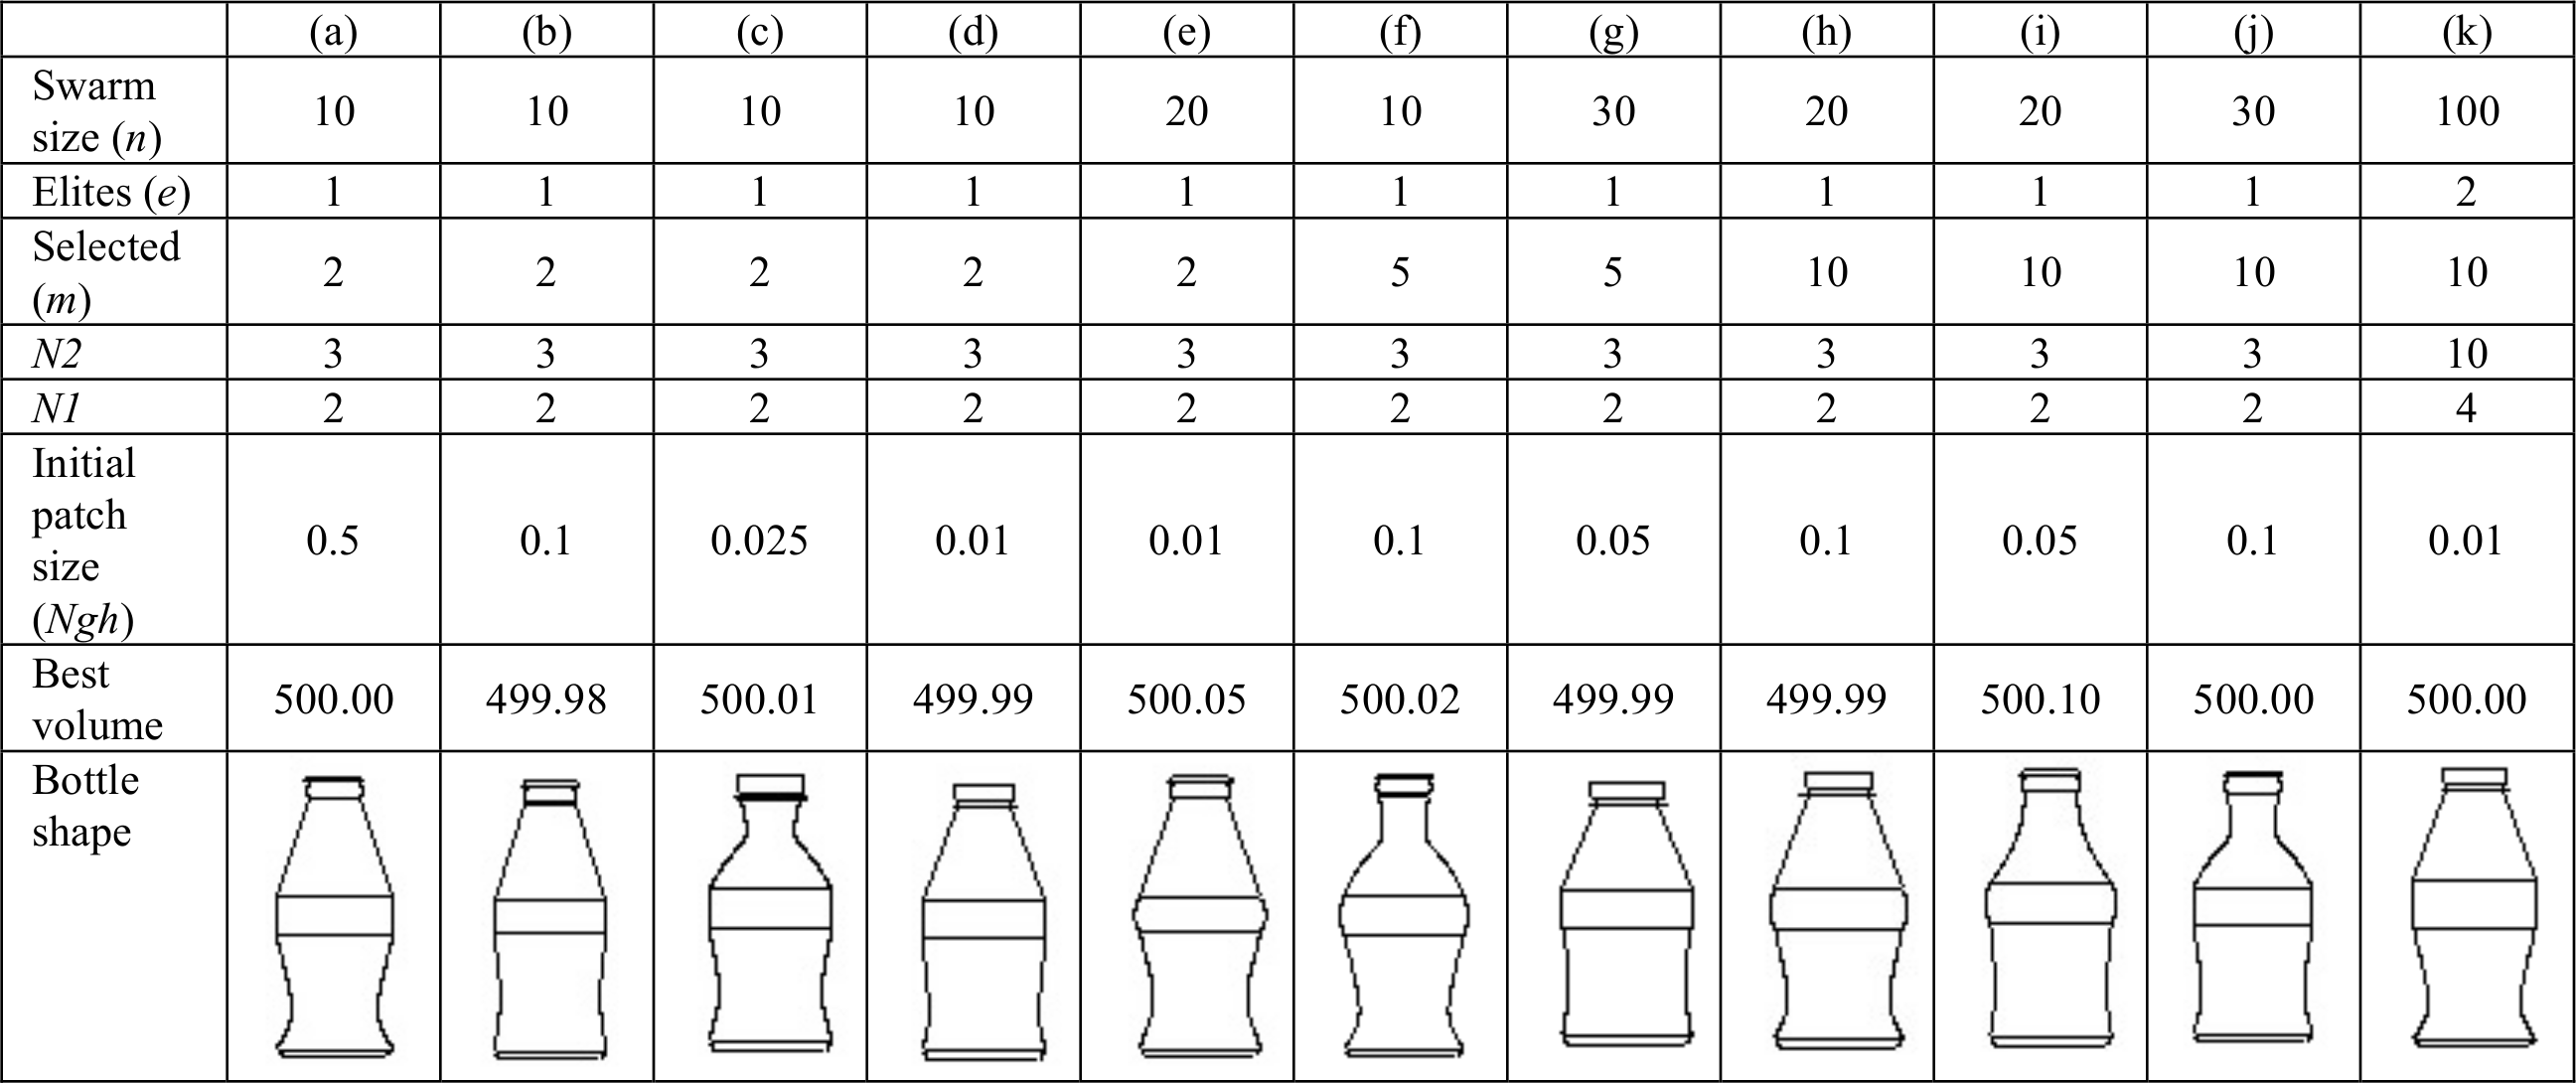
\includegraphics[width=15cm]{images/bootles.png}
\caption{Wygenerowane butelki na podstawie reguł~\cite{link10}}
\label{coca_cola_all}
\end{figure}

\subsection{Gramatyka formalna}
Gramatyka kształtu wywodzi się od gramatyki formalnej, dzięki której można
opisać skomplikowane struktury korzystając z podstawowych elementów.
Główną zaletą jest jej prostota i czytelność. Jest zatem doskonałym narzędziem
do grupowania elementów podobnych oraz ich generowania używając prostszych
części. W dalszej części zostaną matematycznie przedstawione gramatyki formalne.
Rozpocznijmy więc od definicji gramatyki formalnej -- ,,sposób opisu {\em języka
formalnego}, czyli podzbioru zbioru wszystkich słów skończonej długości nad
danym alfabetem''~\cite{wiki02}.

\subsubsection{Podstawowe pojęcia}
\begin{description}
 \item[Język formalny] podzbiór zbioru wszystkich {\em słów} nad pewnym {\em
alfabetem};
 \item[Alfabet] jest to niepusty, skończony zbiór symboli, np.:\\
$T1 = \{a, b, c,\ldots, x, y, z\}$ - alfabet łaciński;\\
$T2 = \{0,1\}$ - alfabet binarny;
 \item Niech $T$ będzie alfabetem, wtedy:\\
$T \neq \emptyset$, $\#T < \infty$\qquad ($\#T$ -- moc zbioru $T$);
 \item[Symbol] pojęcie nie definiowalne (synonimy: znak, litera);
 \item[Słowo] (synonim: łańcuch, wyraz) skończony ciąg zestawionych razem
symboli alfabetu;\\
Rekurencyjna definicja łańcucha nad alfabetem $T$:
  \begin{enumerate}
    \item jest łańcuchem nad $T$ ($\epsilon$ -- łańcuch pusty, niezawierający
    żadnego znaku);
    \item jeśli $x$ jest łańcuchem nad $T$ i $a \in T$ to $xa$ jest łańcuchem
    nad $T$;
    \item nic innego nie jest łańcuchem poza tym, co wynika z punktów (1) i (2).
  \end{enumerate}
 \item[Językiem] $L$ nad alfabetem $T$ nazywamy dowolny podzbiór $L$ zbioru
$T^*$, gdzie $T^*$ jest zbiorem wszystkich łańcuchów nad alfabetem $T$:
  \begin{equation}
  L \subseteq T^*
  \vspace{-10pt}
  \end{equation}
 \item Przykłady języków:
  \begin{description}
   \item[$L_0 = \emptyset$]-- język pusty;
   \item[$L_1 = \{\epsilon\}$]-- język zawierający tylko słowo puste;
   \item[$L_2 = T^*$]-- język zawierający wszystkie słowa nad alfabetem $T$;
   \item[$L_3 = \{\epsilon, 0, 01, 001\}$]-- język zawierający skończoną liczbę
  słów;
   \item[$L_4 = \{0, 01, 011, \ldots\} = \{01^n | n \ge 0\}$]-- język
  nieskończony.
  \end{description}
 \item[Gramatyka] $G$ nazywamy uporządkowaną czwórkę:
  \begin{equation}
  G = <N, T, P, Z>
  \vspace{-10pt}
  \end{equation}
 gdzie:
  \begin{description}
   \item[$N$]-- zbiór symboli nieterminalnych;
   \item[$T$]-- zbiór symboli terminalnych;
   \item[$P$]-- zbiór produkcji, z których każda ma postać
  $\alpha\rightarrow\beta$;
   \item[$Z\in N$]-- wyróżniony symbol początkowy (nieterminalny).
  \end{description}
 przy czym:
  \begin{description}
   \item[$P\subseteq (N\cup T)^+\times(N\cup T)^*$]
   \item[$P=\{\alpha\rightarrow\beta | \alpha\in(N\cup T)^+, \beta\in(N\cup
  T)^*\}$]
  \end{description}
 \item[Wyprowadzalność.] Słowo $\psi$ jest wyprowadzalne bezpośrednio ze słowa
$\omega$ w gramatyce G, co zapisujemy:
  \begin{equation}
  \omega \Longrightarrow_G \psi
  \vspace{-10pt}
  \end{equation}
jeśli:
  \begin{description}
   \item $\omega = \gamma\alpha\delta$;
   \item $\psi = \gamma\beta\delta$;
   \item $(\alpha\rightarrow\beta)\in P$;
   \item $\alpha,\beta,\gamma,\omega,\psi\in(N\cup T)^*$.
  \end{description}
Słowo $\psi$ jest wyprowadzane ze słowa $\omega$ w gramatyce $G$, co zapisujemy:
  \begin{description}
   \item $\omega \Longrightarrow_G^+\psi$
jeżeli istnieja $\varphi_0$, $\varphi_1$,\ldots,$\varphi_n\in(N\cup T)^*$
takie, że:
   \item $\varphi_0 = \omega$,
   \item $\varphi_n = \psi$,
   \item $\varphi_i-1 \Longleftrightarrow \varphi_i$,  $i = 1,2,\ldots,n$
  \end{description}
Sekwencje $\varphi_0$,$\varphi_1$,\ldots,$\varphi_n$ nazywamy wyprowadzeniem o
długości $n$.
Definiujemy ponad to:
  \begin{description}
   \item
$(\omega\Longrightarrow^*\psi)\Longleftrightarrow(\omega\Longrightarrow^+)\vee(\omega=\psi)$
  \end{description}
Relacje $\Longrightarrow^+$ oraz $\Longrightarrow^*$ są odpowiednio przechodnim
oraz przechodnim i zwrotnym domknięciem relacji bezpośredniej wyprowadzalności
$\Longrightarrow$. Jeżeli wiadomo, o jaką gramatykę chodzi, pomijamy dolny
indeks ,,G'' w oznaczeniu tych relacji pisząc po prostu: $\Longrightarrow^+$,
$\Longrightarrow^*$.
 \item[Jezyk.] Gramatyka jest jednym ze sposobów definiowania języka formalnego.
Mając daną gramatykę $G$ oznaczamy przez $L(G)$ zbiór wszystkich słów, które
mogą być w tej gramatyce wyprowadzone z symbolu początkowego $Z$. Zbiór ten
nazywamy językiem generowanym przez daną gramatykę:
  \begin{description}
   \item $L(G)={x\in T^*|Z\Longrightarrow^*x}$
  \end{description}
Aby zilustrować tą definicję, rozważmy gramatykę:
  \begin{description}
   \item $G=<N,T,P,S>$
  \end{description}
gdzie:
  \begin{description}
   \item $N={S,A,B}$
   \item $T={a,b,c}$
   \item $P={S\longrightarrow cAb, A\longrightarrow aBa, B\longrightarrow aBa,
B\longrightarrow cb}$
  \end{description}
Gramatyka ta generuje język $L(G)={ca^ncba^nb|n\geq 1}$
Dla przykładu: aby wygenerować słowo $caacbaab$ dla $n=2$ należy zastosować
nastepującą sekwencję produkcji:
  \begin{description}
   \item $S\longrightarrow cAb\longrightarrow caBab\longrightarrow
caaBaab\longrightarrow caacbaab$
  \end{description}
\end{description}
Noam Chomsky~\cite{chomsky} zdefiniował cztery klasy gramatyk oraz cztery klasy
języków formalnych:
 \begin{enumerate}
  \item gramatyki klasy 0 lub gramatyki nieograniczone (unrestricted). Produkcje
  w tego rodzaju gramatykach mają postać $\alpha\longrightarrow\beta$, gdzie
  $\alpha$ i $\beta$ są dowolnymi łańcuchami symboli tej gramatyki, przy czym
  $\alpha\neq\epsilon$. Nie nakłada żadnych ograniczeń na postać produkcji
  gramatyki w stosunku do ogólnej definicji gramatyki. Języki generowane przez
  gramatyki tego typu noszą nazwę {\em języków rekurencyjnie przeliczalnych};
  \item gramatyki klasy 1 lub gramatyki kontekstowe. Produkcje mają postać
  $\alpha\longrightarrow\beta$, gdzie $\alpha$ i $\beta$ są takimi łańcuchami
  tej gramatyki, ze łańcuch $\beta$ jest przynajmniej tak długi jak łańcuch
  $\alpha$ oraz dodatkowo dopuszczona jest produkcja $Z\longrightarrow\epsilon$,
  jeśli język zawiera słowo puste. Języki generowane przez tego typu gramatyki
  nazywane są {\em językami kontekstowymi};
  \item gramatyki klasy 2 lub gramatyki bezkontekstowe. Produkcje mają postać
  $A\longrightarrow\beta$, gdzie $A$ jest nieterminalem $(A\in N)$, zaś łańcuch
  $\beta$ jest dowolnym łańcuchem symboli tej gramatyki. Języki generowane przez
  tego typu gramatyki noszą nazwę {\em języków bezkontekstowych};
  \item gramatyki klasy 3 lub gramatyki regularne. Jeśli produkcje mają postać
  $A\longrightarrow xB$ lub $A\longrightarrow x$, gdzie $A$ i $B$ są
  nieterminalami $(A,B\in N)$, zaś łańcuch $x$ jest dowolnym łańcuchem symboli
  terminalnych tej gramatyki $(x\in T^*)$, to gramatykę taką nazywamy {\em
  gramatyką prawostronnie liniową}. Jeśli produkcje mają postać
  $A\longrightarrow Bx$ lub $A\longrightarrow x$, gdzie $A$ i $B$ są
  nieterminalami $(A,B\in N)$, zaś łańcuch $x$ jest dowolnym łańcuchem symboli
  terminalnych tej gramatyki $(x\in T^*)$, to gramatyki takie nazywamy {\em
  gramatykami lewostronnie liniowymi}.
\end{enumerate}
\subsection{Gramatyki stochastyczne}
Gramatyki stochastyczne są rozszerzeniem gramatyk łańcuchowych. Wprowadza się w
nich czynnik probabilistyczny. Oznacza to, że każda reguła jest powiązana z
pewnym prawdopodobieństwem, przy czym suma prawdopodobieństw wystąpienia reguł o
tych samych lewych stronach wynosi 1. Wybór produkcji do zastosowania w kolejnym
kroku procesu derywacji, realizowany jest poprzez losowanie z uwzględnieniem
czynnika prawdopodobieństwa, które może być zmieniane w całym procesie (na
przykład po wykonaniu reguły zmniejsza się jej czynnik).

Dla prostoty zapisu rozpatrzmy gramatyki bezkontekstowe. Analogicznie definicja
ta może być przedstawiona dla różnych klas gramatyk. Każda produkcja
$\alpha\longrightarrow\beta$ będzie miała postać $A\longrightarrow X_ij$, gdzie
$X_ij$ będzie łańcuchem stworzonym z nieterminali i terminali.
\\
Rozpatrzmy gramatykę:
\begin{equation}
G=<N,T,P,S>,
\vspace{-10pt}
\end{equation}
gdzie:
\begin{description}
\item $N={A_1, A_2, \ldots, A_m}$,
\item $A_1\longrightarrow X_{11}, A_2\longrightarrow X_{12}, \ldots,
A_n\longrightarrow X_{1n}, \ldots,$
\item $A_m\longrightarrow X_{m1}, A_m\longrightarrow X_{m2}, \ldots,
A_m\longrightarrow X_{mn}$, przy czym $X_{ij}\in (N\times T)^+$
\end{description}
Stochastyczną (bezkontekstową) gramatyką jest czwórka:
\begin{equation}
G_S=<N,T,P^S,S>
\vspace{-10pt}
\end{equation}
gdzie $N$, $T$ oraz $S$ są definiowane jak dla zwykłych gramatyk
bezkontekstowych, zaś $P^S$ jest zbiorem produkcji postaci
$(A_i\longrightarrow X_{ij},p_{ij})$, takim że $A_i\in N$, $X_{ij}\in (N\times
T)^+$ oraz $\displaystyle\sum_{j=0}^{n_i}p_{ij}=1$, dla $i=1,\ldots,m$, gdzie
$n_i$ oznacza liczbę produkcji, których lewa strona ma postać $A_i$.
Zapis dwóch produkcji o tych samych lewych stronach, ale o różnych
prawdopodobieństwach można przedstawić następująco:
\begin{enumerate}
  \item $S\longrightarrow AB : 0.3$
  \item $S\longrightarrow BA : 0.7$
\end{enumerate}
Taki zapis oznacza, że prawdopodobieństwo wykonania pierwszej produkcji jest
równe $0.3$, a drugiej produkcji $0.7$ w pojedynczym kroku przepisywania.
\subsection{Gramatyki wielowymiarowe}
Dotychczas opisane gramatyki dotyczyły wyłącznie jednowymiarowej przestrzeni,
gdzie jedyną relacją pomiędzy sąsiednimi symbolami w łańcuchu była konkatenacja.
Jeśli chodzi o zastosowanie tych gramatyk w grafice komputerowej, to jest ono
bardzo ograniczone, dlatego też stworzono na ich bazie gramatyki wielowymiarowe.
Poniżej zostaną opisane poszczególne rodzaje gramatyk wielowymiarowych.
\subsubsection{Gramatyki tablicowe}
Gramatyki tablicowe~\cite{chanda} są analogiczne do gramatyk łańcuchowych z
tym, że używane są do generowania bardziej skomplikowanych sekwencji symboli w dwu lub więcej
wymiarowej przestrzeni. Produkcje mają postać dwuwymiarowych wzorców osadzonych
na siatce zamiast liniowej sekwencji, jak to ma miejsce w jednowymiarowych
gramatykach. Cały łańcuch jest modelowany jako funkcja odwzorowywująca zbiór pól
na siatce w zbiór symboli terminalnych gramatyki oraz symbolu pustego (\#).
Pojęcie {\em łączności} dla tego typu łańcuchów jest zdefiniowane w oparciu o
współrzędne symbolu na siatce. Dwa punkty $(i,j)$ i $(h,k)$ są sąsiadami, czyli
są połączone jeśli $|i-h|+|j-k|=1$.
Tablica $\Sigma$ jest nazywana {\em złączoną}, jeśli dla wszystkich symboli
$A,B$ w tej tablicy, za wyjątkiem symboli pustych (\#), istnieje sekwencja
$A=A_0,A_1,A_2,\ldots,A_n=B$ symboli, różnych od symbolu pustego (ścieżka) taka,
że $A_i$ jest sąsiadem $A_{i-1}$. Definicja jasno określa, że wszystkie symbole
puste są ze sobą połączone. Nakłada się również pewne ograniczenia na to, w jaki
sposób definiowane są reguły. Mianowicie, reguły posiadają strukturę gramatyki
izometrycznej. Dla takiej gramatyki, dla każdej reguły
$\alpha\longrightarrow\beta$, długość $\alpha$ i $\beta$ musi być taka sama.
Przy takim ograniczeniu, generowany łańcuch zawsze będzie miał skończoną długość
(w początkowej konfiguracji), zatem także liczba możliwych łańcuchów będzie
skończona.

Jakkolwiek język gramatyki izomatrycznej $G$ jest zdefiniowany jako
zbiór terminalnych łańcuchów $\tau$, takich że nieskończony łańcuch
$\#^\infty\tau\#^\infty$ może być otrzymany w gramatyce $G$ z początkowego
łańcucha $\#^\infty S\#^\infty$. W związku z tym, włączając regułę zawierającą
znak ,,*'' otrzymujemy zmienną długość łańcucha.

W gramatykach tablicowych startujemy z nieskończoną dwuwymiarową tablicą
zawierającą symbole puste (\#) z początkowym symbolem na którejś z pozycji.
Każda reguła zastępuje jedną tablicę inną. Reguły powinny spełniać warunki
izometryczne w przeciwnym razie nie będzie jasne jak zamienić większą tablicę na
mniejszą i odwrotnie, utrzymując przy tym łączność.

Poniżej~\ref{g_tab} przedstawiony został przykładowy zbiór reguł gramatyki
tablicowej oraz wyprowadzienie przykładowego słowa.

\begin{figure}[h]
  \centering
  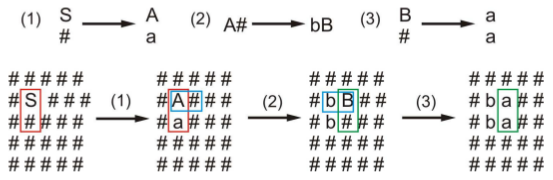
\includegraphics{images/g_tab.png}
  \caption{Proces generowania słowa w gramatykach tablicowych.~\cite{gaudi}}
  \label{g_tab}
\end{figure}

\subsubsection{Gramatyki grafowe.}
Łańcuchy oraz tablice mogą być rozpatrywane również jako specyficzne struktury
grafowe. Gramatyki grafowe są uogólnieniem gramatyk łańcuchowych na
grafy~\cite{chanda}. Liczba relacji pomiędzy sąsiadami może posiadać przypadkowe
wartości (zamiast 2 dla gramatyk łańcuchowych i 4 dla tablicowych). Proces tworzenia słowa za pomocą
gramatyki grafowej oparty jest o rozpoznawanie konkretnych podgrafów oraz ich
zastępowaniu zgodnie z produkcjami. Zatem, dla każdej reguły postaci
$\alpha\longrightarrow\beta$, $\alpha$ i $\beta$ powinny być reprezentowane
przez podgrafy i ich zamiana powinna polegać na tym, że $\alpha$ zostanie
usunięte z całego grafu i zastąpione przez $\beta$. Szczególnym przypadkiem
gramatyk tego rodzaju są gramatyki drzewiaste, których językiem (zbiorem
generowanych słów) jest zbiór struktur drzewiastych. Poniżej został
przedstawiony przykładowy zbiór reguł oraz przykładowy graf przez ten zbiór
wygenerowany~\ref{g_graf}.

\begin{figure}[h]
  \centering
  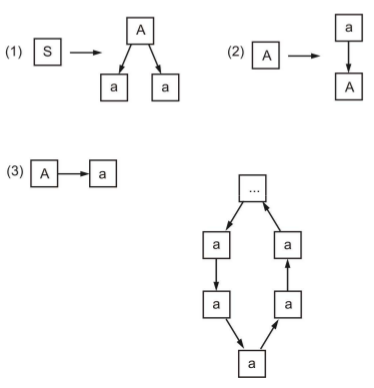
\includegraphics{images/g_graf.png}
  \caption{Przykład gramatyki grafowej, oraz wygenerowany przez nią
  graf.~\cite{gaudi}}
  \label{g_graf}
\end{figure}

\subsection{Gramatyki równoległe.}
Przedstawione wcześniej gramatyki wykorzystują model sekwencyjny zastępowania
symboli nieterminalnych. Jak wcześniej wspomniano mówimy, że gramatyka
$G=<N,T,P,S>$ akceptuje słowo $x$ jeśli istnieje ciąg takich produkcji:
\begin{equation}
X_0,X_1,\ldots,X_k:S\longrightarrow X_0\longrightarrow
X_1\longrightarrow\ldots\longrightarrow X_k=x,
\vspace{-10pt}
\end{equation}
gdzie każdy krok ($\longrightarrow$) oznacza zastąpienie tylko jednego elementu
prawej strony produkcji. W przypadku gramatyk równoległych, wprowadzono
dodatkowy warunek. Mówimy, że gramatyka równoległa (oznaczana dalej jako
$G^{||}$) akceptuje słowo $x$, jeśli istnieje taki ciąg równoległych produkcji
$X_0,X_1,\ldots,X_k:S\Longrightarrow X_0 \Longrightarrow
X_1\Longrightarrow\ldots\Longrightarrow X_k=x$ taki, że każdy krok iteracji
($\Longrightarrow$) oznacza wykonanie wszystkich możliwych zastąpień elementów
prawej strony. Efektem tego jest fakt, że języki akceptowane przez gramatyki
równoległe i równoważne im gramatyki sekwencyjne (wyłączając niektóre proste
przypadki) różnią się.
Rozważmy następujący przykład: mamy kolejne dwie produkcje: $S\longrightarrow
SS$, $S\longrightarrow a$, wtedy języki akceptowane przez te gramatyki wyglądają
następująco:
\begin{equation}
L(G)={a^n,n\geq 1}\\
L(G)={a^{2n},n\geq 1}
\vspace{-10pt}
\end{equation}
Tak więc w rzeczywistości język $L(G^{||})$ nie jest bezkontekstowy, mimo że
oparty jest na gramatyce bezkontekstowej. W przypadku gramatyk regularnych (po
prawej stronie produkcji występuje maksymalnie jeden terminal) języki przez nie
generowane są równoważne.

%% jakis kod

Gramatyki równoległe są wykorzystywane w grafice komputerowej przy realizacji
aplikacji opartych na systemach Lindenmeyera~\cite{lindenmeyer}. Te zostaną
omówione w kolejnej części rozdziału. Zalety stosowania tego podejścia są wielorakie: równoległość
daje, w przypadku dużych gramatyk możliwość rozproszenia aplikacji, przez co
uzyskujemy wysoką skalowalność i wydajność systemu. Ponadto fakt realizacji
wszystkich występujących w produkcji nieterminali w taki sam sposób pozwala na
uzyskanie w prosty sposób regularności tworzonego słowa.

\subsection{L-systemy.}
L-systemy (systemy Lindenmeyera)~\cite{lindenmeyer} początkowo stworzone zostały
na potrzeby symulacji wzrostu roślin w grafice komputerowej. Znalazły również zastosowanie w
generowaniu fraktali. Są one szczególnym przypadkiem automatów gramatyki
równoległej. Produkcje, jak w gramatykach łańcuchowych, stosuje się iteracyjnie
z góry określoną ilość razy, począwszy od pewnego stanu początkowego, zaś zbiory
reguł są stosunkowo małe.

Szczególnym przypadkiem L-systemów są systemy D0L (deterministyczne i
bezkontekstowe L-systemy). Charakteryzują się tym, że dla każdego nieterminala
mamy tylko jedną regułę, którą możemy zastosować. W przypadku, gdy istnieje
więcej produkcji możliwych do zastosowania dla pojedynczego terminala, oraz dla
każdej z nich przypisane jest jakieś prawdopodobieństwo to taki L-system
nazywamy stochastycznym.

Najbardziej popularnym i jednym z najbardziej rozpowszechnionych i
rozpoznawalnych języków programowania korzystających m.in. z idei L-systemów
jest język Logo. Oparty jest on na idei żółwia, którego ruchy definiuje
programista za pomocą prostych rozkazów (podniesienie, opuszczenie pisaka,
przesunięcie o określoną odległość w przód czy w tył, obrót żółwia o określony
kąt) z możliwością ich agregacji w procedury.

W najprostszych L-systemach stosuje się trzy sposoby zapisu gramatyki:
literalny, graficzny i proceduralny. Alfabet zapisu literalnego~\ref{fractal01}
opiera się na dwóch symbolach nieterminalnych: ,,F'' -- ruch w przód kursora,
,,-'' -- podnieś pisak i ,,+'' -- opuść. Za pomocą tych trzech symboli
definiowany jest symbol początkowy oraz produkcje. Drugim zapisem jest zapis
graficzny~\ref{fractal02}. Składa się on z dwóch części: symbolu początkowego
(inicjatora) oraz reguły (generatora), a sam proces generowania słowa przebiega
analogicznie jak w przypadku zapisu literalnego. Trzeci rodzaj zapisu jest zapis
proceduralny, realizowany np. przez wcześniej wspomniany język Logo.

L-systemy, w których stosuje się interpretacje żółwia umożliwiają tworzenie
bardzo zróżnicowanych obiektów, w tym przede wszystkim fraktale. Fraktale
charakteryzują się wysokim stopniem podobieństwa niezależnie od stopnia
złożoności, skali oraz fragmentu fraktala, który się obserwuje. Wraz ze wzrostem
(ilością wykonywanych iteracji) otrzymuje się ciekawsze kształty. Są proste do
tworzenia, ponieważ wymagają stosunkowo małego zbioru reguł (zwykle 1,2), a dają
bardzo dobre efekty graficzne. Większość z nich opiera się na zapisie
łańcuchowym, a symbole tworzące ostatni łańcuch interpretowane są np.: na ruchy
kursora (zgodnie z gramatyką żółwia). Przykładem takiego fraktala są np.: krzywa
Kocha, lub płatek śniegu. Proces budowy fraktali rozpoczyna się zazwyczaj od
prostego kształtu inicjującego, który w zapisie graficznym reprezentuje np.:
odcinek bądź łamaną, oraz jednej lub dwóch reguł, które są stosowane do każdego
symbolu w już wygenerowanym łańcuchu.

\addtocounter{footnote}{1}
\begin{figure}[h!]
  \centering
  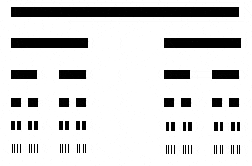
\includegraphics{images/fractal.png}
  \caption[Zbiór Cantora. F -- symbol początkowy, F-F+F --
  generator]{Zbiór Cantora. F -- symbol początkowy, F-F+F --
  generator~$^{\decimal{footnote}}$.}
  \label{fractal01}
\end{figure}
\footnotetext[\value{footnote}]{\url{http://pl.wikipedia.org/wiki/Zbi\%C3\%B3r\_Cantora}}
\addtocounter{footnote}{1}
\begin{figure}[h!]
  \centering
  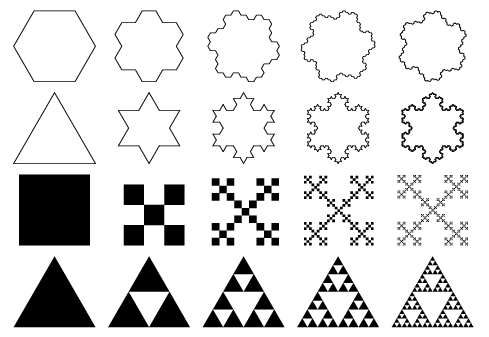
\includegraphics[width=11cm]{images/fractals.png}
  \caption[Inne przykłady fraktali]{Inne przykłady
  fraktali~$^{\decimal{footnote}}$.}
  \label{fractal02}
\end{figure}
\footnotetext[\value{footnote}]{\url{https://picasaweb.google.com/110433414991788678333/Fractals?fgl=true&pli=1}}

Początkowo działanie L-systemów w grafice było ograniczone do przestrzeni
dwuwymiarowych, jednak z czasem rozszerzono tą ideę do przestrzeni
trójwymiarowych (wprowadzono m.in. symbole rotacji względem dwóch pozostałych
osi).

Prusinkiewicz i Lindenmeyer w swojej pracy pod tytułem ,,The Algorithmic Beauty
of Plants''~\cite{abop} przedstawili możliwości wykorzystania L-systemów w
generowaniu modeli roślin (krzewów, drzew, kwiatów). Poszerzyli oni
funkcjonalność istniejącego systemu głównie poprzez dodanie trzeciego wymiaru,
sparametryzowanie gramatyki oraz dodanie tzw. procesu rozgałęziania poprzez
zastosowanie stosu do przechowywania aktualnego stanu kursora (pozycji,
kierunku, koloru oraz grubości rysowanej linii). Modyfikacje te pozwoliły
odwzorować naturalny dla świata roślin proces wzrostu.

Na ilustracji~\ref{fractal03} przedstawiony został przykład efektu rozgałęzienia
dla gramatyk dwuwymiarowych. W notacji literalnej takiego systemu odłożenie
aktualnego stanu kursora na stos używa się nawiasów kwadratowych.

\begin{figure}[h!]
  \centering
  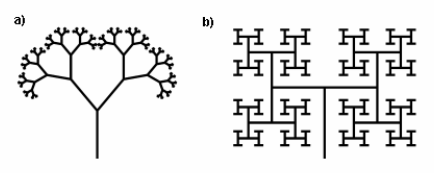
\includegraphics{images/fractal03.png}
  \caption{Fraktal drzewo dla kątów a) 30$^o$, b) 90$^o$.\cite{gaudi}}
  \label{fractal03}
\end{figure}

Zastosowania L-systemów są różnorakie, od tworzenia prostych kształtów
dwuwymiarowych i fraktali, poprzez generowanie trójwymiarowych obiektów i tworów
botanicznych, po tworzenie form graficznych na podstawie muzyki.

\begin{figure}[h!]
  \centering
  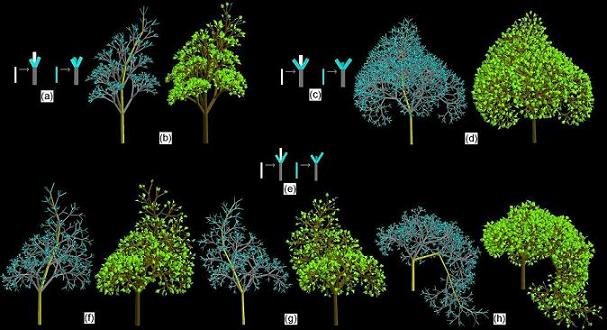
\includegraphics[width=12cm]{images/l-system01.jpg}
  \caption{Produkcje oraz wygenerowane za ich pomocą drzewa~\cite{ls01}.}
  \label{l-system01}
\end{figure}

\begin{figure}[h!]
  \centering
  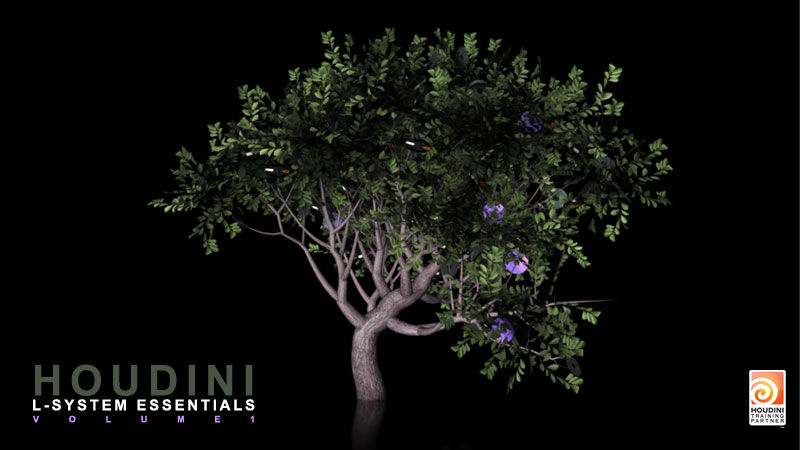
\includegraphics[width=10cm]{images/l-system02.jpg}
  \caption{Inny przykład wygenerowanego trójwymiarowego drzewa za pomocą
  L-systemów~\cite{ls02}.}
  \label{l-system02}
\end{figure}

\subsection{Gramatyki kształtu.}
Gramatyki kształtu zdefiniowane są jako czwórka $G=<S,L,P,I>$ gdzie $S$ jest
zbiorem kształtów, $L$ zbiorem symboli, $P$ zbiorem produkcji zaś $I$ jest
początkowym kształtem. Generowanie kształtu za pomocą tej gramatyki polega na
rozpoznaniu podkształtu, który ma być zastąpiony i jego zmianie na inny kształt
poprzez zastosowanie odpowiedniej produkcji. Dodatkowo w produkcjach, kształtom
można przypisać etykiety, które mogą determinować wybór kolejnej reguły oraz
sposób jej zastosowania.

\addtocounter{footnote}{1}
\begin{figure}[h!]
  \centering
  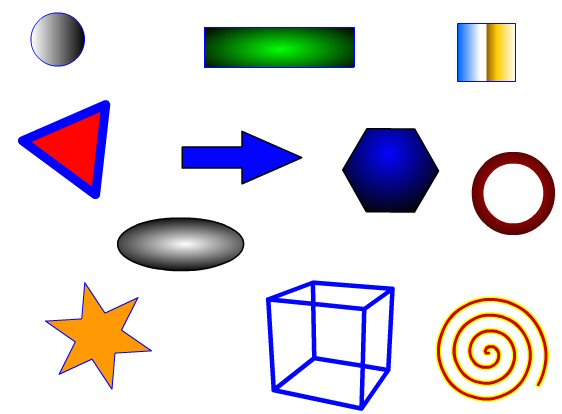
\includegraphics[width=11cm]{images/shapes.jpg}
  \caption[Przykłady różnych kształtów.]{Przykłady różnych
  kształtów~$^{\decimal{footnote}}$.}
  \label{shapes01}
\end{figure}
\footnotetext[\value{footnote}]{\url{http://www.parapal-online.co.uk/picture_dict/shapes.html}}


Dzięki zastosowaniu relacji przestrzennej między kształtami (przyleganie,
styczność, zawieranie, itp.), możliwe jest tworzenie innych bardziej złożonych
kształtów, np: opierając się na wiedzy na temat położenia dwóch figur, można
wykonać ich sumę, różnicę, lub inną operację, co daje większe zróżnicowanie
efektów. Dodatkowo, dobór produkcji do wykonania może być uwarunkowany
położeniem dwóch kształtów względem siebie.

%% rys str. 29

Do modyfikowania kształtów stosuje się proste operacje np.: przesunięcie,
rotacja, skalowanie i lustrzane odbicie względem prostej. Możliwe jest
zdefiniowanie większego zbioru operacji dodając nowe bądź poprzez połączenie już
istniejących transformacji w bardziej złożone.

\begin{figure}[h!]
  \centering
  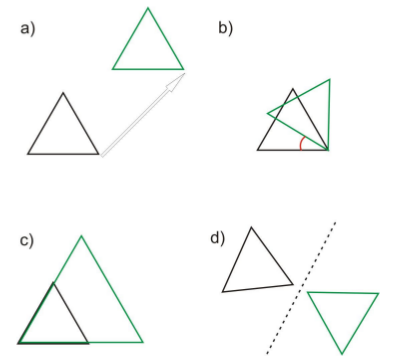
\includegraphics[width=8cm]{images/shapes02.png}
  \caption{Podstawowe transformacje w gramatykach kształtu a) przesunięcie, b)
  rotacja, c) skalowanie, d) lustrzane odbicie.\cite{gaudi}}
  \label{shapes02}
\end{figure}


Na ilustracji~\ref{etykietowanie} przedstawiony został przykład zastosowania
etykietowania kształtów. Etykieta determinuje tu sposób wykonania kolejnej produkcji. Dzięki
wprowadzeniu takiego rozwiązania można, za pomocą małego zbioru produkcji,
uzyskać bardziej złożone i zróżnicowane kształty. Możliwe jest wprowadzenie
kilku rodzajów etykietowania. Reguły mogą ponadto modyfikować istniejące
etykiety - zmienić ich położenie względem kształtu, usunąć etykietę, zastąpić
etykietę jednego rodzaju innym.

\begin{figure}[h!]
  \centering
  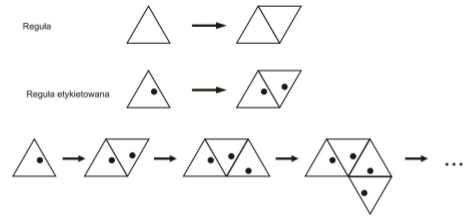
\includegraphics[width=12cm]{images/etykietowanie.png}
  \caption{Proces derywacji z zastosowaniem etykietowania.\cite{gaudi}}
  \label{etykietowanie}
\end{figure}

Gramatyki kształtu ze względu na swoje cechy stosowane są zazwyczaj do tworzenia
dwuwymiarowych obiektów, takich jak np.: posadzki, witraże, plany podstaw
budynków, ogrodów oraz plany zabudowy i plany pięter. Znajdują również
zastosowanie przy tworzeniu prostych, regularnych obiektów trójwymiarowych,
takich jak np. bryły budynków.

\subsection{Gramatyki --- podsumowanie.}
Ten rozdział miał na celu przedstawienie teorii dotyczącej gramatyk formalnych
skupiając się głównie na gramatykach stosowanych w grafice komputerowej.

W niniejszej pracy skupimy się na gramatykach kształtu oraz na gramatykach
grafowych (a raczej jej szczególnym rodzajem - gramatyki drzewiastej). Na
podstawie tych dwóch typów gramatyk spróbujemy opracować najwygodniejszą dla nas
gramatykę, za pomocą której postaramy się opisać głowę ludzką.

    \newpage
    \section{Jak ten problem rozwiązali inni?}
Nie ma zbyt wiele aplikacji podejmujących się próby generowania trójwymiarowych
głów na podstawie fotografii. Jedyne materiały jakie udało nam się znaleźć to
aplikacja FaceGen~\cite{link04} firmy Singular Inversions,
FaceShop~\cite{link05} firmy Abalone LLC oraz Facial Studio~\cite{facialstudio}
firmy itLocation. Wszystkie te aplikacje są niestety komercyjne i niewiele
jest informacji, na jakiej zasadzie generują one bryłę na podstawie zdjęć. Z
zebranej dokumentacji wynika, że zasada generacji polega na modyfikowaniu już
wcześniej przygotowanego modelu i takim modyfikacjom siatki, aby jak najbardziej
dopasować się do zdjęcia. Mimo, że proces generacji jest podobny w aplikacjach
to aplikacja FaceGen jest pod tym względem bardziej automatyczna. Nie trzeba
przekazywać aplikacji zbyt dużo punktów kontrolnych (miejsc gdzie znajduje się
oko, nos, usta itp.).

\addtocounter{footnote}{1}
\begin{figure}[h!]
  \centering
  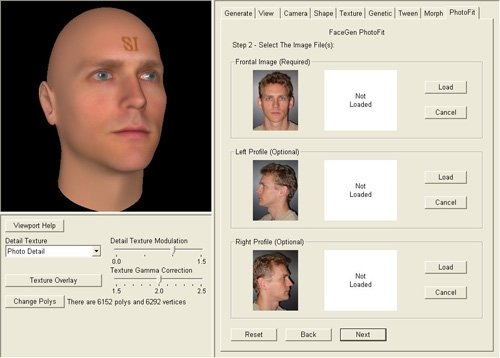
\includegraphics[width=9cm]{images/facegen.jpg}
  \caption[Singular Inversions FaceGen.]{Wygląd programu Singular Inversions
  FaceGen~$^{\decimal{footnote}}$.}
  \label{facegen}
\end{figure}
\footnotetext[\value{footnote}]{\url{http://www.facegen.com/}}
\addtocounter{footnote}{1}
\begin{figure}[h!]
  \centering
  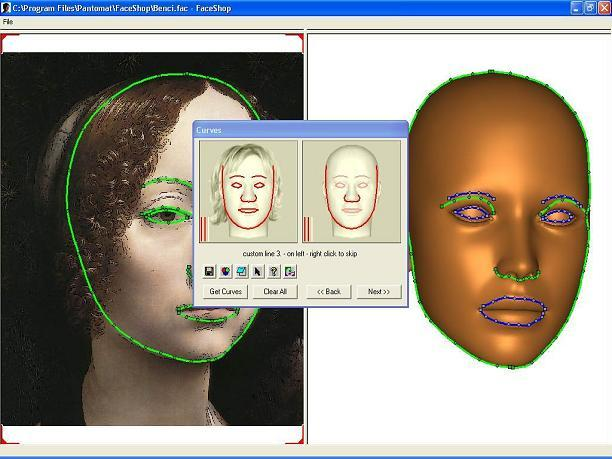
\includegraphics[width=9cm]{images/faceshop.jpg}
  \caption[Abalone LLC. FaceShop.]{Wygląd programu Abalone LLC.
  FaceShop~$^{\decimal{footnote}}$.}
  \label{faceshop}
\end{figure}
\footnotetext[\value{footnote}]{\url{http://downloads.zdnet.com/abstract.aspx?docid=780925}}
\addtocounter{footnote}{1}
\begin{figure}[h!]
  \centering
  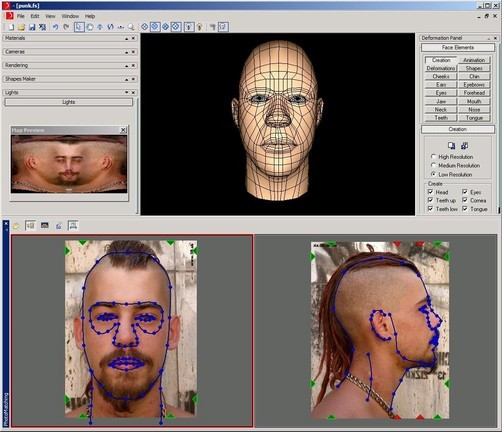
\includegraphics[width=9cm]{images/facialstudio.jpg}
  \caption[itLocation Facial Studio.]{Wygląd programu itLocation Facial
  Studio~$^{\decimal{footnote}}$.}
  \label{facialstudio}
\end{figure}
\footnotetext[\value{footnote}]{\url{http://www.youtube.com/watch?v=h4hfngdZH7Y}}

Wydawać by się mogło, że takie metody przenoszenia twarzy ludzkiej są
wystarczające. Problem pojawia się w przypadku, gdy analizowane zdjęcia nie są
odpowiedniej jakości np.: zawierają ujęcie częściowo zasłoniętej twarzy, zdjęcie
jest zniekształcone lub ma inne defekty. Wtedy bez ingerencji grafika
aplikacje dają oczekiwanych rezultatów.

Inną dość istotną wadą takiego podejścia jest np. wykorzystanie takiej
metodologii w kompresji obrazu opartej na syntezie obrazu do znanych wzorców.
Zakładając, że na scenie znajduje się 10 aktorów - synteza obrazu wygeneruje 10
siatek 3D (po jednej dla każdego aktora), więc tak naprawdę zysk na kompresji
nie będzie już tak duży.

\subsection{Skanowanie metodą wielu obrazów}
Tong-Yee Lee, Ping-Hsien Lin i Tz-Hsien Yang w swojej książce ''Photo-realistic
3D Head Modeling Using Multi-view Images,,~\cite{multiview} proponują dość
ciekawą koncepcje z wykorzystaniem stereowizualnej kamery. Obiekt jest
umieszczany na specjalnej podstawce~\ref{multiview} (nie jest ona konieczna ale
przy jej braku musimy pamiętać kolejność wykonywanych zdjęć), następnie wykonuje
się wiele zdjęć stereowizualnych dookoła obiektu. Na podstawie zdjęć
stereowizualnych na zasadzie stereometrii wyznacza się głębie obrazu (ang.
depth), a mając głębie obrazów dookoła obiektu możemy wolumetrycznie wyznaczyć
trójwymiarową bryłę. Jest to metoda interesująca, dość szybka, ale ma wady --
trzeba dysponować stereowizyjną kamerą oraz trzeba wykonywać zdjęcia dookoła
przedmiotów/osób.

\begin{figure}[h]
  \centering
  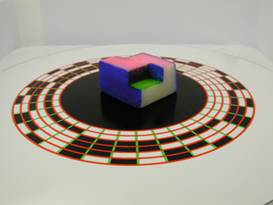
\includegraphics[width=9cm]{images/multi-view2.jpg}
  \caption{Przykładowy obiekt do skanowania metodą wielu
  obrazów~\cite{multiview}.}
  \label{multiview}
\end{figure}

Poniżej przedstawiamy dwa zdjęcia, jedno wykonane z lewego ``oka,, a drugie z
prawego, poniżej zaś wygenerowaną mapę głębokości na podstawie tych dwóch zdjęć.

\addtocounter{footnote}{1}
\begin{figure}[h!]
  \centering
  \subfloat{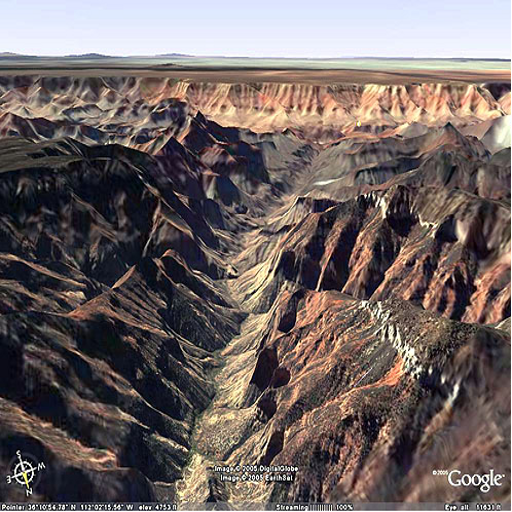
\includegraphics[width=5cm]{images/left.png}}
  \subfloat{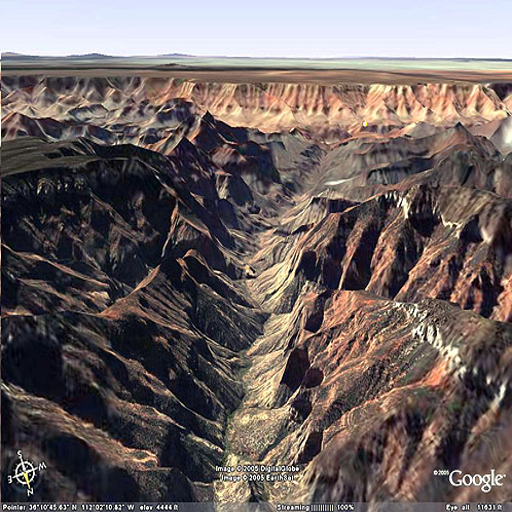
\includegraphics[width=5cm]{images/right.png}}
  \caption[Zdjęcia wykonane za pomocą stereowizyjnej
  kamery.]{Zdjęcia wykonane za pomocą stereowizyjnej
  kamery~$^{\decimal{footnote}}$.}
  \label{crosseye}
\end{figure}
\footnotetext[\value{footnote}]{\url{http://bbs.keyhole.com/ubb/ubbthreads.php?ubb=showflat&Number=58725}}

\begin{figure}[h!]
  \centering
  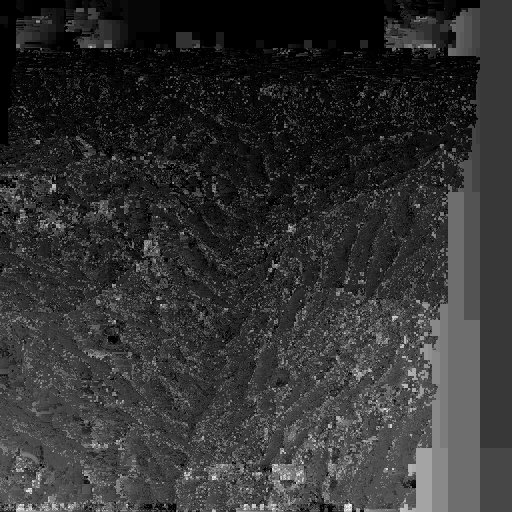
\includegraphics[width=5cm]{images/depth.png}
  \caption{Mapa głębi wyliczona na podstawie dwóch zdjęć wyżej (źródło własne).}
  \label{depth}
\end{figure}

Generowanie mapy głębokości na podstawie dwóch zdjęć jest dość proste, wystarczy
nakładać prawe zdjęcie na lewe przesuwając stopniowo prawe zdjęcie w lewo i
liczyć błąd (różnice pomiędzy obiema fotografiami). Minimalny błąd to jest
najlepsze dopasowanie. Zapamiętujemy przesunięcie jako wartość głębokości dla
całego obrazka. Następnie dzielimy obrazek na cztery części i wykonujemy to samo
dla każdej z tych części aż dojdziemy do pojedynczych pikseli. Poniżej znajduje
się kod takiego algorytmu napisany w C: funkcja {\em count\_err} licząca różnicę
pomiędzy fragmentami obrazu i funkcja {\em divide} przesuwająca prawy fragment
obrazu nad lewym i wyszukująca minimalny błąd, a następnie zapisująca
przesunięcie jako wartość głębokości i wykonująca to samo dla czterech
mniejszych części obrazu.

{
\small
\begin{lstlisting}[language=C++,numbers=left,frame=single,numberstyle=\tiny,backgroundcolor=\color{code_back},breaklines=true]
long count_err(int x, int y, int w, int h, int aw, int d)
{
  long err = 0;
  for (int j=y; j<y+h; j++)
  {
    int dy = j*aw;
    for (int i=x; i<x+w; i++)
    {
      int rx = i + d;
      if (rx > width || rx < 0) // continue if you came out beyond the image
        continue;

      char* rptr = (char*)&rdata[dy + rx]; // pointer to pixel on the right image
      char* lptr = (char*)&ldata[dy + i]; // pointer to pixel on the left image
      err += abs((*lptr++)-(*rptr++)); // color R
      err += abs((*lptr++)-(*rptr++)); // color G
      err += abs((*lptr++)-(*rptr++)); // color B
    }
  }
  return err;
}

void divide(int x, int y, int w, int h, int aw, int from, int to)
{
  long min = std::numeric_limits<long>::max();
  int move = 0;
  unsigned char d = depth[x+y*aw]; // current shift between images
  // find minimal error between two parts of images
  for (int m=from; m!=to; m++)
  {
    long err = count_err(x, y, w, h, aw, d+m);
    if (err < min)
    {
      min = err;
      move = m;
    }
  }

  // save new shift into depth
  unsigned char val = move + d > 0 ? (unsigned char)(move + d) : 0;
  for (int j=y; j<y+h; j++)
  {
    int dy = j*aw;
    for (int i=x; i<x+w; i++)
      depth[i+dy] = val;
  }

  // if image is too small to divide
  if (w < 2 && h < 2)
    return;

  // if error is still big
  if (min > 0)
  {
    // divide images to four smaller images
    int w2 = w >> 1;
    int h2 = h >> 1;
    int f = steps(w2);
    divide(x, y, w2, h2, aw, -(f>>1), f);
    divide(x+w2, y, w2, h2, aw, -(f>>1), f);
    divide(x, y+h2, w2, h2, aw, -(f>>1), f);
    divide(x+w2, y+h2, w2, h2, aw, -(f>>1), f);
  }
}
\end{lstlisting}
}

Dao Minh Lam, Ruizhi Z. Hong i Guilherme N. DeSouza w swojej książce
pod tytułem ,,3D human modeling using virtual multi-view stereopsis and
object-camera motion estimation''~\cite{multiview02} zaproponowali podobne
podejście z tą różnicą, że nie obraca się kamera tylko obiekt przed
kamerą (głównie żeby wyeliminować problem ciągłej kalibracji kamer) i na
podstawie porównywania obrazów jest wyznaczana pozycja wirtualnej kamery.
Poniżej przedstawione są efekty tego podejścia.

\begin{figure}[h!]
  \centering
  \subfloat{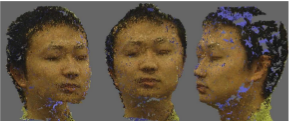
\includegraphics[width=7cm]{images/mv_02_01.png}}
  \qquad
  \subfloat{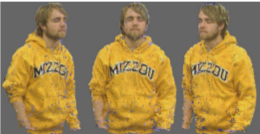
\includegraphics[width=7cm]{images/mv_02_02.png}}
  \caption{Rekonstrukcja obiektu z użyciem 70 zdjęć~\cite{multiview02}.}
  \label{mv_02_01}
\end{figure}

\begin{figure}[h!]
  \centering
  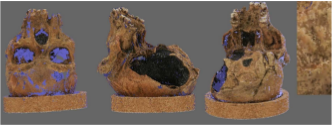
\includegraphics{images/mv_02_03.png}
  \caption{Rekonstrukcja czaszki~\cite{multiview02}.}
  \label{mv_02_02}
\end{figure}

\begin{figure}[h!]
  \centering
  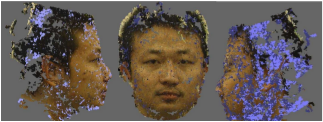
\includegraphics{images/mv_02_04.png}
  \caption{Rekonstrukcja twarzy z użyciem 16 zdjęć~\cite{multiview02}.}
  \label{mv_02_03}
\end{figure}

\subsection{Proceduralne modelowanie stworów}
Dość ciekawą koncepcję, powiązaną z niniejszą pracą, zaproponował Tomasz
Dąbrowski z Politechniki Gdańskiej w swojej pracy ,,Proceduralne modelowanie
stworów w Suboceanic''~\cite{dabrowski}. Opisana metoda polega na generowaniu
skomplikowanych zbiorów kul z niewielkiej liczby mniejszych zbiorów bazowych i
stochastycznych reguł podstawiania. Autor wykorzystał tu właśnie stochastyczne 
gramatyki kształtu, oparte na niewielu produkcjach, by wygenerować stwory.
Efekty jego pracy można zobaczyć na ilustracjach ~\ref{multiview} i
~\ref{multiview1}.

\begin{figure}[h!]
  \centering
  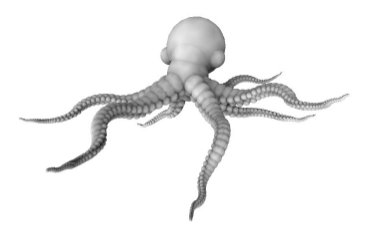
\includegraphics{images/suboceanic01.jpg}
  \caption{Model kulowy ośmiornicy, którą można spotkać nurkując w głębinach
  Suboceanic~\cite{dabrowski}.}
  \label{multiview}
\end{figure}

\begin{figure}[h!]
  \centering
  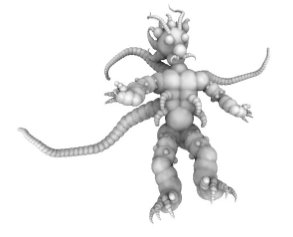
\includegraphics{images/suboceanic02.jpg}
  \caption{Proceduralny stworek zamieszkujący skaliste wybrzeża
  Suboceanic~\cite{dabrowski}.}
  \label{multiview1}
\end{figure}

Stwory opisane są za pomocą zbioru przetransformowanych i powielonych grup
bazowych, składających się ze zbioru kul, w którym każda kula zdefinowana jest
za pomocą środka w przestrzeni $\mathbb{R}^3$ i promienia. Każda grupa może
składać się z trzech typów kul:
\begin{enumerate}
  \item kule strukturalne, będące podstawą do wyznaczenia skóry stwora;
  \item kule atrapy, niewidoczne, pomocnicze kule w regułach podstawiania do
  wyznaczania dodatkowej translacji i skali podstawianej grupy;
  \item kule replikujące, do których przypisane są listy podstawień.
\end{enumerate}

\begin{figure}[h!]
  \centering
  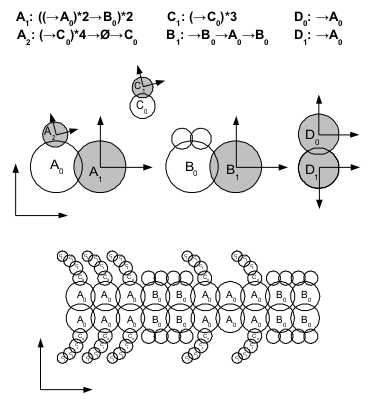
\includegraphics[width=12cm]{images/sys_podst.png}
  \caption{Przykładowy system podstawień składający się z 4 grup: A, B, C i
  D~\cite{dabrowski}.}
  \label{sys_podst}
\end{figure}

Element w liście podstawień to nic innego jak nieterminal i może on zawierać
szereg parametrów:
\begin{enumerate}
  \item symbol pusty: $\emptyset$, oznaczający brak podstawienia;
  \item indeks grupy kul i numer kuli w grupie, od której będzie realizowane
  podstawienie zadanej grupy zamiast kuli replikującej;
  \item opis transformacji podstawowej grupy (rotacja określona jako macierz
  lub kwaternion, symetryczne odbicie oraz skala określana jako stosunek
  promienia kuli replikującej do promienia kuli, od której rozpoczynamy
  podstawienie);
  \item zakres losowych odchyleń przy wyznaczaniu transformacji podstawowej
  grupy.
\end{enumerate}

W górnej części ilustracji~\ref{sys_podst} znajduje się definicja grup, reguł
transformacji i list podstawień. $A_1:((\longrightarrow A_0)*2\longrightarrow B_0)*2$ rozwija się do
$A_1:\longrightarrow A_0\longrightarrow A_0\longrightarrow
B_0\longrightarrow A_0\longrightarrow A_0\longrightarrow B_0$. Kule replikujące
to kule wypełnione kolorem. Na dole ilustracji znajduje się wynikowy zbiór kul
zaczynając od grupy D. Reguły umożliwiają swobodne łączenie różnych elementów ze
sobą i ich zwielokrotnianie.

Jak widać, autor wykorzystał gramatyki kształtu do modelowania stworów na
podobnej zasadzie jak to robi natura -- zakładając, że kule replikujące to
komórki macierzyste, a kule strukturalne to komórki skóry. Jak widać na
powyższych ilustracjach, koncepcja daje bardzo dobre rezultaty, a przy tym
wymaga niewielkiej ilości informacji o konstrukcji stwora (kilka reguł i zbiorów
kul). Zamierzeniem autorów tej pracy jest opracowanie gramatyki działającej na
podobnej zasadzie, która pozwoli na wygenerowanie ludzkiej głowy.

    \newpage
    \section{Przygotowanie gramatyki kształtu twarzy}
W tym rozdziale przedstawiony jest opis przeprowadzonej analizy struktury
głowy oraz dyskusja o tym, jak taką strukturę zamodelować przy użyciu
gramatyki kształtu.
Przed przystąpieniem do dalszej pracy, musiała zostać podjęta decyzja co
do poziomu szczegółowości wirtualnego odpowiednika głowy. Z założenia gramatyka
nie ma ograniczeń, więc nic nie stoi na przeszkodzie, aby zbudować model zawierający
wszystkie najbardziej elementarne części głowy. Jednak z uwagi na charakter
tej pracy oraz pożądany efekt docelowy zostaną pominięte wszystkie elementy
wewnętrzne. Najistotniejsze są części bezpośrednio tworzące zewnętrzną
strukturę. Warto jednak zaznaczyć, że jeżeli zaszłaby taka potrzeba to można
zamodelować wewnętrzną strukturę głowy i sterując parametrami obserwować wpływ
poszczególnych części na siebie. Wszystko zależy od złożoności gramatyki.
Na ilustracji~\ref{wiola_jpg} zaprezentowana jest przykładowa głowa
w różnych rzutach wraz z liniami na wybranych charakterystycznych poziomach.
Kolejne linie (od góry do dołu) oznaczają: czubek głowy, poziom górnej oraz
dolnej granicy oczu, koniec nosa, górną oraz dolną granicę warg i podbródek.

\begin{figure}[h!]
\centering
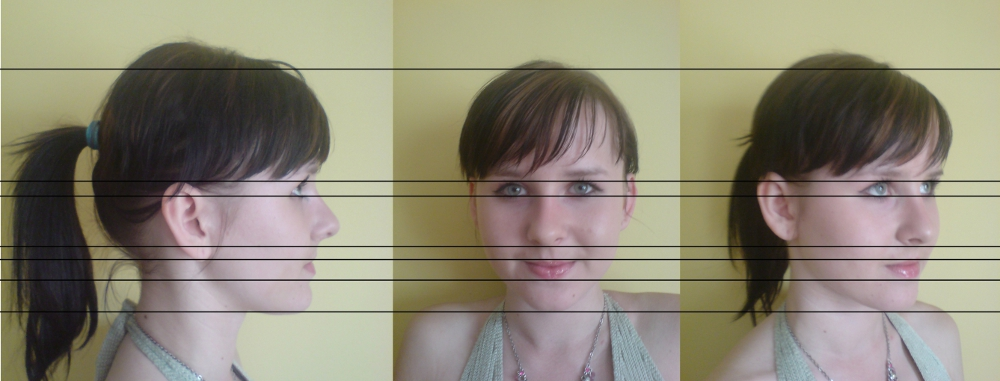
\includegraphics[width=14cm]{images/wiola.jpg}
\caption{Twarz w różnych rzutach wraz z liniami na charakterystycznych
poziomach (źródło własne).}
\label{wiola_jpg}
\end{figure}

Jak widać głowa składa się z:
\begin{itemize}
  \item uszu (para);
  \item oczu (para);
  \item nosa;
  \item ust;
  \item włosów;
  \item szyi;
  \item ogólnej struktury głowy, która nie należy do pozostałych części.
\end{itemize}
Jak można zauważyć, głowa jest symetryczna względem pionowej osi, co skłania ku
modelowaniu jednej części głowy, po czy zrobieniu jej lustrzanego odbicia. Można
jednak pójść inną drogą i modelować każdy element osobno. Oba sposoby mają plusy
i minusy, więc zdecydowano się zastosować rozwiązanie hybrydowe. Niektóre
obiekty, jak oczy, uszy, zostaną powielone natomiast ogólna struktura zostanie
utworzona jako całość.

\begin{figure}
\centering
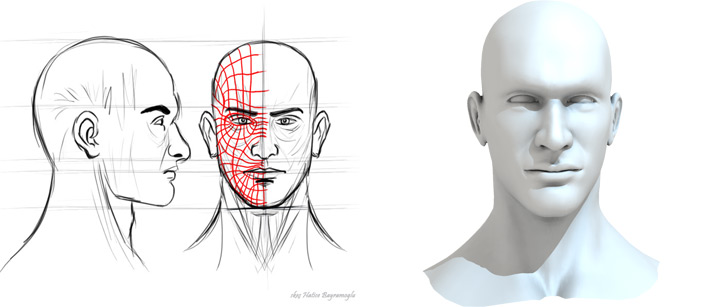
\includegraphics[width=12cm]{images/face-wire.jpg}
\caption{Szkic siatki głowy wraz z modyfikacją profilu~\cite{bayramoglu}}
\end{figure}

Można wyraźnie zauważyć trzy obszary: oko, nos z ustami, ucho. Mając już
oddzielone skomplikowane pod względem szczegółowości obszary, pozostała część
głowy nie jest skomplikowana i gładka więc można ją z powodzeniem zamodelować za
pomocą dosłownie kilku odpowiednio rozciągniętych sfer.

\subsection{Nieterminale w gramatyce kształtu}
Mając podzieloną strukturę głowy na mniejsze obszary należy zamodelować przy
użyciu podstawowych kształtów (łatwych do zapisania matematycznie) wszystkie
poszczególne obszary. Jako kształty łatwe do zapisania matematycznie
przyjęto: sferę, sześcian, płaszczyznę, cylinder, stożek i temu podobne. Za
pomocą tych kształtów oraz ich kombinacji (suma logiczna --- łączenie, różnica
--- wycinanie) można zamodelować dowolną część ludzkiej głowy. Jakość końcowa
wymodelowanej głowy zależy tylko od ilości wykorzystanych podstawowych
kształtów.

Wykorzystanie takich elementów nie będzie wystarczające do zbudowania modelu
więc zdecydowano się na dodanie trzech funkcji przekształcających obiekty:
przesunięcie, obrót i skalowanie. Nic nie stoi na przeszkodzie, żeby rozszerzyć
gramatykę o np. przekształcenia deformujące, takie jak: zwężenie, skręcenie i
wygięcie. Ograniczeniem jest tylko złożoność obliczeniowa danego
przekształcenia.

Kolejną sprawą jest łączenie podstawowych, przekształconych kształtów i do tego
celu wybraliśmy cztery podstawowe operacje Boolowskie: OR (suma logiczna), AND
(część wspólna), DIFF (różnica), XOR (różnica symetryczna). Te przekształcenia
umożliwią nam łączenie, wycinanie i tworzenie skomplikowanych obiektów z
wykorzystaniem dwóch podstawowych kształtów wspomnianych wyżej.

Do zamodelowania wspomnianych wcześniej symetrycznych części głowy należy dodać
funkcję MIRROR --- czyli odbicie lustrzane wymodelowanego już wcześniej
kształtu, względem wybranej płaszczyzny.

Wymienione wyżej podstawowe kształty i przekształcenia są wystarczające do
zamodelowania dowolnej głowy (a nawet całego ciała ludzkiego).

\subsection{Parser gramatyki kształtu}
Do tworzenia gramatyki kształtu zostanie wykorzystany tekstowy zapis kolejnych
operacji. Niezbędny jest również algorytm transformujący język zrozumiały dla
użytkownika programu do formy zrozumiałej przez program. Jako że celem tej pracy
nie jest opracowywanie parsera, zdecydowaliśmy się na wykorzystanie do tego celu
język LUA, ponieważ jest prosty do zaadoptowania do dowolnego projektu.
Korzystając dodatkowo z biblioteki tolua++ sprowadza się to do przygotowania
odpowiednio okomentowanych klas. Skrypt tolua++ parsuje plik nagłówkowy
opisujący klasę jaka ma być dostępna z poziomu skryptu LUA i zwraca plik
źródłowy, który wystarczy dołączyć do projektu.

\subsection{Reprezentacja gramatyki wewnątrz projektu}
Kolejnym ważnym krokiem do zbudowania projektu jest opracowanie struktury
przechowującej gramatykę, zachowując kolejność przetwarzania terminali i
nieterminali. Doskonałą do tego celu strukturą jest drzewo, gdzie liśćmi są
terminale, węzłami są nieterminale stanowiące operacje boolowskie, natomiast
przekształcenia takie jak rotacja, skalowanie i przesunięcie --- metodami
węzłów. Poniżej znajduje się fragment kodu ilustrujący omawianą reprezentację:

{
\small
\begin{lstlisting}[language=C++,numbers=left,frame=single,numberstyle=\tiny,backgroundcolor=\color{code_back},breaklines=true]
class Node
{
    protected:
        typedef boost::shared_ptr<Node> node_ptr;
        typedef const boost::shared_ptr<Node> const_node_ptr;
        typedef boost::weak_ptr<Node> parent_ptr;
        typedef const boost::weak_ptr<Node> const_parent_ptr;
        typedef std::list<node_ptr> t_child_list;

        const_node_ptr _this;
        parent_ptr parent;
        t_child_list childs;

    public:
        Node();
        virtual ~Node();

        bool has_parent();
        bool has_child();
		void attach(node_ptr new_child);
		void attach(node_ptr new_child, t_child_list::iterator it);
		void attach_to(node_ptr p);
		void attach_to(node_ptr p, t_child_list::iterator it);
		t_child_list::iterator detach();
		virtual node_ptr clone();
		virtual node_ptr clone(node_ptr n);
};
\end{lstlisting}
}

Klasa Node jest podstawowym elmentem drzewa, które jest tworzone z gramatyki.
Każdy węzeł może posiadać dowolną liczbę podelementów.

{
\small
\begin{lstlisting}[language=C++,numbers=left,frame=single,numberstyle=\tiny,backgroundcolor=\color{code_back},breaklines=true]
class Nonterminal // tolua_export
: public Node
{ // tolua_export
    protected:
        vl::mat4 tmpMatrix;
        vl::mat4 tmpMatrixInv;
        std::list<vl::mat4> modelMatrix;

    private:
        void buildModelMatrix();

    public:
        vl::mat4 getModelMatrix() const;

    public:
        // tolua_begin
        Nonterminal();
        virtual ~Nonterminal();

        void scale(float x, float y, float z);
        void translate(float x, float y, float z);
        void rotate(float p, float y, float r);
        // tolua_end

        void prepare();
        virtual bool hit(vl::vec4& p, vl::vec4& v, set& s);
        virtual bool hit(vl::vec4& p);
        virtual bool rayTrace(vl::vec4& p, vl::vec4& v, set& s);
        virtual bool rayTrace(vl::vec4& p);
        virtual Node::node_ptr clone();
        virtual Node::node_ptr clone(Node::node_ptr);
}; // tolua_export
\end{lstlisting}
}

Nonterminal jest klasą reprezentującą nieterminal gramatyki kształtu zmapowany
na element drzewa. Klasa pozwala na wykonanie kilku podstawowych transformacji
oraz udostępnia interfejs w postaci kilku metod, które muszą być
zaimplementowane, aby algorytm tworzenia kształtu przebiegał poprawnie:
\begin{itemize}
  \item Nonterminal::hit() -- ma za zadanie zwrócić wartość {\em true}, jeśli
  w wyznaczonym miejscu (określonym przez parametry) znajduje się obiekt. W
  przeciwnym razie metoda powinna zwrócić wartość {\em false}. Metoda ma dwie
  instancje --- z jednym parametrem oraz z trzema. Z jednym parametrem 
  (określającym położenie w przestrzeni $\mathbb{R}^3$) używana jest do
  generowania obiektu w przestrzeni wokselowej, gdyż mamy ustalony na stałe
  jej rozmiar i sprawdzamy woksel po wokselu czy znajduje się tam obiekt. Metoda z trzema parametrami jest
  wykorzystywana do renderowania metodą ray-tracingu (stąd 3 parametry: punkt
  wystrzelenia promienia, wektor promienia oraz zbiór trafień). Algorytm
  ray-tracingu będzie opisany dokładniej w dalszej części pracy;
  \item Nonterminal::rayTrace() -- metoda odpowiedzialna za kolejne etapy
  przeszukań przestrzeni. Podobnie jak w poprzednim przypadku
  posiada dwie instancje: jednoparametrową dla przeszukań w przestrzeni wokselowej i
  trzyparametrową dla przeszukań metodą ray-tracingu.
\end{itemize}

{
\small
\begin{lstlisting}[language=C++,numbers=left,frame=single,numberstyle=\tiny,backgroundcolor=\color{code_back},breaklines=true]
class Sphere : public Nonterminal { // tolua_export
    public:
    // tolua_begin
        Sphere();
        ~Sphere();
    //tolua_end
        virtual bool hit(vl::vec4& p, vl::vec4& v, set& s);
        virtual bool hit(vl::vec4& p);
        virtual Node::node_ptr clone();
}; // tolua_export

class Cylinder : public Nonterminal { // tolua_export
    public:
    // tolua_begin
        Cylinder();
        ~Cylinder();
    //tolua_end
        virtual bool hit(vl::vec4& p, vl::vec4& v, set& s);
        virtual bool hit(vl::vec4& p);
        virtual Node::node_ptr clone();
    private:
        float r;
        float h;
        vl::vec3 rdir;
        vl::vec3 hdir;
        vl::vec3 center;
}; // tolua_export

class And : public Nonterminal { // tolua_export
    public:
        And() {}
    // tolua_begin
        And(Nonterminal& t1, Nonterminal& t2);
        And(Nonterminal& t1, Nonterminal& t2, Nonterminal& t3);
        And(Nonterminal& t1, Nonterminal& t2, Nonterminal& t3, Nonterminal& t4);
        And(Nonterminal& t1, Nonterminal& t2, Nonterminal& t3, Nonterminal& t4, Nonterminal& t5);
        ~And();
    //tolua_end
        virtual bool rayTrace(vl::vec4& p, vl::vec4& v, set& s);
        virtual bool rayTrace(vl::vec4& p);
        virtual Node::node_ptr clone();
}; // tolua_export

class Or : public Nonterminal { // tolua_export
    public:
        Or() {}
    // tolua_begin
        Or(Nonterminal& t1, Nonterminal& t2);
        Or(Nonterminal& t1, Nonterminal& t2, Nonterminal& t3);
        Or(Nonterminal& t1, Nonterminal& t2, Nonterminal& t3, Nonterminal& t4);
        Or(Nonterminal& t1, Nonterminal& t2, Nonterminal& t3, Nonterminal& t4, Nonterminal& t5);
        ~Or();
    //tolua_end
        virtual bool rayTrace(vl::vec4& p, vl::vec4& v, set& s);
        virtual bool rayTrace(vl::vec4& p);
        virtual Node::node_ptr clone();
}; // tolua_export

class Diff : public Nonterminal { // tolua_export
    public:
        Diff() {}
    // tolua_begin
        Diff(Nonterminal& t1, Nonterminal& t2);
        Diff(Nonterminal& t1, Nonterminal& t2, Nonterminal& t3);
        Diff(Nonterminal& t1, Nonterminal& t2, Nonterminal& t3, Nonterminal& t4);
        Diff(Nonterminal& t1, Nonterminal& t2, Nonterminal& t3, Nonterminal& t4, Nonterminal& t5);
        ~Diff();
    //tolua_end
        virtual bool rayTrace(vl::vec4& p, vl::vec4& v, set& s);
        virtual bool rayTrace(vl::vec4& p);
        virtual Node::node_ptr clone();
}; // tolua_export

class Xor : public Nonterminal { // tolua_export
    public:
        Xor() {}
    // tolua_begin
        Xor(Nonterminal& f, Nonterminal& s);
        ~Xor();
    //tolua_end
        virtual bool rayTrace(vl::vec4& p, vl::vec4& v, set& s);
        virtual bool rayTrace(vl::vec4& p);
        virtual Node::node_ptr clone();
}; // tolua_export

class Mirror : public Nonterminal { // tolua_export
    public:
        Mirror() {}
    // tolua_begin
        Mirror(Nonterminal& t, char type);
        ~Mirror();
    //tolua_end
        virtual Node::node_ptr clone();
}; // tolua_export
\end{lstlisting}
}

Klasy Sphere oraz Cylinder to operatory tworzące kształty (ang.
brush\footnote{W terminologi grafiki komputerowej pojęcie to jest używane w
celu określenia obiektu o pewnym kształcie, który służy do tworzenia bądź
modyfikacji istniejącego modelu. Pędzle wykorzystywane są m.in. w programie
Sculptris, ZBrush do ,,rzeźbienia'' obiektów}.) odpowiednio sfery oraz cylindra.
Aby uzyskać odpowiedni rozmiar, pozycję oraz orientację należy wykorzystać
metory scale, transtale i rotate.
Na kształtach zdefiniowanych przez operatory Sphere i Cylinder można wykonywać
różne operacje logiczne oraz tworzyć lustrzane odbicia. Te funkcjonalności
zaimplementowane są przez klasy And, Or, Diff, Xor i Mirror.

    \newpage
    \section{Aplikacja}
Celem tego rozdziału jest opisanie praktycznych efektów pracy, czyli
aplikacji \emph{Facjator}, której przeznaczeniem jest umożliwienie tworzenia
gramatyki kształtu oraz przetworzenie tej gramatyki na trójwymiarowy model.

Aplikacja kliencka to samodzielny program dostępny w dwóch wersjach,
umożliwiających działanie na platformie Windows oraz Linux.

\subsection{Organizacja aplikacji}
Aplikacja została napisana w języku C++ przy wykorzystaniu środowiska
deweloperskiego Visual C++ 2008 (dla systemów Windows) oraz środowiska Code
Blocks (dla systemów z rodziny Linux). Projekt składa się z katalogu z plikami
źródłowymi oraz plikami projektu dla Visual C++ 2008. 
W projekcie wykorzystywanych jest kilka bibliotek zewnętrznych:
\begin{enumerate}
  \item Lua\footnote{\url{http://www.lua.org - język skryptowy}};
  \item toLua++\footnote{\url{http://www.codenix.com/~tolua/}};
  \item FLTK 1.1\footnote{\url{http://www.fltk.org/}};
  \item
  VisualizationLibrary\footnote{\url{http://www.visualizationlibrary.com/jetcms/}}.
\end{enumerate}
Lua jest to język skryptowy, który w bardzo prosty sposób można zintegrować z
natywnymi programami napisanymi w języku C++. Język charakteryzuje się wysoką
wydajnością oraz prostą składnią, dzięki czemu można w krótkim czasie opanować
składnię na tyle, aby pisać proste programy. Podstawowa znajomość składni jest
niezbędna dla projektanta gramatyki kształtu, ponieważ gramatyka w programie
jest definiowana w języku Lua. Razem z Lua wykorzystujemy w programie bibliotekę
pomocniczą toLua++, której zadaniem jest uproszczenie komunikacji pomiędzy
programem a wykonywanymi skryptami poprzez eksportowanie klas do Lua. Do
utworzenia interfejsu została wykorzystana biblioteka FLTK w wersji 1.1.
VisualizationLibrary to biblioteka, która upraszcza dodanie do aplikacji
funkcjonalności wyświetlania grafiki dwu i trójwymiarowej. Tworzy ona cienką
warstwę pośredniczącą pomiędzy programem a biblioteką OpenGL.

Kompilacja projektu jest zależna od systemu, na którym projekt jest budowany. Na
systemie Windows wymagane jest środowisko Visual C++ w wersji 2008, wersja
Express jest udostępniana za
darmo\footnote{\url{http://www.microsoft.com/visualstudio/en-us/products/2008-editions/express}}.
Kompilacja sprowadza się do wczytania projektu \emph{facjator.sln} i
uruchomieniu procesu budowania aplikacji (domyślnie skrót F7). W rezultacie
tworzony jest plik wykonywalny \emph{facjator.exe}.
W przypadku systemu Linux najwygodniejszą metodą kompilacji aplikacji jest
wczytanie projektu \emph{face.cbp} w środowisku
Code::Blocks\footnote{\url{http://www.codeblocks.org/}} również dostępnego za
darmo i rozpoczęcia procesu kompilacji wraz z budowaniem (skrót F9). Należy
również pamiętać, aby w systemie były dostępne wyżej wymienione biblioteki.

\subsection{Architektura aplikacji}
Proces generowania trójwymiarowego modelu składa się z kilku następujących po
sobie etapów:
\begin{enumerate}
  \item Utworzenie nowej gramatyki kształtu bądź wczytanie istniejącej gramatyki
  z pliku projektu zapisanego na dysku (wykonuje użytkownik);
  \item Utworzenie bądź aktualizacja parametrów w przypadku, gdy gramatyka
  zawiera parametry (wykonuje użytkownik);
  \item Parsowanie gramatyki kształtu i przetworzenie jej przy użyciu jednego z
  dwóch istniejących algorytmów (przetwarzanie w przestrzeni wokselowej lub
  raytracing);
  \item Utworzenie trójwymiarowej reprezentacji modelu i wyświetlenie jej w
  oknie programu.
\end{enumerate}
Zasady tworzenia gramatyki zostaną opisane w dalszej części pracy. W kolejnych
akapitach skupimy się na opisie algorytmów i mechanizmów wykorzystywanych przez
aplikację.
\subsubsection{Reprezentacja gramatyki jako modelu trójwymiarowego}
Przed przesłaniem obiektów trójwymiarowych do karty graficznej w celu ich
wyrenderowania, konieczne jest przetworzenie ich na listę trójkątów. Jednak
zanim to nastąpi, można wykorzystać dowolną metodę opisu struktury geometrii w
zależności od tego, która jest najbardziej przydatna w konkretnym zastosowaniu.
Wybór ostatecznie wykorzystywanej reprezentacji jest bardzo istotny ze względu na to, że determinuje sposób definiowania gramatyki oraz parametryzacji kształtu.
Wybór reprezentacji geometrii trójwymiarowej został ograniczony do trzech
znanych nam metod:
\begin{enumerate}
  \item Siatka trójkątów bądź czworoboków (zobacz ~\ref{fig:rep_geom1});
  \item Powierzchnie parametryczne (przy czym brano pod uwagę głównie
  hierarchiczne b-splajny, zobacz~\ref{fig:rep_geom2});
  \item Reprezentacja przy użyciu ograniczonej liczby dowolnych elementarnych
  obiektów, które mają swoją matematyczną reprezentację i przetwarzaniu takiej
  struktury w przestrzeni wokselowej lub przy użyciu algorytmu śledzenia
  promieni (ang. raytracing).
\end{enumerate}

{
\begin{figure}[h]
  \centering
  \subfloat[Siatka
  wielokątów.]{\label{fig:rep_geom1}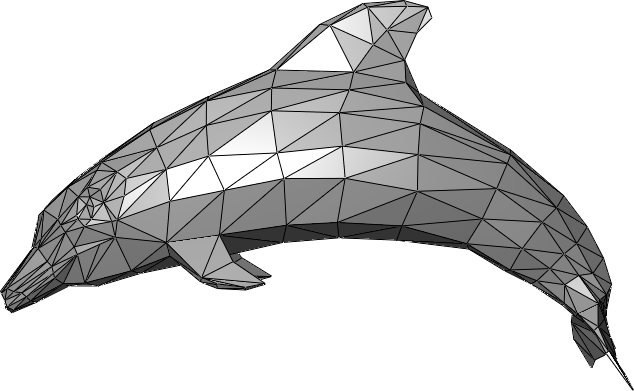
\includegraphics[width=6cm]{images/triangle_mesh.png}}
  \quad
  \subfloat[Hierarchiczne
  B-Splajny]{\label{fig:rep_geom2}\includegraphics[width=6cm]{images/hspline.jpg}}
  \quad
  \label{fig:rep_geom}
  \caption{Reprezentacje geometrii~$^{\decimal{footnote}}$.}
\end{figure}
\footnotetext[\value{footnote}]{\url{http://en.wikipedia.org/wiki/File:Dolphin_triangle_mesh.png},
\url{http://www.cgl.uwaterloo.ca/~ecdfourq/courses/cs779/project.html}}
}

Reprezentacja za pomocą siatki wielokątów\cite{link11}\cite{link12} jest
najprostszym ze sposobów reprezentacji modelu trójwymiarowego. Dodatkowo jest to
również format, w którym dane można przesyłać do karty graficznej, więc gdy
chcemy taką siatkę wyświetlić to z reguły nie jest wymagana żadna dodatkowa
konwersja. Siatka wielokątów~\ref{vef_image} w kontekście grafiki trójwymiarowej to
zbiór kilku elementów:
\begin{enumerate}
  \item wierzchołków, które są podstawowymi elementami definiującymi położenie
  punktów budujących model. Może być dowolnie wiele wierzchołków i same w sobie
  nie są wystarczające do tego, aby określić budowę modelu. Z wierzchołkami
  najczęściej powiązane są inne dane, takie jak --- kolor, współrzędne u,v dla
  tekstury nałożonej na siatkę oraz wektor normalny wykorzystywany do wyliczenia
  oświetlenia. Z perspektywy naszego programu dane te nie są istotne więc
  zostaną pominięte;
  \item krawędzi, które są zdefiniowane jako para dwóch wierzchołków, bez
  dodatkowych informacji;
  \item wielokątów (ang. face), które łączą krawędzie w grupy tworząc
  strukturę modelu. \emph{Face} może być dowolnym wielokątem, ale najczęściej
  wykorzystywanymi są trójkąt i czworokąt z uwagi na prostotę takiego rozwiązania.
\end{enumerate}
Mając definicję wielokątów można bez problemów określić powiązania pomiędzy
wierzchołkami i przygotować dane akceptowalne przez kartę graficzną.
Ten sposób reprezentacji geometrii ma dużą zaletę z uwagi na dosyć prostą
możliwość modyfikacji geometrii. Ponieważ wierzchołki definiują położenie 
punktów modelu, to w najprostszych przypadkach wystarczy modyfikować ich
położenie. Nieco większy stopień komplikacji mają algorytmy do operacji
logicznych na siatkach (and. constructive solid geometry\footnote{Technika
tworzenia skomplikowanych modeli polegająca na wykonywaniu operacji logicznych
na innych modelach.}), ale jest to możliwe do osiągnięcia. Niewątpliwie minusem
jest ograniczona szczegółowość odwzorowania modelowanych obiektów, które są
zależne od wielkości używanych wielokątów. Najprostszym
rozwiązaniem jest zwiększenie ich ilości przy równoczesnym zmniejszeniu ich
rozmiarów, jednakże szybko geometria ta staje się ciężka w zarządzaniu i wymaga
dużych zasobów obliczeniowych.
{
\begin{figure}[h]
  \centering
  \subfloat{\includegraphics[width=6cm]{images/Csg.png}}
  \label{csg_image}
  \caption{Operacje CSG na modelach pozwalają tworzyć skomplikowane
  kształty~$^{\decimal{footnote}}$.}
\end{figure}
\footnotetext[\value{footnote}]{\url{http://en.wikipedia.org/wiki/Constructive_solid_geometry}}
}
\begin{figure}
\centering
\includegraphics[width=8cm]{images/v_e_f.png}
\caption{Wierzchołki (a), krawędzie (b) oraz wielokąty (c) w modelu
trójwymiarowym (źródło własne).}
\label{vef_image}
\end{figure}

Główną wadą siatki wielokątów jest to, że przy jej użyciu ciężko modeluje się
gładkie powierzchnie. Do tego zadania o wiele lepiej nadaje się reprezentacja
geometrii za pomocą powierzchni parametrycznych. Rozwój prac nad powierzchniami
tego typu w grafice komputerowej zawdzięczamy w dużej mierze przemysłowi
motoryzacyjnemu, który potrzebował łatwego sposobu na tworzenie wizualizacji
samochodów i ich gładkich powierzchni.
W grafice często stosowane są powierzchnie
NURBS\footnote{http://en.wikipedia.org/wiki/Non-uniform\_rational\_B-spline}
(ang. Non-Uniform Rational B-Spline). Powierzchnia taka składa się z punktów kontrolnych, węzłów oraz wag punktów kontrolnych. Modyfikując te składowe parametry wpływa
się na wygląd powierzchni. Istotnym rozszerzeniem są powierzchnie typu
\emph{Hierarchical B-Spline} i możliwość dzielenia pojedynczego regionu zamiast
całej powierzchni. Daje to duże możliwości podczas modelowania obiektów, gdyż
pozwala na dodanie szczegółów tam, gdzie są niezbędne bez modyfikacji pozostałej
geometrii.
{
\begin{figure}[h]
  \centering
  \subfloat{\includegraphics[width=5cm]{images/worstG.jpg}}
  \quad
  \subfloat{\includegraphics[width=5cm]{images/worstL.jpg}}
  \quad
  \label{fig:hbspline}
  \caption{Zmodyfikowana powierzchnia parametryczna z
  lokalnymi podziałami~$^{\decimal{footnote}}$.}
\end{figure}
\footnotetext[\value{footnote}]{\url{http://www.cs.ubc.ca/nest/imager/contributions/forsey/dragon/hbsplines.html}}
}

Reprezentacja wokselowa wyróżnia inne podejście do problemu tworzenia i
przechowywania w pamięci modelu trójwymiarowego. Zaprezentowane wcześniej
sposoby reprezentacji geometrii skupiały się na tworzeniu samej zewnętrznej
powłoki modelu, natomiast woksele zajmują również wewnętrzną przestrzeń modelu.
Przy wykorzystaniu tej techniki, od razu można zauważyć podatność na
zastosowanie różnego rodzaju algorytmów logicznych na wokselach, głównie ze względu na
prostotę implementacji w porównaniu do wcześniej opisanych reprezentacji
geometrii, zwłaszcza powierzchni parametrycznych. Podstawowym elementem w tej
reprezentacji jest woksel. Jest to obiekt w przestrzeni trójwymiarowej
reprezentujący wartość. Przestrzeń przechowująca woksele ma postać tablicy
trójwymiarowej, gdzie na pojedynczy element tablicy przypada jeden woksel. Dane przechowywane przez woksele mogą być dowolnej
postaci i zależą od zastosowania. W najprostszym przypadku może to być
pojedyncza flaga, oznaczająca czy dany woksel jest zajęty (renderowalny) czy
nie (przeźroczysty). Tworzenie kształtów polega w takim przypadku na włączaniu i
wyłączaniu odpowiednich wokseli. W związku z tym, że dane sa przechowywane w
formie dyskretnej, może pojawić się aliasing\footnote{W grafice komputerowej
jest to zjawisko polegające na zniekształceniu obrazu w wyniku zbyt małej częstości
próbkowania, objawia się widocznymi \emph{schodkami} w miejscu, gdzie powinny
był gładkie kształty.}. Częściowo można rozwiązać ten problem poprzez
zwiększenie liczby wokseli, jednak pociąga to za sobą zwiększone zapotrzebowanie
na zasoby obliczeniowe komputera. Do usunięcia aliasingu może się również
przyczynić algorytm użyty do renderowania obiektów wokselowych np. marching
cubes.

{
\begin{figure}[h]
  \centering
  \subfloat{\includegraphics[width=5cm]{images/voxel_sphere.jpg}}
  \label{fig:voxel_sphere}
  \caption{Sfera wyświetlona jako obiekt wokselowy~$^{\decimal{footnote}}$.}
\end{figure}
\footnotetext[\value{footnote}]{\url{http://www.plotz.co.uk}}
}

\subsubsection{Parametryzacja geometrii}
Jednym z problemów związanych z geometryczną reprezentacją głowy jest
parametryzacja geometrii. Każdy z opisanych wcześniej sposobów reprezentacji
przy użyciu wielokątów najbardziej odpowiednie wydaje się
parametryzowanie położenia poszczególnych wierzchołków budujących strukturę
modelu. Możliwości wydają się nieograniczone, jednak dość łatwo można sobie
wyobrazić trudność polegającą na zachowaniu dobrego efektu wizualnego przy
próbie symulowania gładkich powierzchni. Rozwiązaniem może być zastosowanie
modyfikatorów proporcjonalnych (znanych z różnych programów służących do edycji
trójwymiarowych modeli), które są wykorzystywane do zachowania gładkości
modyfikowanej powierzchni. Z naszych prób wynika, że efekt może nie być
zadowalający przy dużym skomplikowaniu modelu. Biorąc pod uwagę modyfikatory proporcjonalne, dosyć trudne wydaje się wyizolowanie modyfikowanych wierzchołków, w sytuacji gdy blisko siebie znajdują się różne, niezależne powierzchnie. W przypadku powierzchni parametrycznych najlepszym sposobem parametryzacji jest
modyfikowanie punktów kontrolnych powierzchni. Powierzchnie tego typu zachowują swoją gładkość w przypadku zmiany parametrów,
co wydaje się być dużym plusem, biorąc pod uwagę charakter tworzonego przez nas
modelu. Można powiedzieć, że modyfikowane powierzchnie zachowywałyby
naturalność.

Tak jak w reprezentacji siatki do budowania modelu używa się wielokątów,
w reprezentacji parametrycznej hierachicznych b-splajnów, tak w reprezentacji
wokselowej podstawowym elementem jest pojedynczy woksel. Rozsądne wydaje się
przejście na wyższy poziom i budowanie modeli wykorzystując podstawowe
elementy, jak sfery, sześciany itp.. W kontekście parametryzacji oznacza,
że można poddawać modyfikacji parametry tych obiektów np. pozycję,
obrót, skalę. Przedstawione dotąd sposoby parametryzacji dotyczyły pojedynczych
elementów reprezentacji geometrycznych. Wydaje się jednak, że niezbędne jest również parametryzowanie w kontekście kilku elementów np. wykonywanie operacji logicznych. W każdej
reprezentacji jest to możliwe, jednak poziom komplikacji jest bardzo różny.
Biorąc pod uwagę nasze potrzeby zdecydowano, że zostanie wykorzystana
reprezentacja wokselowa. Duże znaczenie przy wyborze miała w miarę
bezproblemowa implementacja kilku operacji, którą później planowaliśmy
wykorzystać w tworzeniu i parametryzacji modelu.

\subsubsection{Przetwarzanie gramatyki w przestrzeni wokselowej}
Przetwarzanie gramatyki kształtu w przestrzeni wokselowej sprowadza się
do wykonania operacji tworzących drzewo gramatyki (ilustracja
~\ref{tree_traversal_algo}) na każdym wokselu. Każdy woksel ma unikalną
współrzędną, która wykorzystywana jest do sprawdzania poprawności w kontekście
wszystkich terminali i nieterminali.

\subsubsection{Ray-tracing}
Model matematycznego przechowywania geometrii zastosowany w pracy wpłynął na
zastosowanie w programie alternatywnego algorytmu renderowania:
ray-tracingu\footnote{\url{http://en.wikipedia.org/wiki/Ray\_tracing\_\%28graphics\%29}}.
O samej metodzie renderowania metodą ray-tracingu można znaleźć wiele materiałów
w sieci dlatego poniżej opisana zostanie jedynie implementacja w programie
\emph{Facjator}.

Mając reprezentacje matematyczną obiektów (pomijając fakturę obiektów), idea nie
różni się od klasycznej metody ray-tracingu -- najpierw wypuszczany jest promień
z pozycji kamery, kierowany jest do konkretnego piksela na płaszczyźnie
rzutowania i dalej rzutowany w przestrzeń. Następnie badane są przecięcia z
obiektami znajdującymi się na scenie. Jeżeli nastąpiła kolizja to wyliczamy
natężenie światła w punkcie trafienia na podstawie wektora normalnego do
powierzchni, wektora do kamery i wektora do światła; jeśli nie było trafienia,
ustawiany jest kolor czarny i cały proces jest powtarzany dla kolejnego piksela.
Istnieje tylko jedna sytuacja, w której klasyczna metoda zawiedzie,
zaprezentowana jest na ilustracji~\ref{ray_trace01}

\begin{figure}[h]
  \centering
  \includegraphics[width=12cm]{images/ray_trace01.png}
  \caption{Problem ray-tracingu i operacji boolowskich (źródło własne).}
  \label{ray_trace01}
\end{figure}

W przypadku klasycznego renderingu, informacja o drugim obiekcie jest tracona,
gdyż jest renderowany obiekt, który jest bliżej kamery (pierwsza kula
zakrywa drugą kulę, więc zostanie wyrenderowana tylko pierwsza kula).
Zakładając, że pierwsza kula zostaje wycięta ze sceny operacją {\em Diff} to
brak informacji o dalszym obiekcie spowoduje, że nie zostanie wyrenderowany
żaden obiekt (a powinien być drugi).

Aby rozwiązać ten problem została zaimplementowana taka metoda, która pozwoli
zapamiętać wszystkie obiekty na drodze promienia. W tym celu opracowano klasę
{\em set} reprezentującą zbiór odcinków, gdzie jeden odcinek reprezentuje obszar
wewnątrz obiektu (ilustracja~\ref{ray_trace02}).

\begin{figure}[h]
  \centering
  \includegraphics[width=12cm]{images/ray_trace02.png}
  \caption{Przykład zastosowania klasy {\em set} (źródło własne).}
  \label{ray_trace02}
\end{figure}
Dzięki użyciu klasy {\em set} operacje boolowskie sprowadzają się do operacji na
zbiorach odcinków (suma odcinków, różnica odcinków, część wspólna odcinków
itp.). Po wykonaniu wszystkich operacji na obiektach, wyciągany jest ze zbioru
element położony najbliżej kamery (minimum ze zbioru). Obiekt ten zostaje
wyrenderowany.

\begin{figure}[h]
  \centering
  \includegraphics[width=12cm]{images/tree_traversal.PNG}
  \caption{Implementacja przetwarzania drzewa gramatyki kształtu (źródło
  własne).}
  \label{tree_traversal_algo}
\end{figure}

\subsubsection{Interfejs aplikacji}
Główne okno aplikacji składa się z kilku podokien o różnym przeznaczeniu.
Zgodnie z oznaczeniami na ilustracji~\ref{main_window} poszczególne elementy
okna to:
\begin{enumerate}
  \item menu aplikacji,
  \begin{enumerate}
    \item File-New - utworzenie nowego, pustego projektu;
    \item File-Open - okno wyboru pliku projektu do wczytania, istniejące
    parametry oraz skrypt gramatyki zostaną zastąpione;
    \item File-Save - zapisanie zmian w projekcie do aktywnego pliku na dysku;
    \item File-Save As - zapisanie aktualnego projektu do nowego pliku;
    \item Edit-Undo - cofnięcie ostatniej operacji edycji;
    \item Edit-Redo - ponowienie ostatniej operacji edycji;
    \item Edit-Cut - wycięcie zaznaczonego tekstu;
    \item Edit-Copy - kopiowanie zaznaczonego tekstu;
    \item Edit-Paste - wklejenie skopiowanego wcześniej tekstu;
  \end{enumerate}
  \item okno wyświetlające efekt końcowy przetwarzania gramatyki czyli gotowy
  model trójwymiarowy. Aby uaktywnić opcję orbitowania kamery wokół modelu
  należy kliknąć i przytrzymać prawy przycisk myszy w oknie oraz poruszać
  kursorem, zwolnienie przycisku wyłączy funkcję orbitowania (opcja dostępna
  tylko podczas przetwarzania gramatyki w przestrzeni wokselowej);
  \item okna pozwalające na wczytanie wzorcowych obrazów tworzonego modelu.
  Wciśnięcie prawego przycisku myszy wyświetla menu podręczne,
  \item edytor skryptu gramatyki;
  \item przyciski do wykonywania operacji:
  \begin{enumerate}
    \item przetwarzanie gramatyki w przestrzeni wokselowej (Compile);
    \item przetwarzanie gramatyki algorytmem śledzenia promieni (Ray trace);
    \item pole tekstowe do wprowadzania rozmiaru przestrzeni wokselowej oraz do
    aktualizacji tej wartości w projekcie (Update size);
    \item przycisk do przywracania domyślnych ustawień kamery (Reset camera);
    \item przyciski do ustawiania kamery z wybranej strony elementu: lewej
    (\emph{Left}), prawej (\emph{Right}), z góry (\emph{Top}), od dołu
    (\emph{Bottom}), od przodu (\emph{Front}), od tyłu (\emph{Back}).
  \end{enumerate}
  \item okno z listą zdefiniowanych parametrów oraz przyciskami umożliwiającymi
  dodawanie nowych, usuwanie, edycję istniejących parametrów.
\end{enumerate}

\begin{figure}[h]
  \centering
  \includegraphics[width=0.7\textwidth]{images/ui.jpg}
  \caption{Główne okno aplikacji (źródło własne)}
  \label{main_window}
\end{figure}

\begin{figure}[h]
  \centering
  \subfloat{\includegraphics[width=5cm]{images/ui_def_param.jpg}}
  \caption{Okno definicji nowego parametru (źródło własne)}
  \label{new_param_window}
  \quad
  \subfloat{\includegraphics[width=5cm]{images/ui_edit_param.jpg}}
  \caption{Okno edycji istniejącego parametru (źródło własne)}
  \label{edit_param_window}
\end{figure}
Wybranie przycisku dodawania nowego parametru otwiera okno zaprezentowane na
ilustracji~\ref{new_param_window}. Można w nim wprowadzić unikalną nazwę
parametru opisującą jego funkcję, typ danych przechowywanych przez parametr oraz domyślną
wartość parametru. Zdefiniowane parametry można edytować zaznaczając je na
liście i wybierając przycisk edycji. Okno edycji przedstawione na
ilustracji~\ref{edit_param_window} pozwala na zmianę nazwy oraz wartości
parametru. Po utworzeniu parametru nie ma możliwości zmiany typu przechowywanych danych.
Z poziomu gramatyki kształtu do parametru odwołujemy się przy użyciu jego nazwy.

\subsubsection{Operacje oraz modyfikatory w gramatyce kształtu}
W zaimplementowanym programie zostało wykorzystanych kilka elementarnych obiektów oraz
modyfikatorów bazujących na technikach \emph{CSG}\footnote{ang. Constructive
Solid Geometry}. W tabelach~\ref{elements_table}, \ref{transforms_table},
\ref{operations_table}, \ref{misc_table} zostały przedstawione wszystkie
możliwości oraz przykłady wykorzystania modyfikatorów.

\setlength\fboxsep{2pt}
\setlength\fboxrule{0pt}
{
\noindent
\begin{center}
\begin{table}[hb]
\begin{tabular}{| p{0.55\textwidth} | p{0.35\textwidth} | }
  \hline
  \rowcolor{lightgray} Opis obiektu & Przykład użycia \\ \hline \hline
  
  \textbf{Sześcian}\newline
  Generuje model sześcianu o rozmiarach 2x2x2 &
  local cube = Cube(); \newline draw(cube); \\ \hline
  \multicolumn{2}{|c|}{\fbox{\includegraphics[width=4cm]{images/elem_cube.jpg}}}
  \\
  \hline
  
  \textbf{Sfera}\newline
  Generuje model sfery o promieniu równym 1 &
  local sphere = Sphere(); \newline draw(sphere); \\ \hline
  \multicolumn{2}{|c|}{\fbox{\includegraphics[width=4cm]{images/elem_sphere.jpg}}}
  \\
  \hline
\end{tabular}
\caption{Podstawowe modele (obiekty elementarne) dostępne w gramatyce kształtu
(źródło własne)}
\label{elements_table}
\end{table}
\end{center}
}

{
\noindent
\begin{center}
\begin{table}[hp]
\begin{tabular}{| p{0.55\textwidth} | p{0.35\textwidth} | }
  \hline
  \rowcolor{lightgray} Opis obiektu & Przykład użycia \\ \hline \hline  
  \textbf{Walec}
  \newline Generuje model walca kołowego prostego o promieniu podstawy równym 1
  oraz wysokości równej 2 &
  local cylinder = Cylinder(); \newline draw(cylinder); \\ \hline
  \multicolumn{2}{|c|}{\fbox{\includegraphics[width=4cm]{images/elem_cylinder.jpg}}}
  \\
  \hline
  
  \textbf{Stożek}
  \newline Generuje model stożka prostego o promieniu podstawy równym 1 oraz
  wysokości równej 1 & local cone = Cone(); \newline draw(cone); \\
  \hline
  \multicolumn{2}{|c|}{\fbox{\includegraphics[width=4cm]{images/elem_cone.jpg}}}
  \\
  \hline

  \textbf{Torus}
  \newline Generuje torus o podanych promieniach. Pierwszy argument to promień
  torusa, drugi to promień okręgu tworzącego tunel & local torus = Torus(0.66,
  0.23); \newline draw(torus); \\ \hline
  \multicolumn{2}{|c|}{\includegraphics[width=4cm]{images/elem_torus.jpg}}
  \\
  \hline
\end{tabular}
\caption{Podstawowe modele (obiekty elementarne) dostępne w gramatyce kształtu
cd.}
\label{elements_table}
\end{table}
\end{center}
}

{
\noindent
\begin{center}
\begin{table}[hp]
\begin{tabular}{| p{0.55\textwidth} | p{0.35\textwidth} | }
  \hline
  \rowcolor{lightgray} Opis transformacji & Przykład użycia \\ \hline \hline
  
  \textbf{Translacja}\newline
  Przesuwa obiekt, na rzecz którego następuje wywołanie o wybrany wektor &
  local cube = Cube(); \newline cube:translate(0.5, 0, 0) \newline --
  przesunięcie o 0.5 jednostek wzdłuż osi X \\ \hline
  \multicolumn{2}{|c|}{\fbox{\includegraphics[width=8cm]{images/op_translate.jpg}}}
  \\
  \hline
  
  \textbf{Rotacja}\newline
  Obraca obiekt, na rzecz którego następuje wywołanie o kąt wokół osi X, Y i Z.
  Wartość kąta jest podawana w radianach (rotate) bądź stopniach (rotateDeg) &
  local cube = Cube(); \newline cube:rotateDeg(0.0, 0, 30.0) \newline --
  obrót o 30 stopni wokół osi Z \\ \hline
  \multicolumn{2}{|c|}{\fbox{\includegraphics[width=8cm]{images/op_rotate.jpg}}}
  \\
  \hline
  
  \textbf{Skalowanie}
  Skaluje obiekt, na rzecz którego następuje wywołanie o podaną wartość wzdłuż
  osi X, Y, Z &
  local cube = Cube(); \newline cube:scale(1, 0.5, 1) \newline
  -- skaluje obiekt do połowy jego oryginalnego wymiaru wzdłuż osi Y; \\ \hline
  \multicolumn{2}{|c|}{\fbox{\includegraphics[width=8cm]{images/op_scale.jpg}}}
  \\
  \hline
\end{tabular}
\caption{Transformacje na obiektach elementarnych (zobacz~\ref{elements_table})
dostępne w gramatyce kształtu (źródło własne)}
\label{transforms_table}
\end{table}
\end{center}
}

{
\noindent
\begin{center}
\begin{table}[hp]
\begin{tabular}{| p{0.40\textwidth} | p{0.50\textwidth} | }
  \hline
  \rowcolor{lightgray} Typ operacji & Przykład użycia \\ \hline \hline
  
  \textbf{Suma elememtów} &
  local op = Or(sphere, cylinder); \newline draw(op); \\ \hline
  \multicolumn{2}{|c|}{\fbox{\includegraphics[height=4cm]{images/logic_or.jpg}}}
  \\
  \hline
  
  \textbf{Część wspólna} &
  local op = And(sphere, cylinder); \newline draw(op); \\ \hline
  \multicolumn{2}{|c|}{\fbox{\includegraphics[height=4cm]{images/logic_and.jpg}}}
  \\
  \hline
  
  \textbf{Różnica} &
  local op = Diff(sphere, cylinder); \newline draw(op); \\ \hline
  \multicolumn{2}{|c|}{\fbox{\includegraphics[height=4cm]{images/logic_diff.jpg}}}
  \\
  \hline
  
  \textbf{Różnica symetryczna}, w przykładzie przekrój modelu po wykonanej
  operacji Xor &
  local op = Xor(sphere, cylinder); \newline draw(op); \\ \hline
  \multicolumn{2}{|c|}{\fbox{\includegraphics[height=4cm]{images/logic_xor.jpg}}}
  \\
  \hline
\end{tabular}
\caption{Operacje logiczne na obiektach elementarnych
(zobacz~\ref{elements_table}) dostępne z poziomu gramatyki kształtu (źródło
własne)}
\label{operations_table}
\end{table}
\end{center}
}

{
\noindent
\begin{center}
\begin{table}[hp]
\begin{tabular}{| p{0.50\textwidth} | p{0.4\textwidth} | }
  \hline
  \rowcolor{lightgray} Opis obiektu & Przykład użycia \\ \hline \hline
  
  \textbf{Odbicie lustrzane}\newline
  Generuje kopię elementu odbitą względem osi X, Y lub Z. Drugi parametr w
  konstruktorze obiektu Mirror oznacza oś odbicia przyjmując, że 0 - oś X, 1 -
  oś Y, 2 - oś Z &
  local elem = Cube(); \newline elem scale(0.3, 0.3, 0.3); \newline
  elem translate(-1.2, 0, 0); \newline local mirror = Mirror(elem, 0); \newline
  local both = Or(elem, mirror); \newline draw(both); \\ \hline
  \multicolumn{2}{|c|}{\fbox{\includegraphics[height=4cm]{images/misc_mirror.jpg}}}
  \\
  \hline

  \textbf{Płaszczyzna}
  \newline Tworzy płaszczyznę, której normalna jest wektorem (1, 0, 0). &
  local cylinder = Cylinder(); \newline cylinder:scale(0.6, 0.6, 0.6); \newline
  local plane = Plane(); \newline plane:rotateDeg(0, -15, 0); \newline local op
  = And(cylinder, plane); \newline draw(op); \\ \hline
  \multicolumn{2}{|c|}{\fbox{\includegraphics[height=4cm]{images/misc_plane.jpg}}}
  \\
  \hline
  
  \textbf{Dostęp do parametrów}
  \newline Aby w skrypcie gramatyki uzyskać dostęp do parametrów
  zdefiniowanych w programie należy skorzystać z metod klasy \emph{params}
  podając nazwę parametru. &
  local floatParam = params:getParamFloat(``Nazwa''); \newline local intParam
  = params:getParamInt(``Nazwa 1''); \newline local stringParam =
  params:getParamString(``Nazwa 2'');
  \\
  \hline
\end{tabular}
\caption{Dodatkowe operacje i modyfikatory (źródło własne)}
\label{misc_table}
\end{table}
\end{center}
}

{
\noindent
\begin{center}
\begin{table}[!htbp]
\begin{tabular}{| p{0.50\textwidth} | p{0.4\textwidth} | }
  \hline
  \rowcolor{lightgray} Opis obiektu & Przykład użycia \\ \hline \hline
  
  \textbf{Modyfikator płaszczyzny}
  \newline Tworzy płaszczyznę ,,odpychającą'' woksele. Domyślna normalna
  powierzchni jest wektorem (1, 0, 0). Jako parametr konstruktora należy podać
  modyfikowany obiekt gramatyki, zasięg działania modyfikatora oraz
  siłę odpychania (maleje wraz ze wzrostem odległości punktu od powierzchni). Do
  modyfikowania położenia, orientacji i skali powierzchni należy używać metod z
  przedrostkiem \emph{p\_} np. \emph{p\_rotateDeg(10, 0, 0)}. & local sphere =
  Sphere(); \newline local mod = PlaneProp(sphere, 1, 0.5); \newline mod:p\_rotateDeg(0, 180, 0); \newline mod:p\_translate(1, 0, 0); \newline draw(mod); \\ \hline
  \multicolumn{2}{|c|}{\fbox{\includegraphics[height=4cm]{images/op_push.jpg}}}
  \\
  \hline
\end{tabular}
\caption{Dodatkowe operacje i modyfikatory cd. (źródło własne)}
\label{misc_table1}
\end{table}
\end{center}
}

    \newpage
    \section{Symulacje i testy}
W tym rozdziale przedstawione zostaną gramatyki renderujące różne
przedmioty oraz metody ich tworzenia. W kolejnych podrozdziałach zostaną one
dokładnie opisane. Po zaznajomieniu się z metodologią tworzenia gramatyk
zaprezentowane zostaną poszczególne elementy głowy, następnie połączone zostaną
w jedną całość.

\subsection{Proste obiekty}
Do przetestowania gramatyk kształtów wybraliśmy dwa obiekty, które mają
dosyć prostą strukturę ale jednocześnie pozwalają na wykorzystanie większości
dostępnych możliwości programu..
\subsubsection{Kostka do gry}
Pierwszym elementem poddanym analizie jest kostka do gry. Jest to element dość
prosty do zamodelowania, ponieważ można go wykonać z jednego sześcianu (ang.
cube) i 21 kul, którymi zostaną wycięte otwory oznaczające ilość oczek na
konkretnej ściance kostki. Aby zadanie nieco utrudnić, dodana zostanie możliwość
wygładzania krawędzi kostki, oraz dwa parametry określające stopień wygładzenia
krawędzi i wielkość kostki.

Poniżej znajduje się kod tworzący kostkę oraz wygenerowana za pomocą aplikacji
kostka:
\begin{figure}[h!]
  \centering
  \subfloat[border = 0.1, size = 0.8]{\includegraphics[width=0.4\textwidth]{images/tests/kostka01.png}}
  \qquad
  \subfloat[border = 0.5, size = 0.6]{\includegraphics[width=0.4\textwidth]{images/tests/kostka02.png}}
  \caption{Kostka do gry (źródło własne).}
\end{figure}
{
\small
\begin{lstlisting}[numbers=left,frame=single,numberstyle=\tiny,backgroundcolor=\color{code_back},breaklines=true]
local border = params:getParamFloat("border");
local size   = params:getParamFloat("size");

local b = Cube();
local c1 = Cylinder();
local c2 = Cylinder();
local c3 = Cylinder();
b:scale(0.8, 0.8, 0.8);

c1:scale(1.1-border*0.2, 1.1-border*0.2, 1.1-border*0.2);
c2:scale(1.1-border*0.2, 1.1-border*0.2, 1.1-border*0.2);
c3:scale(1.1-border*0.2, 1.1-border*0.2, 1.1-border*0.2);

c2:rotateDeg(90, 0, 0);
c3:rotateDeg(0, 0, 90);

local box = And(b, c1, c2, c3);

local p1 = Sphere();
local p2 = Sphere();
local p3 = Sphere();
local p4 = Sphere();
local p5 = Sphere();
local p6 = Sphere();

p1:scale(0.1, 0.1, 0.1);
p2:scale(0.1, 0.1, 0.1);
p3:scale(0.1, 0.1, 0.1);
p4:scale(0.1, 0.1, 0.1);
p5:scale(0.1, 0.1, 0.1);
p6:scale(0.1, 0.1, 0.1);

p1:translate(0, 0, 8);

p2:translate(8, 4, 4);
p3:translate(8,-4,-4);

p4:translate(0, 8, 0);
p5:translate(4, 8, 4);
p6:translate(-4,8,-4);

local cube1 = Diff(box, p1, p2, p3);
local cube = Diff(cube1, p4, p5, p6);

cube:scale(size, size, size);

draw(cube);
/*EOS*/
border;2;0.1
size;2;0.8
\end{lstlisting}
}

W linii 1 pobierana jest wartość parametru określającego stopień wygładzenia
krawędzi kostki - dostępny przedział to $<0; 1>$, w linii 2 natomiast parametr
określający wielkość kostki i również z przedziału $<0; 1>$. Następnie w linii
3 tworzymy sześcian (ang. cube), który będzie podstawową formą kostki, oraz trzy
cylindry (linie 4-6) potrzebne do wygładzenia krawędzi --- jeden cylinder do
krawędzi równoległych po osi $Y$, drugi po $Z$ a trzeci po $X$. Kolejne linie
skalują sześcian tak, aby był on widoczny w oknie. Skalowaniu poddane zostają
też cylindry wygładzające krawędzie zgodnie z parametrem {\em border}. Linie 14
i 15 obracają cylindry tak, aby były równoległe odpowiednio z osią $Z$ i $X$.
Następnie operacją logiczną {\em And} wygładzone zostają krawędzie kostki. Kolejny etap to
utworzenie kul reprezentujących oczka kostki, aby nie rozwlekać zbytnio kodu ograniczyliśmy się
tylko do sześciu oczek, trzech widocznych ścian kostki (ściana z jednym
oczkiem, dwoma i trzema). Każde oczko skalujemy do odpowiedniego rozmiaru
(linie 26-31), kule zostają spozycjonowane w odpowiednie miejsca (linie 33-40),
aż w końcu operacją {\em Diff} zostają wycięte oczka w kostce (linie 42-43). Na
końcu kostka zostaje przeskalowana do żądanej wielkości, zgodnej z parametrem
{\em size}, oraz wyświetlona funkcją \emph{draw}.

\subsubsection{Kubek do kawy}
Drugim zamodelowanym obiektem będzie kubek. Jako parametry dla gramatyki dodane
zostanie wypełnienie kubka oraz rozmiar uchwytu dla kubka.

\begin{figure}[h!]
  \centering
  \subfloat[depth = 1.0, size = 1.0]{\includegraphics[width=0.4\textwidth]{images/tests/kubek01.png}}
  \qquad
  \subfloat[depth = 0.2, size = 0.8]{\includegraphics[width=0.4\textwidth]{images/tests/kubek02.png}}
  \caption{Kubek do kawy (źródło własne).}
\end{figure}
{
\small
\begin{lstlisting}[numbers=left,frame=single,numberstyle=\tiny,backgroundcolor=\color{code_back},breaklines=true]
local dParam = params:getParamFloat("depth");
local sParam = params:getParamFloat("size");

local cup = Cylinder();
cup:scale(0.5, 0.5, 0.5);

local cupff = Cylinder();
cupff:translate(0, 1.05 - dParam, 0);
cupff:scale(0.45, 0.5, 0.45);

local all = Diff(cup, cupff);

local round = Sphere();
round:scale(0.7, 0.7, 0.7);
all = And(all, round);

local h1 = Sphere();
h1:scale(0.5, 0.5, 0.5);
local h2 = Sphere();
h2:scale(0.4, 0.4, 0.4);
local handle = Diff(h1, h2);

local handleCut = Cube();
handleCut:scale(1, 1, 0.05);
handleCut:translate(1, 0, 0);
handle = And(handle, handleCut);
handle:translate(0.5, 0, 0);

handle:scale(sParam, sParam, sParam);

all = Or(handle, all);

draw(all);
/*EOS*/
depth;2;1
size;2;1
\end{lstlisting}
}

Na początku wczytane zostają parametry zewnętrzne {\em depth} -- wypełnienie
kubka oraz {\em size} -- rozmiar uchwytu kubka. W liniach 4-5 utworzony zostaje
kształt będący zewnętrzną częścią kubka, a w liniach 7-9 kształt stanowiący
wewnętrzną część kubka. Operacją {\em Diff} wycięte zostaje wnętrze kubka.
W liniach 13-14 przygotowywany jest kształt do zaokrąglenia górnych i dolnych
krawędzi kubka a następnie w linii 15 jest on nakładany na obiekt. W kolejnych
dziesięciu liniach jest przygotowywany kształt uchwytu do kubka -- dwoma kulami
wycięta zostaje cienka sfera, a następnie prostopadłościanem jest przycięta do
wąskiego paska. W 29 linii skalowany jest jeszcze uchwyt do rozmiaru podanego
jako parametr, aż w końcu w linii 31 uchwyt zostaje połączony do kubka i za
pomocą funkcji {\em draw} (linia 33) kubek zostaje wyświetlony na ekranie.

\subsection{Głowa ludzka}
Znając już metodę tworzenia obiektów w programie można przejść do zamodelowania
głowy ludzkiej. Proces został podzielony na cztery etapy:
\begin{itemize}
  \item przygotowanie gramatyki oczu;
  \item przygotowanie gramatyki nosa;
  \item przygotowanie gramatyki ust;
  \item przygotowanie gramatyki uszu;
  \item przygotowanie gramatyki pozostałej części głowy oraz dołożenie elementów
  przygotowanych wcześniej.
\end{itemize}

\subsubsection{Gramatyka oka}
Najprostszym obiektem do zamodelowania okazało się oko, głównie ze względu na
to, że jest ono bardzo podobne do sfery. Jako parametry wybrana została pozycja
gałki ocznej (lewo-prawo) -- {\em eye\_lr} i poziom otwartych powiek -- {\em eye\_open}.

\begin{figure}[h!]
  \centering
  \subfloat[eye\_lr = 0.0, eye\_open = 1.0]{\includegraphics[width=0.4\textwidth]{images/tests/eye01.png}}
  \qquad
  \subfloat[eye\_lr = 0.0, eye\_open = 0.5]{\includegraphics[width=0.4\textwidth]{images/tests/eye02.png}}
  \caption{Wyrenderowane oko (źródło własne).}
\end{figure}

\begin{figure}[h!]
  \centering
  \subfloat[eye\_lr = 0.7, eye\_open = 1.0]{\includegraphics[width=0.4\textwidth]{images/tests/eye03.png}}
  \qquad
  \subfloat[eye\_lr =-0.8, eye\_open = 1.0]{\includegraphics[width=0.4\textwidth]{images/tests/eye04.png}}
  \caption{Wyrenderowane oko cd. (źródło własne).}
\end{figure}

{
\small
\begin{lstlisting}[numbers=left,frame=single,numberstyle=\tiny,backgroundcolor=\color{code_back},breaklines=true]
function abs(x)
  if (x > 0) then
    return x;
  else
    return -x;
  end
end

function eye()
  local pos  = params:getParamFloat("eye_lr");
  local open = params:getParamFloat("eye_open");
  local tmp1 = Sphere();
  local tmp2 = Sphere();
  local tmp3 = Sphere();
  local tmp4 = Sphere();
  local tmp5 = Sphere();

  tmp1:scale(.95,.95,.95);
  tmp2:scale(0.9,0.9,0.9);
  tmp3:scale(1-open*0.2,1-open*0.2, 1-open*0.2);
  tmp3:translate(0,1-open*0.4,0.8);
  tmp4:scale(0.9, 0.9, 0.9);
  tmp5:scale(0.5, 0.5, 0.5);
  tmp5:translate(pos*0.35, 0, 0.92 - abs(pos*0.045));

  local eyelid1 = Diff(tmp1, tmp2, tmp3);
  local eyelid2 = Mirror(eyelid1, 1);

  local eye = Or(eyelid1, eyelid2, tmp4, tmp5);

  return eye;
end
\end{lstlisting}
}

Na początku powyższego kodu znajduje się pomocnicza funkcja {\em abs}, zwraca
ona wartość bezwzględną argumentu. Bezpośrednio pod nią rozpoczyna się funkcja
tworząca oko. Rozpoczyna się ona pobraniem wartości dwóch parametrów zewnętrznych {\em
eye\_lr} i {\em eye\_open}. Dalej znajduje się deklaracja pomocniczych sfer.
Sfery {\em tmp1} - {\em tmp3} stanowią dolną powiekę, natomiast {\em tmp4} i
{\em tmp5} stanowią gałkę oczną i rogówkę. Górną powiekę uzyskaliśmy korzystając
z {\em Mirror} względem płaszczyzny $XZ$.

\subsubsection{Gramatyka nosa}
W przypadku nosa struktura jest już bardziej skomplikowana, jednakże
można uprościć jego budowę do kilku sfer.

\begin{figure}[h!]
  \centering
  \subfloat[Widok z przodu]{\includegraphics[width=0.4\textwidth]{images/tests/nose01.png}}
  \qquad
  \subfloat[Widok z boku]{\includegraphics[width=0.4\textwidth]{images/tests/nose02.png}}
  \qquad
  \subfloat[Widok lekko od dołu]{\includegraphics[width=0.4\textwidth]{images/tests/nose03.png}}
  \caption{Wyrenderowany nos (źródło własne).}
\end{figure}

{
\small
\begin{lstlisting}[numbers=left,frame=single,numberstyle=\tiny,backgroundcolor=\color{code_back},breaklines=true]
function nose()
  local bone = Sphere();
  bone:rotate(-0.3, 0, 0);
  bone:scale(0.5, 0.8, 0.5);
  bone:translate(0, 0.2, 0);

  -- czubek
  local tip = Sphere();
  tip:scale(0.45, 0.45, 0.45);
  tip:translate(0, -0.4, 0.25);

  local side1 = Sphere();
  side1:scale(0.4, 0.4, 0.4);
  side1:translate(-0.5, -0.45, -0.05);

  local side2 = Sphere();
  side2:scale(0.4, 0.4, 0.4);
  side2:translate(0.5, -0.45, -0.05);

  local side = Or(side1, side2);

  -- dziurki
  local hole1 = Sphere();
  hole1:scale(0.2, 0.2, 0.2);
  hole1:translate(-1, -2.4, -0.1);

  local hole2 = Sphere();
  hole2:scale(0.2, 0.2, 0.2);
  hole2:translate(1, -2.4, -0.1);

  local holes = Or(hole1, hole2);
  local _nose = Or(bone, tip, side);
        _nose = Diff(_nose, holes);

  return _nose;
end
\end{lstlisting}
}

W liniach 2-5 tworzony jest kształt odpowiadający za górną część nosa (tam gdzie
znajduje się kość), we fragmencie 8-10 tworzony jest kształt, który odpowiada za
czubek nosa. Następnie znajdują się elementy (linie 12-20) tworzące boczne
części nosa -- zewnętrzna część dziurek nosa. Ostatni fragment (linie 23-29)
tworzy kształty, które stanowią dziurki nosa. Na końcu wszystko zostaje
połączone w jeden kształt.

\subsubsection{Gramatyka ust}
Kolejnym częściowym elementem twarzy jaki został poddany modelowaniu są usta. W
tym przypadku model został uproszczony względem rzeczywistego kształtu.

\begin{figure}[h!]
  \centering
  \subfloat[Widok z przodu]{\includegraphics[width=0.4\textwidth]{images/tests/mouth01.png}}
  \qquad
  \subfloat[Widok z boku]{\includegraphics[width=0.4\textwidth]{images/tests/mouth02.png}}
  \caption{Wyrenderowane usta (źródło własne).}
\end{figure}

{
\small
\begin{lstlisting}[numbers=left,frame=single,numberstyle=\tiny,backgroundcolor=\color{code_back},breaklines=true]
function mouth()
  local tmp1 = Sphere();
  local tmp2 = Sphere();
  local tmp3 = Sphere();
  local tmp4 = Sphere();
  local tmp5 = Sphere();
  local tmp6 = Sphere();

  tmp1:scale(1.2, 1, 1);
  tmp1:translate(0, .5, 0);
  tmp2:scale(2.5, 2, 2.5);
  tmp2:translate(0, -1, 0);
  tmp3:scale(1, 0.5, 1);
  tmp3:translate(0, -.55, -.15);
  tmp5:scale(0.8, 0.8, 0.8);
  tmp5:translate(0.4, 0, 0);
  tmp6:scale(0.8, 0.8, 0.8);
  tmp6:translate(-0.4, 0, 0);

  local tmp7 = Diff(tmp4, tmp5, tmp6);
  tmp7:translate(0,-0.42, 0);

  local tmp8 = And(tmp1, tmp2, tmp3);
  tmp8:scale(1, 1, .5);
  tmp8:translate(0, 0.1, 0);

  local tmp9 = Mirror(tmp8, 1);
  tmp9:scale(1, 1.05, 1);

  local tmp10 = Xor(tmp8, tmp9);
  local _mouth = Diff(tmp10, tmp7);
  return _mouth;
end
\end{lstlisting}
}

Sfery {\em tmp1}, {\em tmp2} i {\em tmp3} tworzą kształt wargi dolnej ({\em
tmp8}). Warga górna powstaje jako odbicie lustrzane (modyfikator {\em Mirror} w
linii 27) wargi dolnej oraz wycięcie guzka wargi
górnej\footnote{http://pl.wikipedia.org/wiki/Wargi\_ust} za pomocą sfer {\em
tmp4}, {\em tmp5} i {\em tmp6}, które tworzą element {\em tmp7}.

\subsubsection{Gramatyka ucha}
Ostatnim zamodelowanym elementem twarzy są uszy. Skomplikowana struktura
wymusiła pewne uproszczenia modelu. Model składa się z dwóch części, górnej i
dolnej, które są modelowane osobno a następnie łączone.

\begin{figure}[h!]
  \centering
  \subfloat[Widok z
  przodu]{\includegraphics[height=6cm]{images/tests/ear01.png}}
  \qquad
  \subfloat[Widok z
  boku]{\includegraphics[height=6cm]{images/tests/ear02.png}}
  \caption{Wyrenderowane ucho (źródło własne).}
\end{figure}

{
\small
\begin{lstlisting}[numbers=left,frame=single,numberstyle=\tiny,backgroundcolor=\color{code_back},breaklines=true]
function ear()
  main = Sphere();
  main:scale(0.57, 0.52, 0.2);
  main:translate(0, 0.4, 0);
  
  mainsub = Sphere();
  mainsub:scale(0.8, 0.8, 0.8);
  mainsub:scale(0.57, 0.62, 0.2);
  mainsub:translate(0, 0.33, 0.15);
  
  maind = Sphere();
  maind:scale(0.42, 0.7, 0.2);
  maind:rotateDeg(0, 0, -30);
  maind:translate(0, -0.14, 0);
  
  maindsub = Sphere();
  maindsub:scale(0.42, 0.8, 0.2);
  maindsub:rotateDeg(0, 0, -33);
  maindsub:translate(-0.1, -0.24, 0.2);
  
  hole = Sphere();
  hole:scale(0.22, 0.25, 0.11);
  hole:rotateDeg(0, 0, -11);
  hole:translate(-0.16, 0, 0);
  
  hole1 = Sphere();
  hole1:scale(0.14, 0.25, 0.11);
  hole1:rotateDeg(0, 0, 60);
  hole1:translate(-0.25, 0.12, 0.05);
  hole = Or(hole, hole1);
  
  hole2 = Sphere();
  hole2:scale(0.1, 0.2, 0.11);
  hole2:rotateDeg(0, 0, -50);
  hole2:translate(-0.25, -0.23, 0.05);
  hole = Or(hole, hole2);
  
  maind1 = PlaneProp(maind, 0.5, 0.13);
  maind1:p_rotateDeg(0, 180, 50);
  maind1:p_translate(0.4, -0.6, 0);
  
  edge = Torus(1, 0.12);
  edge:scale(0.5, 0.4, 0.38);
  edge:rotateDeg(93, 0, -4);
  edge:translate(0, 0.38, -0.0);
  
  ear = Or(main, maind1);
  ear = Diff(ear, mainsub);
  ear = Diff(ear, maindsub);
  ear = Diff(ear, hole);
  ear = Or(ear, edge);
  return ear;
end
\end{lstlisting}
}

Sfery {\em main} i {\em mainsub}(wycięcie) tworzą kształt górnej części ucha, a
sfery {\em maind} i {\em maindsub}(wycięcie) kształt dolnej części ucha,
która zostaje dodatkowo wygładzona powierzchnią {\em maind1}. Obiekty {\em
hole}, {\em hole1} i {\em hole2} tworzą wycięcie w uchu. Ostatnim elementem
jest małżowina zamodelowana torusem {\em edge}.

\subsubsection{Struktura głowy}
Ostatnim etapem tworzenia gramatyki twarzy jest ogólna struktura głowy, oraz
odpowiednie umiejscowienie elementów wyżej już przygotowanych. Na początku
utworzona zostanie ogólna struktura gramatyki głowy, a później wszystkie
elementy zostaną połączone w całość.

{
\small
\begin{lstlisting}[numbers=left,frame=single,numberstyle=\tiny,backgroundcolor=\color{code_back},breaklines=true]
function neck()
  local tmp = Cylinder();
  tmp:scale(0.52, 0.7, 0.43);
  tmp:rotateDeg(22, 0, 0);
  local pp = PlaneProp(tmp, 0.5, 0.1);
  pp:p_rotateDeg(0, -90, 0);
  pp:p_translate(0, 0, -0.7);
  return pp;
end

function head_structure()
  local s_skull = Sphere();
  s_skull:scale(0.65, 1.15, 0.76);

  local chin = Torus(1, 0.4);
  chin:scale(0.45, 1, 0.9);
  chin:rotateDeg(45, 0, 0);
  chin:translate(0, 0.2, 0);
  chin:scale(1, 1.3, 0.7);
  local chin_cut = Plane();
  chin_cut:rotateDeg(0, -90, -30);
  chin = Diff(chin, chin_cut);
  s_skull = Or(s_skull, chin);

  --splaszczanie z lewej, prawej
  --od gory, dolu i frontu
  local pl = PlaneProp(s_skull, 0.25, 0.3);
  pl:p_rotateDeg(0, 10, 0);
  pl:p_translate(-0.75, 0, 0);
  local pr = PlaneProp(pl, 0.25, 0.3);
  pr:p_rotateDeg(0, 170, 0);
  pr:p_translate(0.75, 0, 0);
  local pt = PlaneProp(pr, 0.6, 0.4);
  pt:p_rotateDeg(0, 0, -90);
  pt:p_translate(0, 1.1, 0);
  local pb = PlaneProp(pt, 1, 0.25);
  pb:p_rotateDeg(0, 0, 90);
  pb:p_translate(0, -1.2, 0);
  local pf = PlaneProp(pb, 1, 0.2);
  pf:p_rotateDeg(0, 90, -10);
  pf:p_translate(0, 0, 1.2);
  --dodatkowe modelowanie od dolu
  local pb1 = PlaneProp(pf, 0.5, 0.2);
  pb1:p_rotateDeg(30, 0, 90);
  pb1:p_translate(0, -1.2, 0);
  local pl1 = PlaneProp(pb1, 0.5, 0.12);
  pl1:p_rotateDeg(0, 20, 30);
  pl1:p_translate(-0.6, -0.5, 0.55);
  local pr1 = PlaneProp(pl1, 0.5, 0.1);
  pr1:p_rotateDeg(0, 160, 30);
  pr1:p_translate(0.6, -0.5, 0.6);

  --wglebienie na oczy
  local eyes = Torus(2, 0.3);
  eyes:scale(0.44, 0.56, 0.49);
  eyes:translate(0, 0.07, -0.29);
  --wyciecie z wglebienia, bez srodka
  local e1 = Sphere();
  e1:scale(0.5, 0.5, 0.5);
  e1:translate(0.52, 0.1, 0.7);
  local e2 = Sphere();
  e2:scale(0.5, 0.5, 0.5);
  e2:translate(-0.52, 0.1, 0.7);

  local tc = Cube()
  tc:scale(1, 0.23, 0.3);
  tc:translate(0, 0.08, 0.29);
  tc1 = Diff(tc, e1);
  tc2 = Diff(tc1, e2);

  local faced = Sphere()
  faced:scale(0.6, 1, 0.65)
  faced:translate(0, -0.3, 0.04);
  local fp = PlaneProp(faced, 0.6, 0.4);
  fp:p_rotateDeg(0, 90, 0);
  fp:p_translate(0, 0, 1);
  local c = Cube();
  c:scale(0.58, 0.6, 0.3);
  c:translate(0, -0.55, 0.45);
  local cutOut = Diff(And(pr1, c), fp)
  local all = Diff(pr1, cutOut);

  eyes1 = Diff(eyes, tc2);
  all = Diff(all, eyes1);
  return all;
end
\end{lstlisting}
}
Struktura głowy została podzielona na dwie logiczne części: czaszkę i
szyję. Pierwsza funkcja {\em neck} (linie 1-12) tworzy kształt bazujący na
cylindrze, który będzie szyją. Druga funkcja {\em head\_structure}
przygotowuje ogólny model głowy. W linii 11 tworzona jest sfera reprezentująca
głowę, a następnie do elementu dodawany jest podbródek (linie 14-22).
Kolejnym krokiem jest odpowiednie wymodelowanie kształtu głowy (linie 26-50).
W liniach 53-83 modelowany jest element tworzący oczodoły i zostaje odjęty od
aktualnego kształtu głowy.
Połączone elementy zaprezentowane są na ilustracjach~\ref{skull}.

\begin{figure}[h!]
  \centering
  \subfloat[Widok z przodu]{\includegraphics[width=0.4\textwidth]{images/tests/skull01.png}}
  \qquad
  \subfloat[Widok z boku]{\includegraphics[width=0.4\textwidth]{images/tests/skull02.png}}
  \caption{Wyrenderowana głowa bez oczu, nosa i ust (źródło własne).}
  \label{skull}
\end{figure}

Ostatnim elementem jest połączenie wszystkiego w jedną całość oraz
sparametryzowanie wielkości i położenia nosa, oczu i ust.

\begin{figure}[h!]
  \centering
  \subfloat[Widok z
  przodu]{\label{fig:final_head1}\includegraphics[height=7cm]{images/tests/head01.png}}
  \qquad
  \subfloat[Widok z
  boku]{\includegraphics[height=7cm]{images/tests/head02.png}\label{fig:final_head2}}
  \qquad
  \subfloat[Widok z pod kątem
  30$^o$]{\includegraphics[height=7cm]{images/tests/head03.png}\label{fig:final_head3}}
  \qquad
  \subfloat[Dodatkowy
  widok]{\includegraphics[height=7cm]{images/tests/head04.png}\label{fig:final_head4}}
  \caption{Wyrenderowana głowa (źródło własne).}
  \label{fig:final_head}
\end{figure}

{
\small
\begin{lstlisting}[numbers=left,frame=single,numberstyle=\tiny,backgroundcolor=\color{code_back},breaklines=true]
local nose_sx = params:getParamFloat("nose_sx");
local nose_sy = params:getParamFloat("nose_sy");
local nose_sz = params:getParamFloat("nose_sz");
local nose_ty = params:getParamFloat("nose_ty");
local nose_tz = params:getParamFloat("nose_tz");

local eye_scale = params:getParamFloat("eye_scale");
local eye_tx = params:getParamFloat("eye_tx");
local eye_ty = params:getParamFloat("eye_ty");
local eye_tz = params:getParamFloat("eye_tz");

local mouth_sx = params:getParamFloat("mouth_sx");
local mouth_sy = params:getParamFloat("mouth_sy");
local mouth_sz = params:getParamFloat("mouth_sz");
local mouth_ty = params:getParamFloat("mouth_ty");
local mouth_tz = params:getParamFloat("mouth_tz");

local HeadStructure = head_structure();
local Neck = neck();
Neck:translate(0, -1.0, -0.42);
local EarR = ear();
local earSize = 0.25;
EarR:scale(earSize, earSize, earSize);
EarR:rotateDeg(0, 80, 0);
EarR:translate(0.6, -0.09, -0.17);
local EarL = Mirror(EarR, 0);

local Nose = nose();
Nose:translate(0, nose_ty, nose_tz);
Nose:scale(nose_sx, nose_sy, nose_sz);

local Mouth = mouth();
Mouth:translate(0, mouth_ty, mouth_tz);
Mouth:scale(mouth_sx, mouth_sy, mouth_sz);

local EyeL = eye();
EyeL:translate(eye_tx, eye_ty, eye_tz);
EyeL:scale(eye_scale, eye_scale, eye_scale);
local EyeR = Mirror(EyeL, 0);

local Head = Or(Neck, HeadStructure);
Head = Or(Head, EarR);
Head = Or(Head, EarL);
Head = Or(Head, Nose);
Head = Or(Head, Mouth);
Head = Or(Head, EyeL);
Head = Or(Head, EyeR);
draw(Head);
\end{lstlisting}
}

W liniach 1-16 pobierane zostają parametry określające odpowiednio wielkość i
położenie nosa, wielkość i położenie oczu i wielkość i położenie ust. Następnie
w liniach 18-26 wygenerowane zostają kolejne elementy głowy: ogólna struktura
(18), szyja (19), prawe ucho (21) oraz, przy użyciu operacji \emph{Mirror}, lewe
ucho (26). W dalszej kolejności utworzone i sparametryzowane są: nos (28-30),
usta (32-34), prawe i lewe oko (36-39). W liniach 41-47 wszystkie
elementy zostają połączone, po czym zostają wyświetlone na ekranie (linia 40).
Ilustracje~\ref{fig:final_head1},~\ref{fig:final_head2},~\ref{fig:final_head3},~\ref{fig:final_head4}
przedstawiają wygenerowaną głowę.

    \newpage
    \section{Podsumowanie}
Niniejsza praca opisuje nowe podejście do automatycznego generowania twarzy
ludzkiej z wykorzystaniem gramatyk kształtu. Za zastosowaniem gramatyk kształtów
przemawia fakt, że pozwalają na uzyskanie zadowalających rezultatów oraz na
łatwą parametryzację kształtów przez nią generowanych. Wydaje się, że jest to
najlepsze podejście do problemu automatycznego generowania kształtów parametrycznych.
\subsection{Napotkane trudności}
Podczas realizacji pracy napotkaliśmy kilka trudności natury koncepcyjnej oraz
implementacyjnej. Pierwszym problemem był dobór
odpowiedniego sposobu reprezentacji geometrii. Początkowo mieliśmy tworzyć model
w taki sam sposób, jak jest tworzony przez grafików -- wychodzić z prostego
modelu prostopadłościanu i kolejnymi regułami modyfikować prostopadłościan do
uzyskania odpowiedniego modelu. Jest to najlepszy możliwy sposób, jeśli w
rezultacie chcemy otrzymać siatkę (ang. mesh). Stwarza jednak pewne problemy w
implementacji, szczególnie jeśli chodzi o organiczne elementy -- brak ostrych
krawędzi. Problem ten można rozwiązać poprzez wykorzystanie powierzchni
b-sklejanych~\footnote{http://www.cs.mtu.edu/~shene/COURSES/cs3621/NOTES/surface/bspline-construct.html}
(ang. b-spline surface). Metoda mogłaby dawać dobre rezultaty lecz
również jest ciężka w implementacji -- szczególnie operacje logiczne takie jak
suma, część wspólna powierzchni. Ostatecznie zdecydowaliśmy się na opis przy
pomocy prostych matematycznych obiektów oraz wykonywanych na nich przekształceń.
Taki opis pozwala na wyrenderowanie dobrej jakości obrazu oraz bezproblemowe
przenoszenie zapisu matematycznego do przestrzeni wokselowej.

Drugą napotkaną trudnością, wynikającą ze sposobu opisu modelu jaki
wybraliśmy, było w miarę wierne odwzorowanie ludzkiej głowy. Mając do
dyspozycji jedynie sfery, cylindry, sześciany itp. nie da się uzyskać idealnego
modelu. Brak edytora, który wyświetlając w oknie zdjęcia, pozwalałby również na
pobieranie określonych wymiarów, utrudniał poprawną parametryzację. Ostatecznie
oparto się o wymiary wyznaczone bez udziału programu.

\subsection{Dalszy rozwój}
Projekt wykonany w ramach praktycznej części pracy jest tylko zalążkiem tematu.
Do prezentacji wygenerowanego obiektu zastosowaliśmy przestrzeń wokselową,
głównie dzięki łatwości operacji na niej. Próbowaliśmy wizualizować obiekt za
pomocą ray-tracingu, co dało lepszą jakość generowanego obrazu. Zastosowanie
tego algorytmu uniemożliwiło jednak dodawanie filtrów wygładzających (np.
usuwanie ostrych krawędzi). Nie mniej jednak wydaje się nam, że ostatecznie
ray-tracing byłby lepszym rozwiązaniem i warto byłoby w przyszłości skupić się
na takim sposobie przenoszeniu obiektu do 2D.

Kolejną wartą poruszenia kwestią jest sposób generacji bryły na podstawie zdjęć.
Jedną z koncepcji, nad którą się zastanawialiśmy było dostosowywanie obiektu do
zdjęć na zasadzie dopasowywania geometrii do obrazu:
\begin{enumerate}
 \item dopasowanie koloru obiektu do koloru obrazu -- binaryzacja obrazu z
 przedziału koloru skóry, uśrednienie koloru zbinaryzowanego obszaru
 $\longrightarrow$ kolor obiektu 3D;
 \item za pomocą np. algorytmów genetycznych dopasowanie parametrów obiektu 3D
 tak, aby różnica pomiędzy fotografią a obrazem wygenerowanym z gramatyki
 kształtu była jak najmniejsza;
 \item wykonanie drugiego kroku dla coraz to bardziej szczegółowych parametrów
 gramatyki.
\end{enumerate}
Na ilustracji~\ref{klaudia01} zaprezentowany jest pierwszy z wymienionych
etapów:
\begin{figure}[h!]
  \centering
  \subfloat[Obraz źródłowy]{\includegraphics[width=6cm]{images/klaudia01.jpg}}
  \subfloat[Obszar zbinaryzowany]{\includegraphics[width=6cm]{images/klaudia02.jpg}}
  \subfloat{\label{average}\includegraphics[width=1cm]{images/klaudia03.png}}
  \caption{Kolejne etapy wyznaczania koloru obiektu, \ref{average}~uśredniony
  kolor zbinaryzowanego obszaru (źródło własne).}
  \label{klaudia01}
\end{figure}
Gdy mamy wyznaczony średni kolor obrazu - nakładamy ten kolor na obiekt 3D z
gramatyki i automatycznie sterujemy parametrami gramatyki (algorytmami
genetycznymi). Po każdym kroku porównujemy obraz wyrenderowany z obrazem
źródłowym.

Podczas przeprowadzania symulacji z użyciem różnych gramatyk unaocznił się
problem z wydajnością zastosowanych algorytmów. Najbardziej oczywistym
sposobem na poprawę wydajności jest dodanie obsługi wielowątkowości. Specyfika
programu pozwala na zastosowanie wielowątkowości w różnych częściach
aplikacji: renderingu (każdy wątek renderuje inny fragment obrazu),
przetwarzaniu drzewa gramatyki (kolejne podwęzły wykonywane w osobnym wątku).

Edytor do wyznaczania miar na podstawie wczytanych zdjęć mógłby w znaczący
sposób pomóc projektantowi gramatyki. Mając do dyspozycji proporcje głowy,
odległości pomiędzy wybranymi częściami można by dużo łatwiej tworzyć gramatykę
kształtu.

Ostatnią i chyba najistotniejszą zmianą w ramach tej pracy jest zmiana sposobu
generacji bryły. Pierwsze podejście jakie rozpatrywaliśmy, a mianowicie
modyfikacja siatki z prostego modelu (prostopadłościanu), byłaby najbardziej
efektowna, dawałaby najlepsze rezultaty i mogłaby generować np. bryłę low-poly.
\subsection{Wnioski}
Wygląd wygenerowanego obiektu nie przypomina do złudzenia ludzkiej głowy ale
otwiera drogę do nowego sposobu generowania organicznych modeli w świecie 3D. Po
przeprowadzeniu testów okazało się, że wybrany przez nas sposób reprezentacji
geometrycznej gramatyki posiada wiele ograniczeń oraz tworzy strukturę, którą
trudno jest rozbudowywać. Warto zainteresować się możliwością zaimplementowania
innego sposobu reprezentacji geometrii bądź technik hybrydowych oraz bardziej
rozbudowanych elementów modyfikujących geometrię.
Wykorzystanie podstawowych obiektów geometrycznych jak sfera, sześcian,
cylinder do budowania głowy okazało się niewystarczające jednak pozwoliło na
przetestowanie mechanizmu tworzenia prostej głowy w oparciu o gramatykę
kształtu.

    \appendix
    \newpage
    \section{Rozbudowa aplikacji}
Mając do dyspozycji kod źródłowy programu można bezproblemowo dodać obsługę
nowych terminali i nieterminali. Jako przykład wykorzystana zostanie
implementacja terminala Sphere, będąca reprezentacją sfery.
Każdy nowy obiekt gramatyki musi dziedziczyć po klasie \emph{GrammarObject}
i, w zależności od tego czy jest tworzony terminal (brak elementów podrzędnych)
czy nieterminal (węzeł posiadający elementy podrzędne), implementować kilka
wybranych metod:
\begin{enumerate}
  \item nieterminal: 
  \begin{enumerate}
    \item konstruktor, może przyjmować parametry, które trzeba będzie podać w
    skrypcie gramatyki kształtu;
    \item \emph{raytrace}, która sprawdzi wynik operatora dla wszystkich
    podwęzłów;
    \item \emph{clone()}, który utworzy kopię węzła.
  \end{enumerate}
  \item terminal: 
  \begin{enumerate}
    \item konstruktor, może przyjmować parametry, które trzeba będzie podać w
    skrypcie gramatyki kształtu;
    \item \emph{hit(vl::vec4\& p, vl::vec4\& v, set\& s)}, która zwróci flagę
    oznaczającą czy element przecina promień (algorytm \emph{ray trace});
    \item \emph{hit(vl::vec4\& p)}, kóra zwróci flagę oznaczającą czy punkt
    spełnia warunek elementu np. czy znajduje się wewnątrz stożka (algorytm
    przetwarzania wokseli);
    \item \emph{clone()}, który utworzy kopię węzła.
  \end{enumerate}
\end{enumerate}

Plik nagłowkowy:
{
\small
\begin{lstlisting}[language=C++,numbers=left,frame=single,numberstyle=\tiny,backgroundcolor=\color{code_back},breaklines=true]
class Sphere : public GrammarObject { // tolua_export
    public:
    // tolua_begin
        Sphere();
        ~Sphere();
    //tolua_end
        virtual bool hit(vl::vec4& p, vl::vec4& v, set& s);
        virtual bool hit(vl::vec4& p);
        virtual Node::node_ptr clone();
}; // tolua_export
\end{lstlisting}
}
Implementacja metod:
{
\small
\begin{lstlisting}[language=C++,numbers=left,frame=single,numberstyle=\tiny,backgroundcolor=\color{code_back},breaklines=true]
bool Sphere::hit(vl::vec4& p, vl::vec4& v, set& s)
{
    //wyznacza punkty przeciecia promienia ze sfera
    //jezeli jest przeciecie to metoda zwraca true, wpp false
    vl::vec3 v_tmp = v.xyz();
    vl::vec3 p_tmp = p.xyz();
    float a = vl::dot(v_tmp, v_tmp);
    float b = vl::dot(v_tmp, p_tmp) * 2;
    float c = vl::dot(p_tmp, p_tmp) - 1;
    float d = b*b - 4*a*c;
    if (d > 0)
    {
        float sq = sqrt(d);
        float t1 = (-b-sq)/(2*a);
        float t2 = (-b+sq)/(2*a);

        vl::vec3 n1 = p_tmp + t1 * v_tmp;
        n1.normalize();
        vl::vec3 n2 = p_tmp + t2 * v_tmp;
        n2.normalize();

        if (t1 < t2)
            s.add(t1, n1, t2, n2);
        else
            s.add(t2, n2, t1, n1);
        return true;
    }
    return false;
}

bool Sphere::hit(vl::vec4& p)
{
    //zwraca true jezeli p znajduje sie wewnatrz sfery
    return p.xyz().length() < 1;
}

Node::node_ptr Sphere::clone()
{
    node_ptr n(new Sphere);
    GrammarObject::clone(n);
    return n;
}
\end{lstlisting}
}

W przykładowym kodzie zaimplementowany jest element sfery. Odpowiednie metody
\emph{hit} implementują obsługę algorytmu \emph{ray tace} oraz przetwarzania wokselowego.
Aby klasa obiektu była dostępna z poziomu gramatyki, należy zgodnie z powyższym
schematem, umieścić znaczniki rozumiane przez tolua++. Po przygotowaniu kodu
klasy należy przetworzyć plik nagłówkowy programem tolua++.exe (dla systemów
Windows). Zakładając, że plik nagłówkowy ma nazwę {\em sphere.hpp}, należy
wykonać poniższą komendę:
{
\small
\begin{lstlisting}[numbers=left,frame=single,numberstyle=\tiny,backgroundcolor=\color{code_back},breaklines=true]
tolua++ -o tolua_sphere.cpp -H tolua_sphere.hpp -n sphere sphere.hpp
\end{lstlisting}
}

Spowoduje to utworzenie plików {\em tolua\_sphere.hpp} i {\em
tolua\_sphere.cpp}, które zawierają kod udostępniający klasę {\em Sphere} do
skryptów lua. Pliki trzeba dodać do projektu i skompilować. Po takich
przygotowaniach można korzystać z utworzonej klasy w gramatyce kształtu:
{
\small
\begin{lstlisting}[numbers=left,frame=single,numberstyle=\tiny,backgroundcolor=\color{code_back},breaklines=true]
local sfera = Sphere()
\end{lstlisting}
}

W podobny sposób możemy dodać nieterminal. Jako przykład może posłużyć
modyfikator \emph{And}.

Plik nagłówkowy:

{
\small
\begin{lstlisting}[numbers=left,frame=single,numberstyle=\tiny,backgroundcolor=\color{code_back},breaklines=true]
class And : public GrammarObject { // tolua_export
    public:
        And() {}
    // tolua_begin
        And(GrammarObject& t1, GrammarObject& t2);
        And(GrammarObject& t1, GrammarObject& t2, GrammarObject& t3);
        And(GrammarObject& t1, GrammarObject& t2, GrammarObject& t3, GrammarObject& t4);
        And(GrammarObject& t1, GrammarObject& t2, GrammarObject& t3, GrammarObject& t4, 
        GrammarObject& t5);
        ~And();
    //tolua_end
        virtual bool rayTrace(vl::vec4& p, vl::vec4& v, set& s);
        virtual bool rayTrace(vl::vec4& p);
        virtual Node::node_ptr clone();
}; // tolua_export
\end{lstlisting}
}

Oraz implementacja:

{
\small
\begin{lstlisting}[numbers=left,frame=single,numberstyle=\tiny,backgroundcolor=\color{code_back},breaklines=true]
bool And::rayTrace(vl::vec4& p, vl::vec4& v, set& s)
{
    t_child_list::iterator i = childs.begin();
    bool h;
    set ss;
    // przetransformuj punkt i promien kamery
    vl::vec4 ppt = tmpMatrixInv * p;
    vl::vec4 vvt = tmpMatrixInv * v;

    // przekaz do wszystkich dzieci i sprawdz czy
    // promien przeszedl przez obiekty
    for (;i!=childs.end(); i++)
    {
        vl::vec4 pp = ppt;
        vl::vec4 vv = vvt;

        if (i == childs.begin())
        {
            h  = dynamic_cast<GrammarObject*>(*i)->rayTrace(pp, vv, ss);
        }
        else
        {
            set sss;
            h &= dynamic_cast<GrammarObject*>(*i)->rayTrace(pp, vv, sss);
            // operacja AND na zbiorze odcinkow
            ss *= sss;
        }
    }

    // zwroc true jesli zbior nie jest pusty
    if (h)
    {
        s = ss;
        return true;
    }

    return false;
}

bool And::rayTrace(vl::vec4& p)
{
    t_child_list::iterator i = childs.begin();
    bool h;
    // przemnoz punkt przez lokalna macierz
    vl::vec4 ppt = tmpMatrixInv * p;

    // przekaz nowa pozycje do wszystkich dzieci
    for (;i!=childs.end(); i++)
    {
        vl::vec4 pp = ppt;

        if (i == childs.begin())
        {
            h  = dynamic_cast<GrammarObject*>(*i)->rayTrace(pp);
        }
        else
        {
            h &= dynamic_cast<GrammarObject*>(*i)->rayTrace(pp);
        }
    }

    // zwroc true jesli punkt jest aktywny we wszystkich dzieciach
    return h;
}

Node::node_ptr And::clone()
{
    node_ptr n(new And);
    // sklonuj samego siebie
    GrammarObject::clone(n);

    return n;
}
\end{lstlisting}
}

Jak widać powyżej zaimplementowane są metody \emph{rayTrace} i metoda
\emph{clone}. Pierwsza metoda \emph{rayTrace} (używana przy renderingu metodą
ray-tracing), wylicza nową pozycję kamery i kierunek wektora promienia na
podstawie lokalnej macierzy nieterminala, a następnie przekazuje te parametry do
każdego dziecka licząc część wspólną na zbiorach odcinków (linia 26). Na końcu
jeśli zbiór odcinków nie jest pusty, zwraca \emph{true}. Analogicznie druga
metoda \emph{rayTrace} przekształca pozycję w przestrzeni wokselowej na
podstawie lokalnej macierzy i przekazuje ją do swoich dzieci, a następnie
oblicza część wspólną dla każdego z dzieci i zwraca wynik. Ostatnia metoda
\emph{clone} --- klonuje siebie samą i zwraca klona.

    \newpage
    \section{Krótkie wprowadzenie do Lua}
Rozdział zawiera wprowadzenie do programowania w języku Lua, który jest
wykorzystywany do tworzenia gramatyki kształtu w programie \emph{Facjator}.
Opisane są tylko najbardziej elementarne elementy języka, więcej informacji
można uzyskać z dokumentacji\footnote{http://www.lua.org/docs.html}.

Do przechowywania tymczasowych wartości służą w Lua zmienne, które mogą mieć
zasięg globalny lub lokalny. Zmienne nie mają przypisanego typu, a typ powiązany
ze zmienną jest determinowany przez aktualnie przechowywaną wartość.
Dopuszczalne wartości mogą reprezentować:
\begin{enumerate}
  \item \emph{nil} czyli brak wartości, pusta zmienna;
  \item liczby całkowite, zmiennoprzecinkowe;
  \item ciągi znaków (\emph{stringi});
  \item wartość logiczną \emph{true} lub \emph{false};
  \item funkcje;
  \item tablice.
\end{enumerate}
Definiowanie nowej zmiennej polega na zwykłym przypisaniu wartości,
jeżeli zmienna o podanej nazwie już istniała to zostaje nadpisana. Do
definiowania zmiennej lokalnej używa się słowa kluczowego \emph{local}. Nazwa
zmiennej musi zaczynać się od litery lub podkreślenia, dalsza część może składać
się jedynie z liter, cyfr oraz podkreślenia, jako nazw nie można używać słów
kluczowych. Przy korzystaniu ze zmiennych należy pamiętać, że wielkość liter ma
znaczenie.
{
\small
\begin{lstlisting}[numbers=left,frame=single,numberstyle=\tiny,backgroundcolor=\color{code_back},breaklines=true]
zmienna = 5
moj_string = "Praca dyplomowa"
local zmienna_lokalna = true
\end{lstlisting}
}

Do warunkowego wykonywania części gramatyki można wykorzystać instrukcję
warunkową \emph{if}. Instrukcja sprawdza warunek i jeżeli jest on spełniony to
wykonuje się ujęty nią fagment kodu. Można wykorzystać wersję uwzględniającą
warunek \emph{else}.
{
\small
\begin{lstlisting}[numbers=left,frame=single,numberstyle=\tiny,backgroundcolor=\color{code_back},breaklines=true]
if zmienna < 5 then
  [...]
elseif zmienna == 5 then
  [...]
else
  [...]
end
\end{lstlisting}
}
Warunki można sprawdzać operatorami: równości (==), nierówności (~= lub !=),
mniejszości (<), większości (>), mniejszy lub równy (<=), większy lub równy
(>=).

Do wielokrotnego wykonywania tego samego fragmentu kodu można wykorzystać pętle,
które mogą przyjmować jedną z poniższych form:
{
\small
\begin{lstlisting}[numbers=left,frame=single,numberstyle=\tiny,backgroundcolor=\color{code_back},breaklines=true]
for nazwa_zmiennej = poczatek,koniec do instrukcje end
\end{lstlisting}
}
{
\small
\begin{lstlisting}[numbers=left,frame=single,numberstyle=\tiny,backgroundcolor=\color{code_back},breaklines=true]
repeat instrukcje until warunek
\end{lstlisting}
}
{
\small
\begin{lstlisting}[numbers=left,frame=single,numberstyle=\tiny,backgroundcolor=\color{code_back},breaklines=true]
while warunek do instrukcje end
\end{lstlisting}
}


Podczas tworzenia rozbudowanego kodu przydatne może okazać się grupowanie jego
części w logicznie fragmenty. Do tego celu wykorzystać można funkcje.
Definicja funkcji składa się ze słowa kluczowego \emph{function}, nazwy, listy
parametrów ujętych w nawiasy, treści funkcji oraz słowa kluczowego \emph{end}.
Jeżeli funkcja ma zwracać wartość to należy użyć słowa kluczowego \emph{return}.
W funkcji można definiować zmienne lokalne oznaczając ją jako \emph{local}.

{
\small
\begin{lstlisting}[numbers=left,frame=single,numberstyle=\tiny,backgroundcolor=\color{code_back},breaklines=true]
function toCelsius(input)
  -- zmienna lokalna, niewidoczna poza funkcja
  local ret = (input - 32) * (5 / 9) 
  return ret --zwraamy wartosc
end

-- wywolanie funkcji
tempCelsius = toCelsius(45)
\end{lstlisting}
}
    \newpage
    \section{Zawartość CD}
Dołączona płyta CD składa się z:
\begin{enumerate}
  \item Flis\_Kornaus.pdf - ten dokument;
%  \item prezentacja.ppt - prezentacja;
  \item src/facjator - źródła programu zaimplementowanego w
  ramach pracy;
  \item bin/win/facjator - wersja skompilowana na system Windows;
  \item bin/linux/facjator - wersja skompilowana na system Linux;
  \item bin/example - przykładowe gramatyki kształtu;
  \item bin/3rd\_party - biblioteki wymagane do kompilacji projektu.
\end{enumerate}
%------------------------------------------------------------------------------

    \newpage
    %koniec treści głównej dokumentu

    %bibliografia
    %GATHER{bibliografia.bib}                       %polecenie programu WinEdt, włącza plik do drzewa 'projektu'
    \bibliographystyle{unsrtnat}                    %styl bibliografii: w kolejno�ci cytowania, zrozumia�y dla pakietu hyperref.sty  
	\bibliographystyle{prsty}
    \addcontentsline{toc}{section}{Literatura}      %musi być wyżej niż \bibliography{bibliografia}, żeby w~spisie treści był właściwy numer strony
    \bibliography{bibliografia}
%	\subsection*{Pozycje niecytowane w pracy, związane z tekstem}
%	\begin{tabular}{@{}l l@{}}
%     [100] & Microsoft, Plik {\em Microsoft Visual Studio
%     8/vc/PlatformSDK/Include/WinNT.h.}\\
%    \end{tabular}\\[0.35cm]
%	\begin{tabular}{@{}l l@{}}	
%     [101] & GNU, Plik {\em /usr/include/elf.h.}\\
%    \end{tabular}
    
    %koniec bibliografii

	\newpage
	\listoffigures

    %załączniki
%    \newpage
%    \appendix
%    \renewcommand{\appendixtocname}{Załączniki}
%    \renewcommand{\appendixpagename}{~\vspace{8cm} \begin{center}Załączniki\end{center}\newpage}
%    \thispagestyle{empty}
%    \addappheadtotoc
%    \appendixpage
%    \section{Tytuł rozdziału załącznika}

%\subsection{Tytuł podrozdziału załącznika}
%\label{sec:podrozdzial_zalacznika}

%Jakaś treść. Równanie Kirchhoffa dla obwodu przedstawionego na rys.~\ref{rys:zalacznik:rl}:

%\begin{figure}[H]
%\begin{center}
%\begin{circuit}0
%    \nl\U1 $E$ - u
%    \- 2 u
%    \- 2 r
%    \nl\cc\R1 $R$ r
%    \- 2 r
%    \nl\cc\L1 $L$ . r
%    \- 2 r
%    \- 8 d
%    \- 14 l
%    \- 2 u
%\end{circuit}
%\caption{Obwód szeregowy $RL$.}\label{rys:zalacznik:rl}
%\end{center}
%\end{figure}

%\noindent ma postać:

%\begin{equation}
%    E = u_R + u_L = Ri + L{di\over dt}.
%\end{equation}

%\noindent W zwyczajowej formie zapisuje się:

%\begin{equation}
%    \label{eq:rownanie_w_zalaczniku}
%    i(t) =  \left(i_0 - {E\over R}\right)e^{-(R/L) t} + {E\over R}.
%\end{equation}

%\subsection{Tytuł kolejnego podrozdziału załącznika}
%Jakaś treść...

%\section{Tytuł kolejnego rozdziału załącznika}
%Jakaś treść...

    %koniec załączników

    %skorowidz - nie używam
%    \index{Napis}
%    \index{Napis!Podnapis}
%    \printindex
    %koniec skorowidza

    %lista rzeczy do zrobienia: wypisuje na końcu dokumentu, patrz: pakiet todo.sty
%    \todos
    %koniec listy rzeczy do zrobienia
\end{document}
